\documentclass[12pt, a4paper]{article}

\usepackage[T1]{fontenc}
\usepackage[utf8]{inputenc}
\usepackage[english, polish]{babel}
\usepackage{polski}
\usepackage{graphicx}
\usepackage[export]{adjustbox}
\usepackage{amsmath}
\usepackage{pdfpages}
\usepackage{enumerate}
\usepackage{siunitx}
\usepackage{geometry}
\usepackage{float}
\usepackage{subfig}

\begin{titlepage}
\centering
\author{
	\\ Maria Konieczko
	\\ Alicja Poturała
	\\ Marcin Dolicher
	\\
	\\ AIR Semestr V
}
\title{	
    DCS i SCADA \\
	Sprawozdanie z Projektu I		
}


\date{}
\end{titlepage}

\newgeometry{tmargin=3cm, bmargin=2cm, lmargin=2.5cm, rmargin=2.5cm}
\graphicspath{{../images/}}

\begin{document}
\maketitle
\newpage
\tableofcontents

\newpage
\section{Zagadnienia i założenia projektowe}
Postawione przed nami zadanie polegało na zaprojektowaniu regulatora PID, który steruje obiektem grzewczym, w naszym przypadku będzie to grzałka. Na obiekt działają zakłócenia w postaci wiatru generowanego przez wentylator. Punkt pracy jest ustawiony na $30 \%$ mocy grzałki co daje nam stałą temperaturę w okolicach \ang{38}. Projekt regulatora i testy dla obiektu (zmiana zakłóceń i wartości zadannej) zostały przeprowadzone przy użyciu programów dostarczonych przez firmę Ovation. Do zebrania odpowiedzi skokowej wykorzystane zostało oprogramowanie MATLAB. Charakterystyka obiektu odpowiadała obiektowi 1 na 1 plus 1 (1 wejście, 1 wyjście i 1 zakłócenie). Regulator miał za zadanie utrzymywać zadaną wartość dla grzałki przy zmiennych wartościach zakłóceń. Ocena jakości regulacji polega na obliczaniu błędu średniokwadratowego dla sygnału sterującego w porównaniu do wartości zadanej. Najlepszy regulator został wyłoniony na podstawie konkursu na ostatnich zajęciach. 
\section{Identyfikacja obiektu}
Jednym z pierwszych zadań na laboratorium było poprawne zidentyfikowanie obiektu. Ważne było, aby zbadać wpływ zarówno sygnału sterującego, jak i zakłócenia. Otrzymanie modeli jest konieczne, gdyż umożliwia ono dodanie członu odprzęgającego zakłócenia.\\
W celu dokonania identyfikacji obiektu zebrane zostały cztery odpowiedzi skokowe:\\
1. Zmiana sygnału sterującego grzałką z $30\%$ na $40\%$ przy zakłóceniu - zadanej wartości sterowania wentylatorem równym $30\%$,\\
2. Zmiana sygnału sterującego grzałką z $30\%$ na $20\%$ przy zakłóceniu - zadanej wartości sterowania wentylatorem równym $30\%$,\\
3. Zmiana zakłócenia -sygnału sterującego wentylatorem z $30\%$ na $40\%$ przy sterowaniu grzałką równym $30\%$,\\
4. Zmiana zakłócenia -sygnału sterującego wentylatorem z $30\%$ na $20\%$ przy sterowaniu grzałką równym $30\%$.\\
Narzędzie Trend firmy OVATION umożliwia wyeksportowanie zmierzonych wartości do pliku tekstowego. Umożliwiło nam to analizę odpowiedzi skokowych w \textit{Matlabie}.  
\subsection{Identyfikacja obiektu - grzałka} \label{grzalka}
Zebrane odopowiedzi skokowe dla zmian sterowania grzałką miały następujące przebiegi:
\begin{figure}[H]
	\centering
	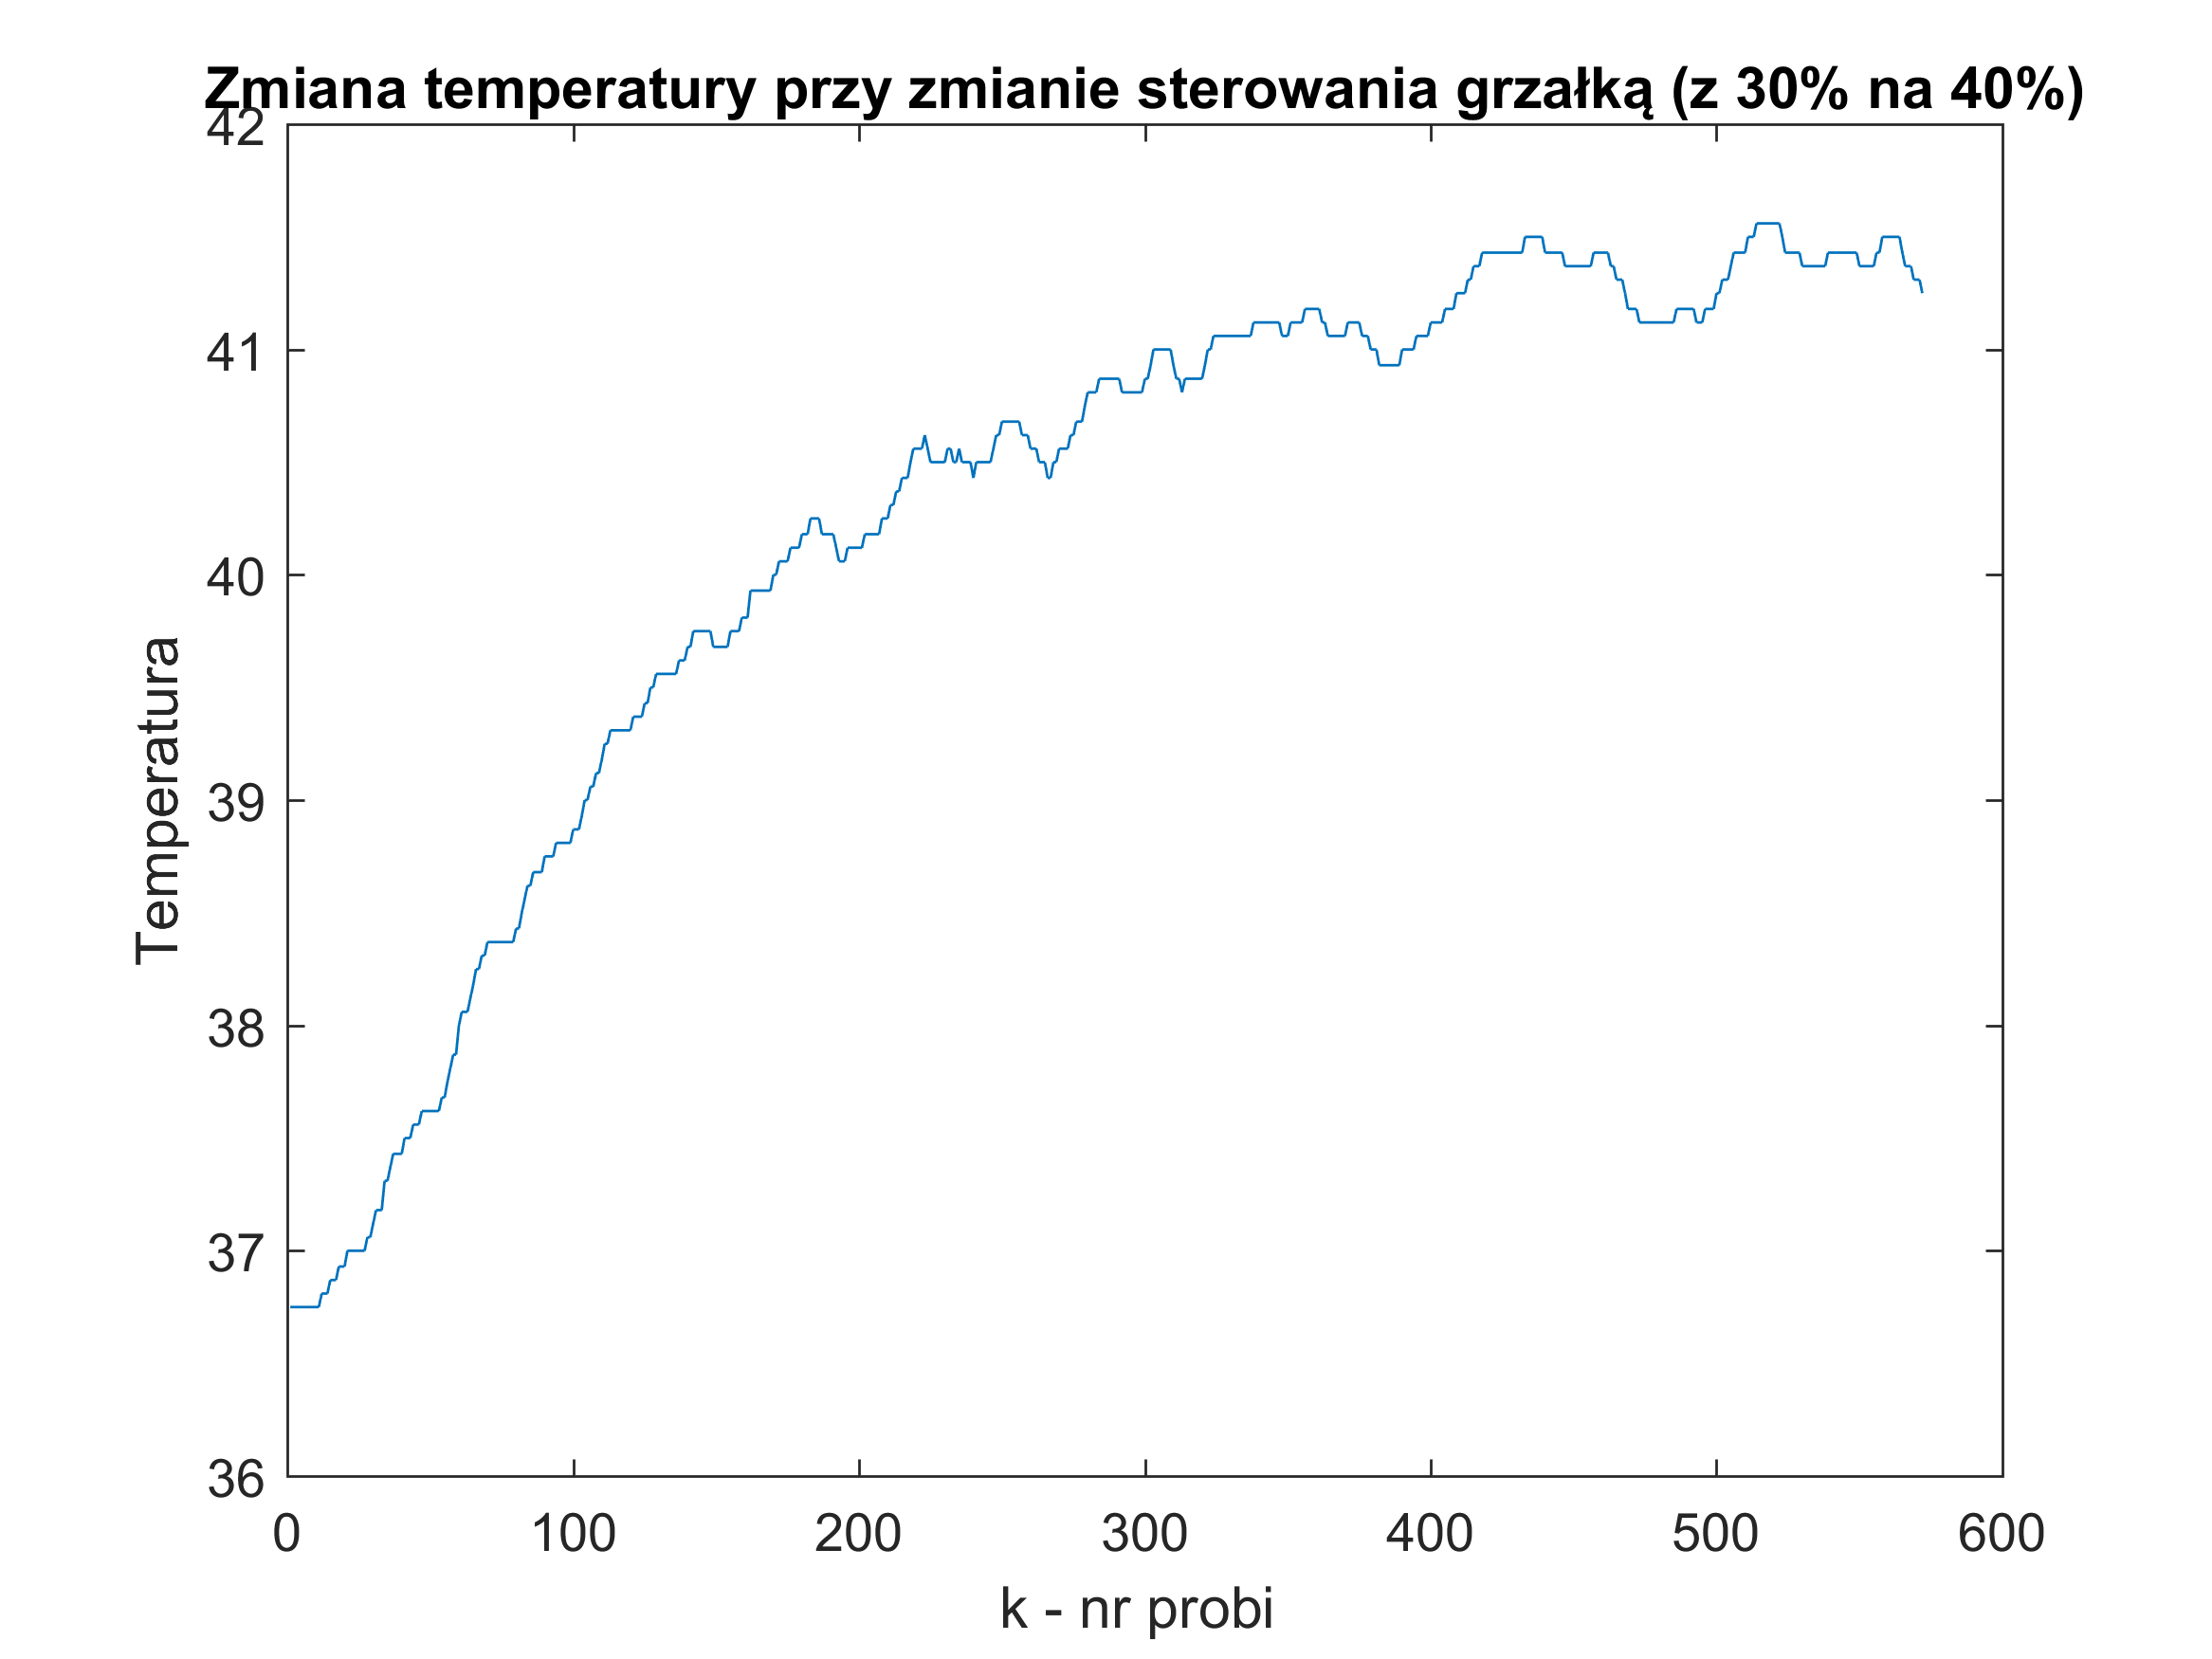
\includegraphics[width=0.9\linewidth]{nnor_od_skok_gg}
	\caption{Przebieg temperatury przy zmianie sterowania grzałką z $30\%$ na $40\%$}
	\label{fig:nnosgg}
\end{figure}
\begin{figure}[H]
	\centering
	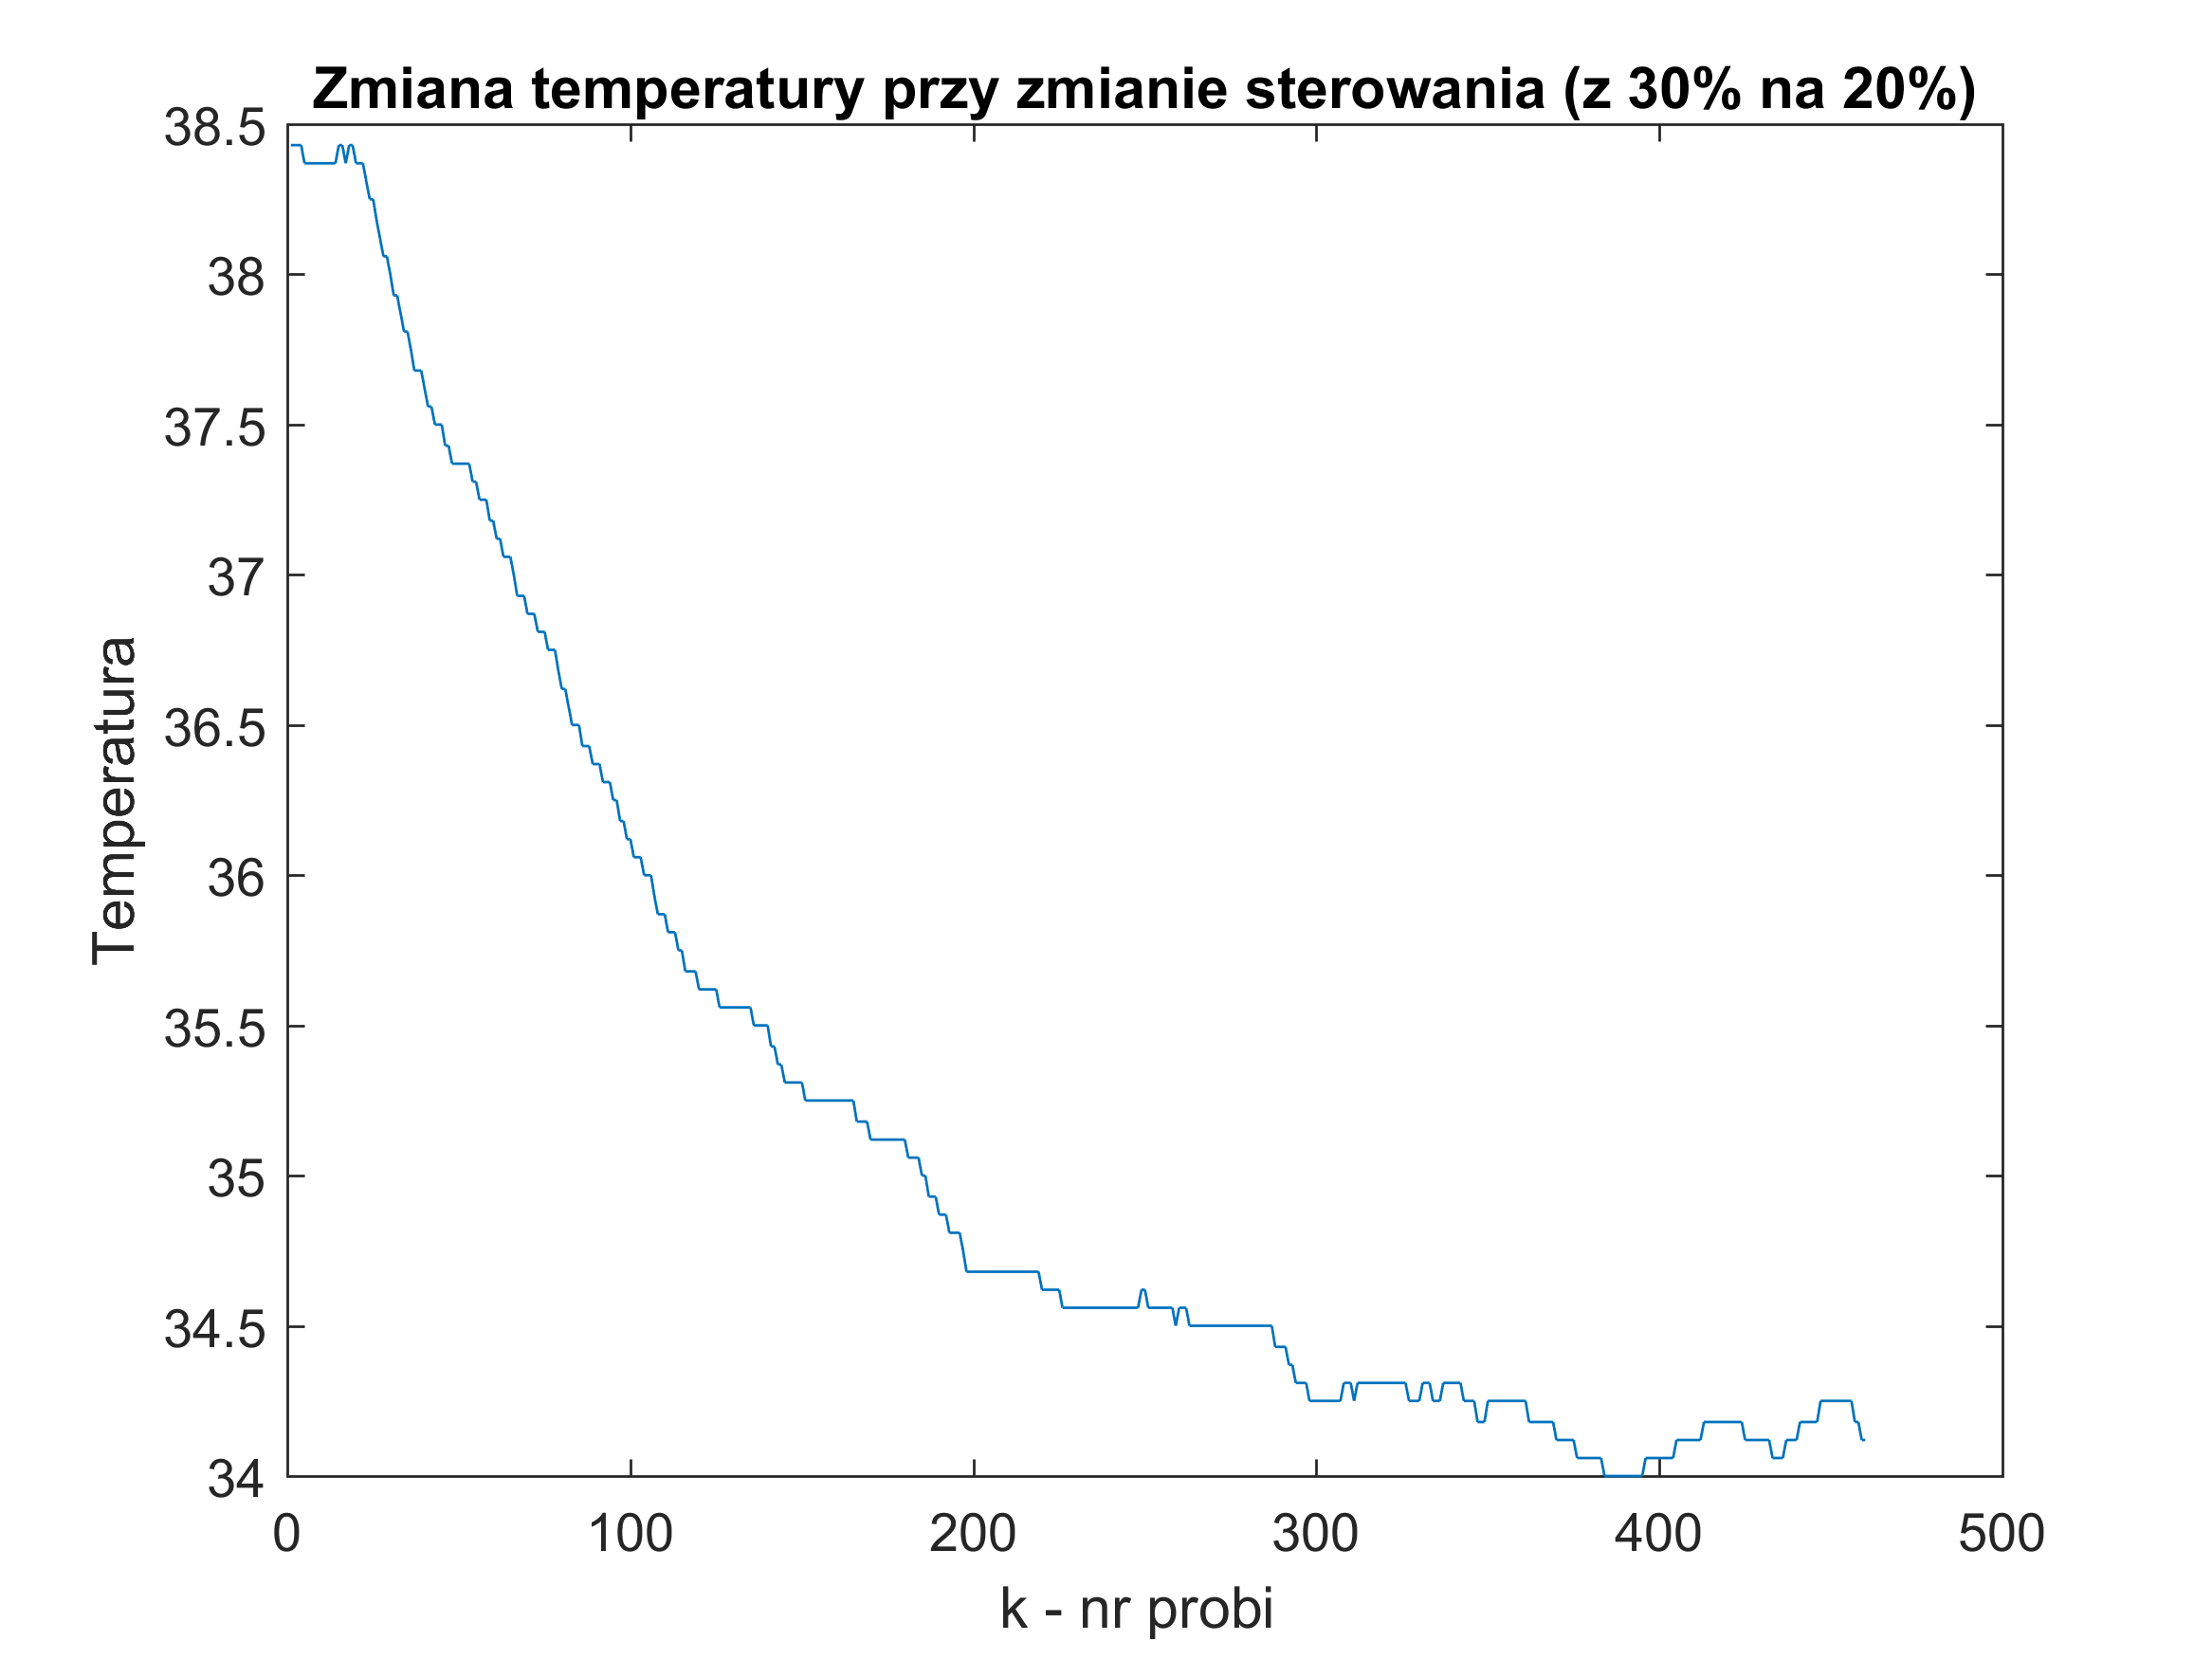
\includegraphics[width=0.9\linewidth]{nnor_od_skok_gd}
	\caption{Przebieg temperatury przy zmianie sterowania grzałką z $30\%$ na $20\%$}
	\label{fig:nnosgd}
\end{figure}
Aby poprawnie zanalizować uzyskane odpowiedzi skokowe należy je znormalizować: \\
1. od każdej wartości wyjścia obiektu - temperatur należy odjąć wartość wyjścia obiektu w chwili sprzed dokonania zmiany sterownia,\\
2. należy podzielić tak uzyskany wektor przez zmianę sygnału sterującego.\\
Po dokonaniu normalizacji uzyskaliśmy następujące przebiegi:
\begin{figure}[H]
	\centering
	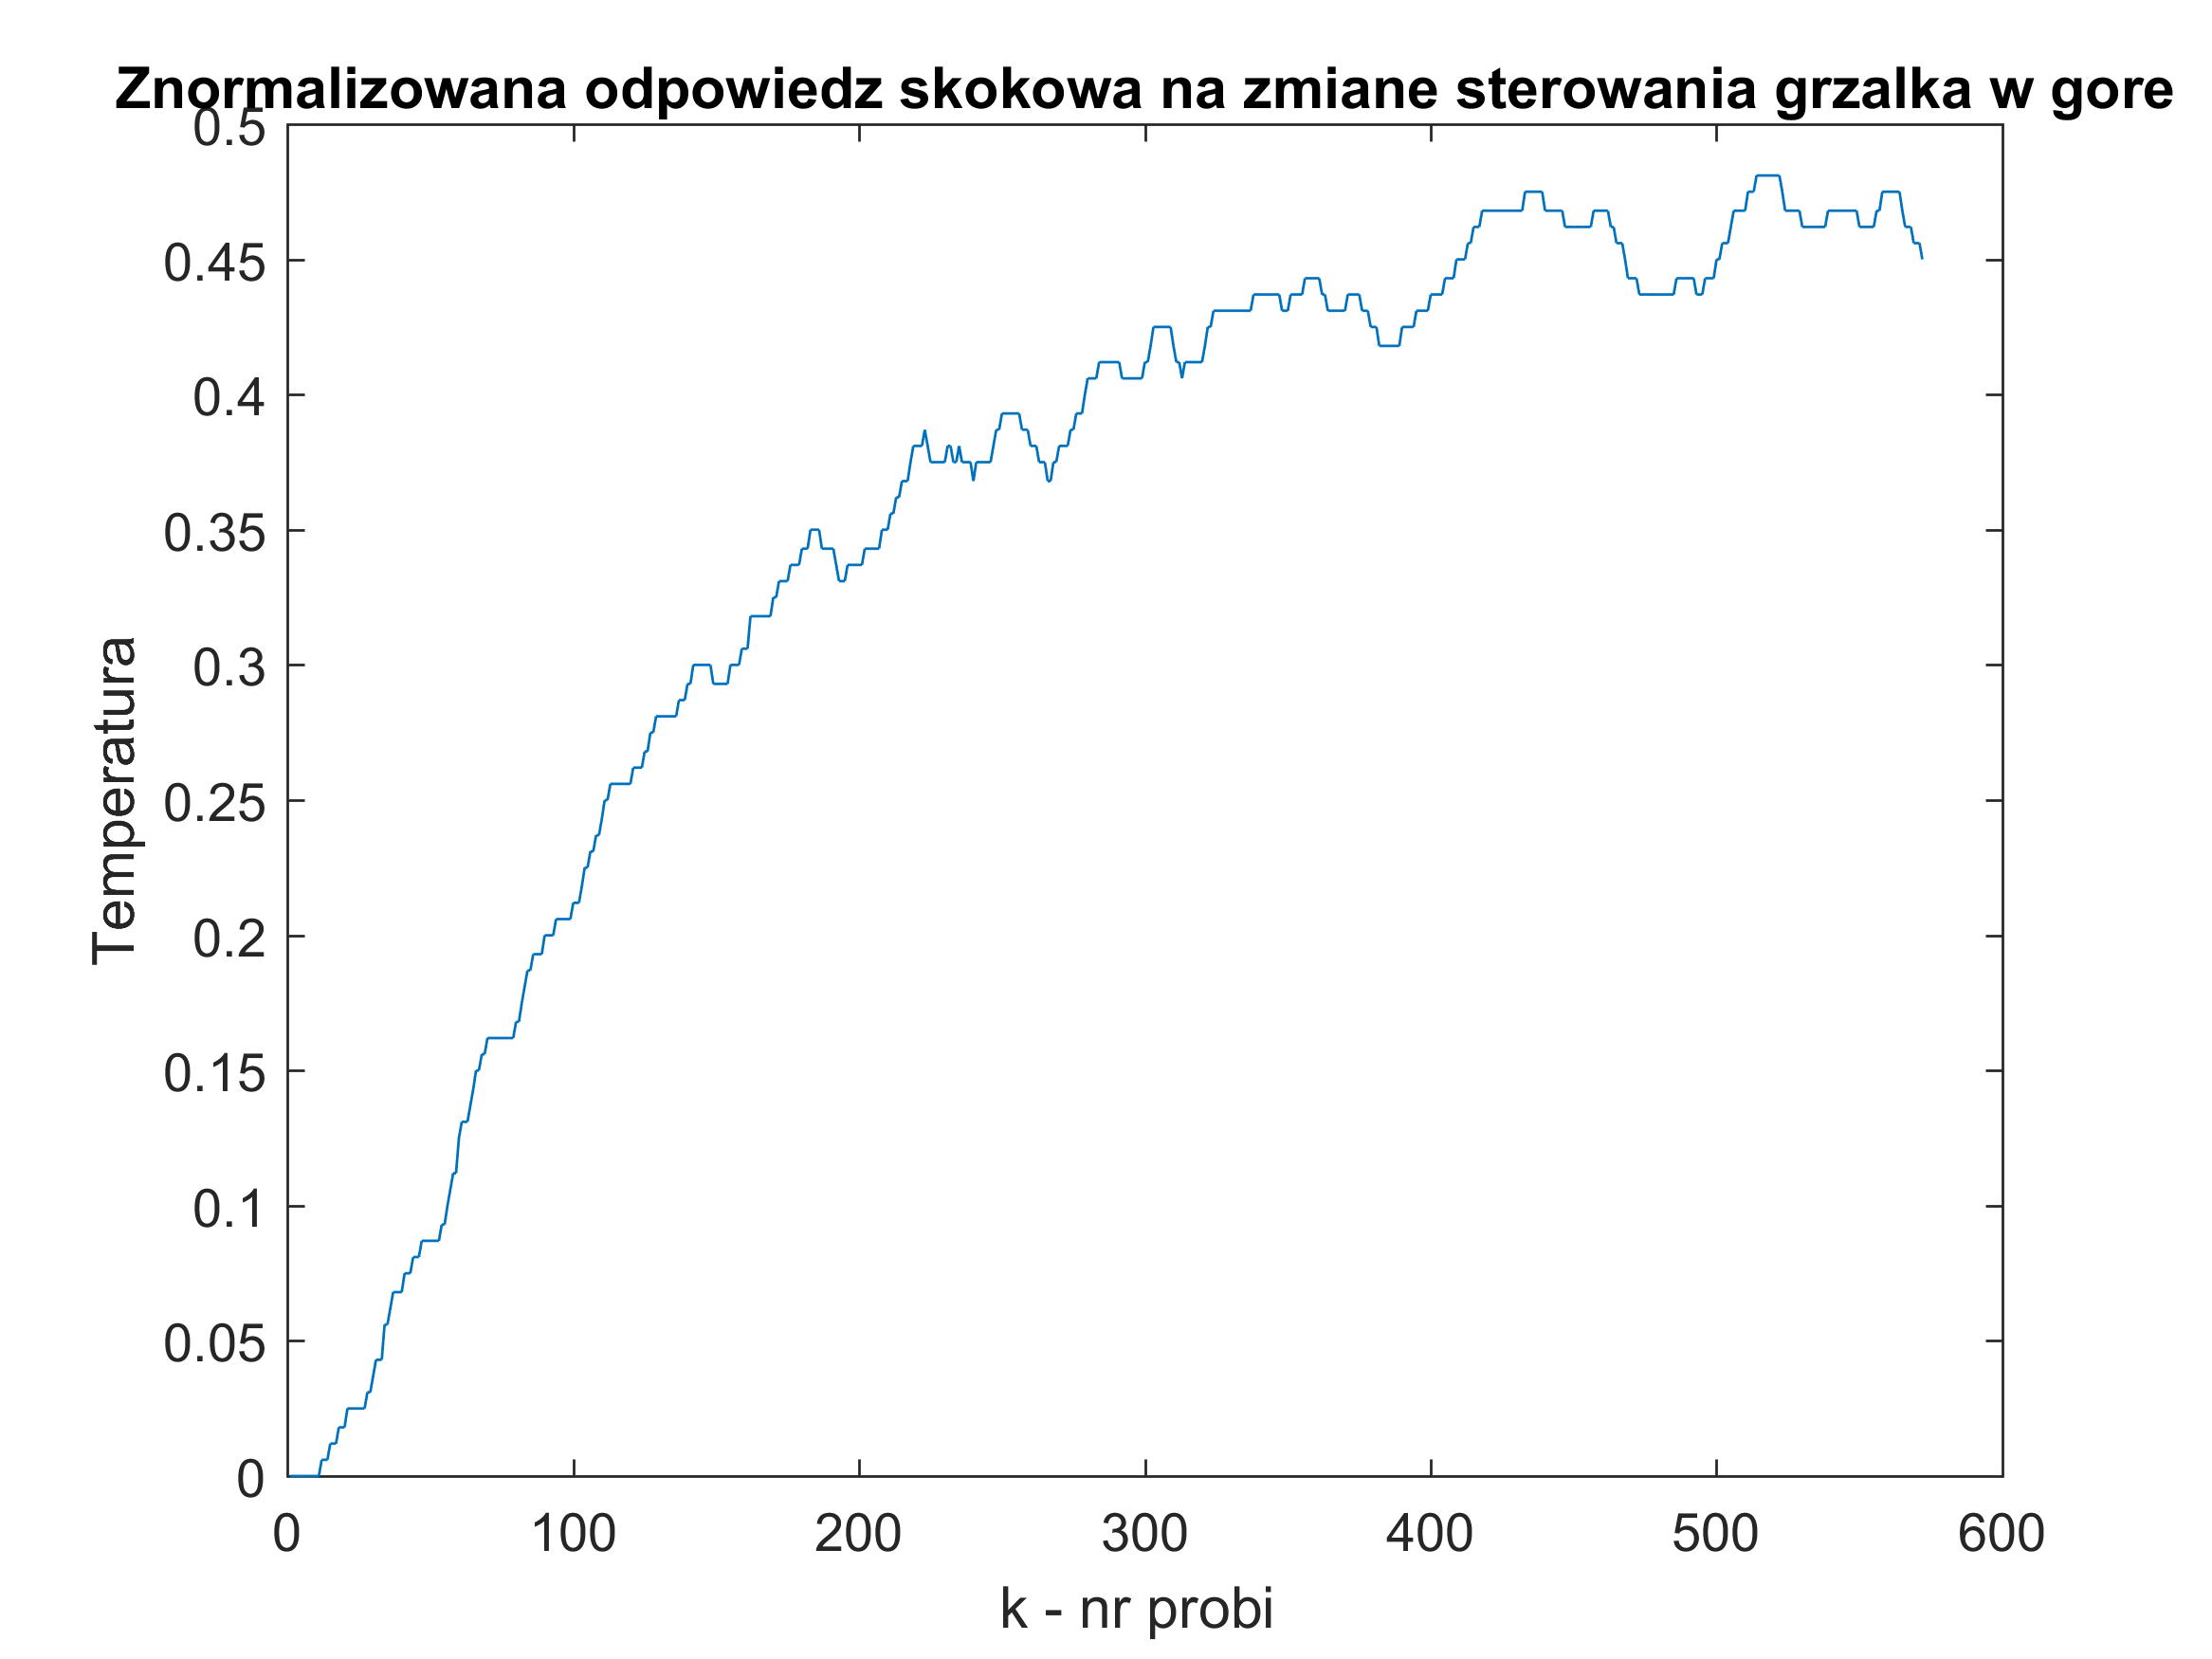
\includegraphics[width=0.9\linewidth]{nor_od_skok_gg}
	\caption{Znormalizowana odpowiedź skokowa na zmianę sterowania grzałką z $30\%$ na $40\%$}
	\label{fig:nosgg}
\end{figure}
\begin{figure}[H]
	\centering
	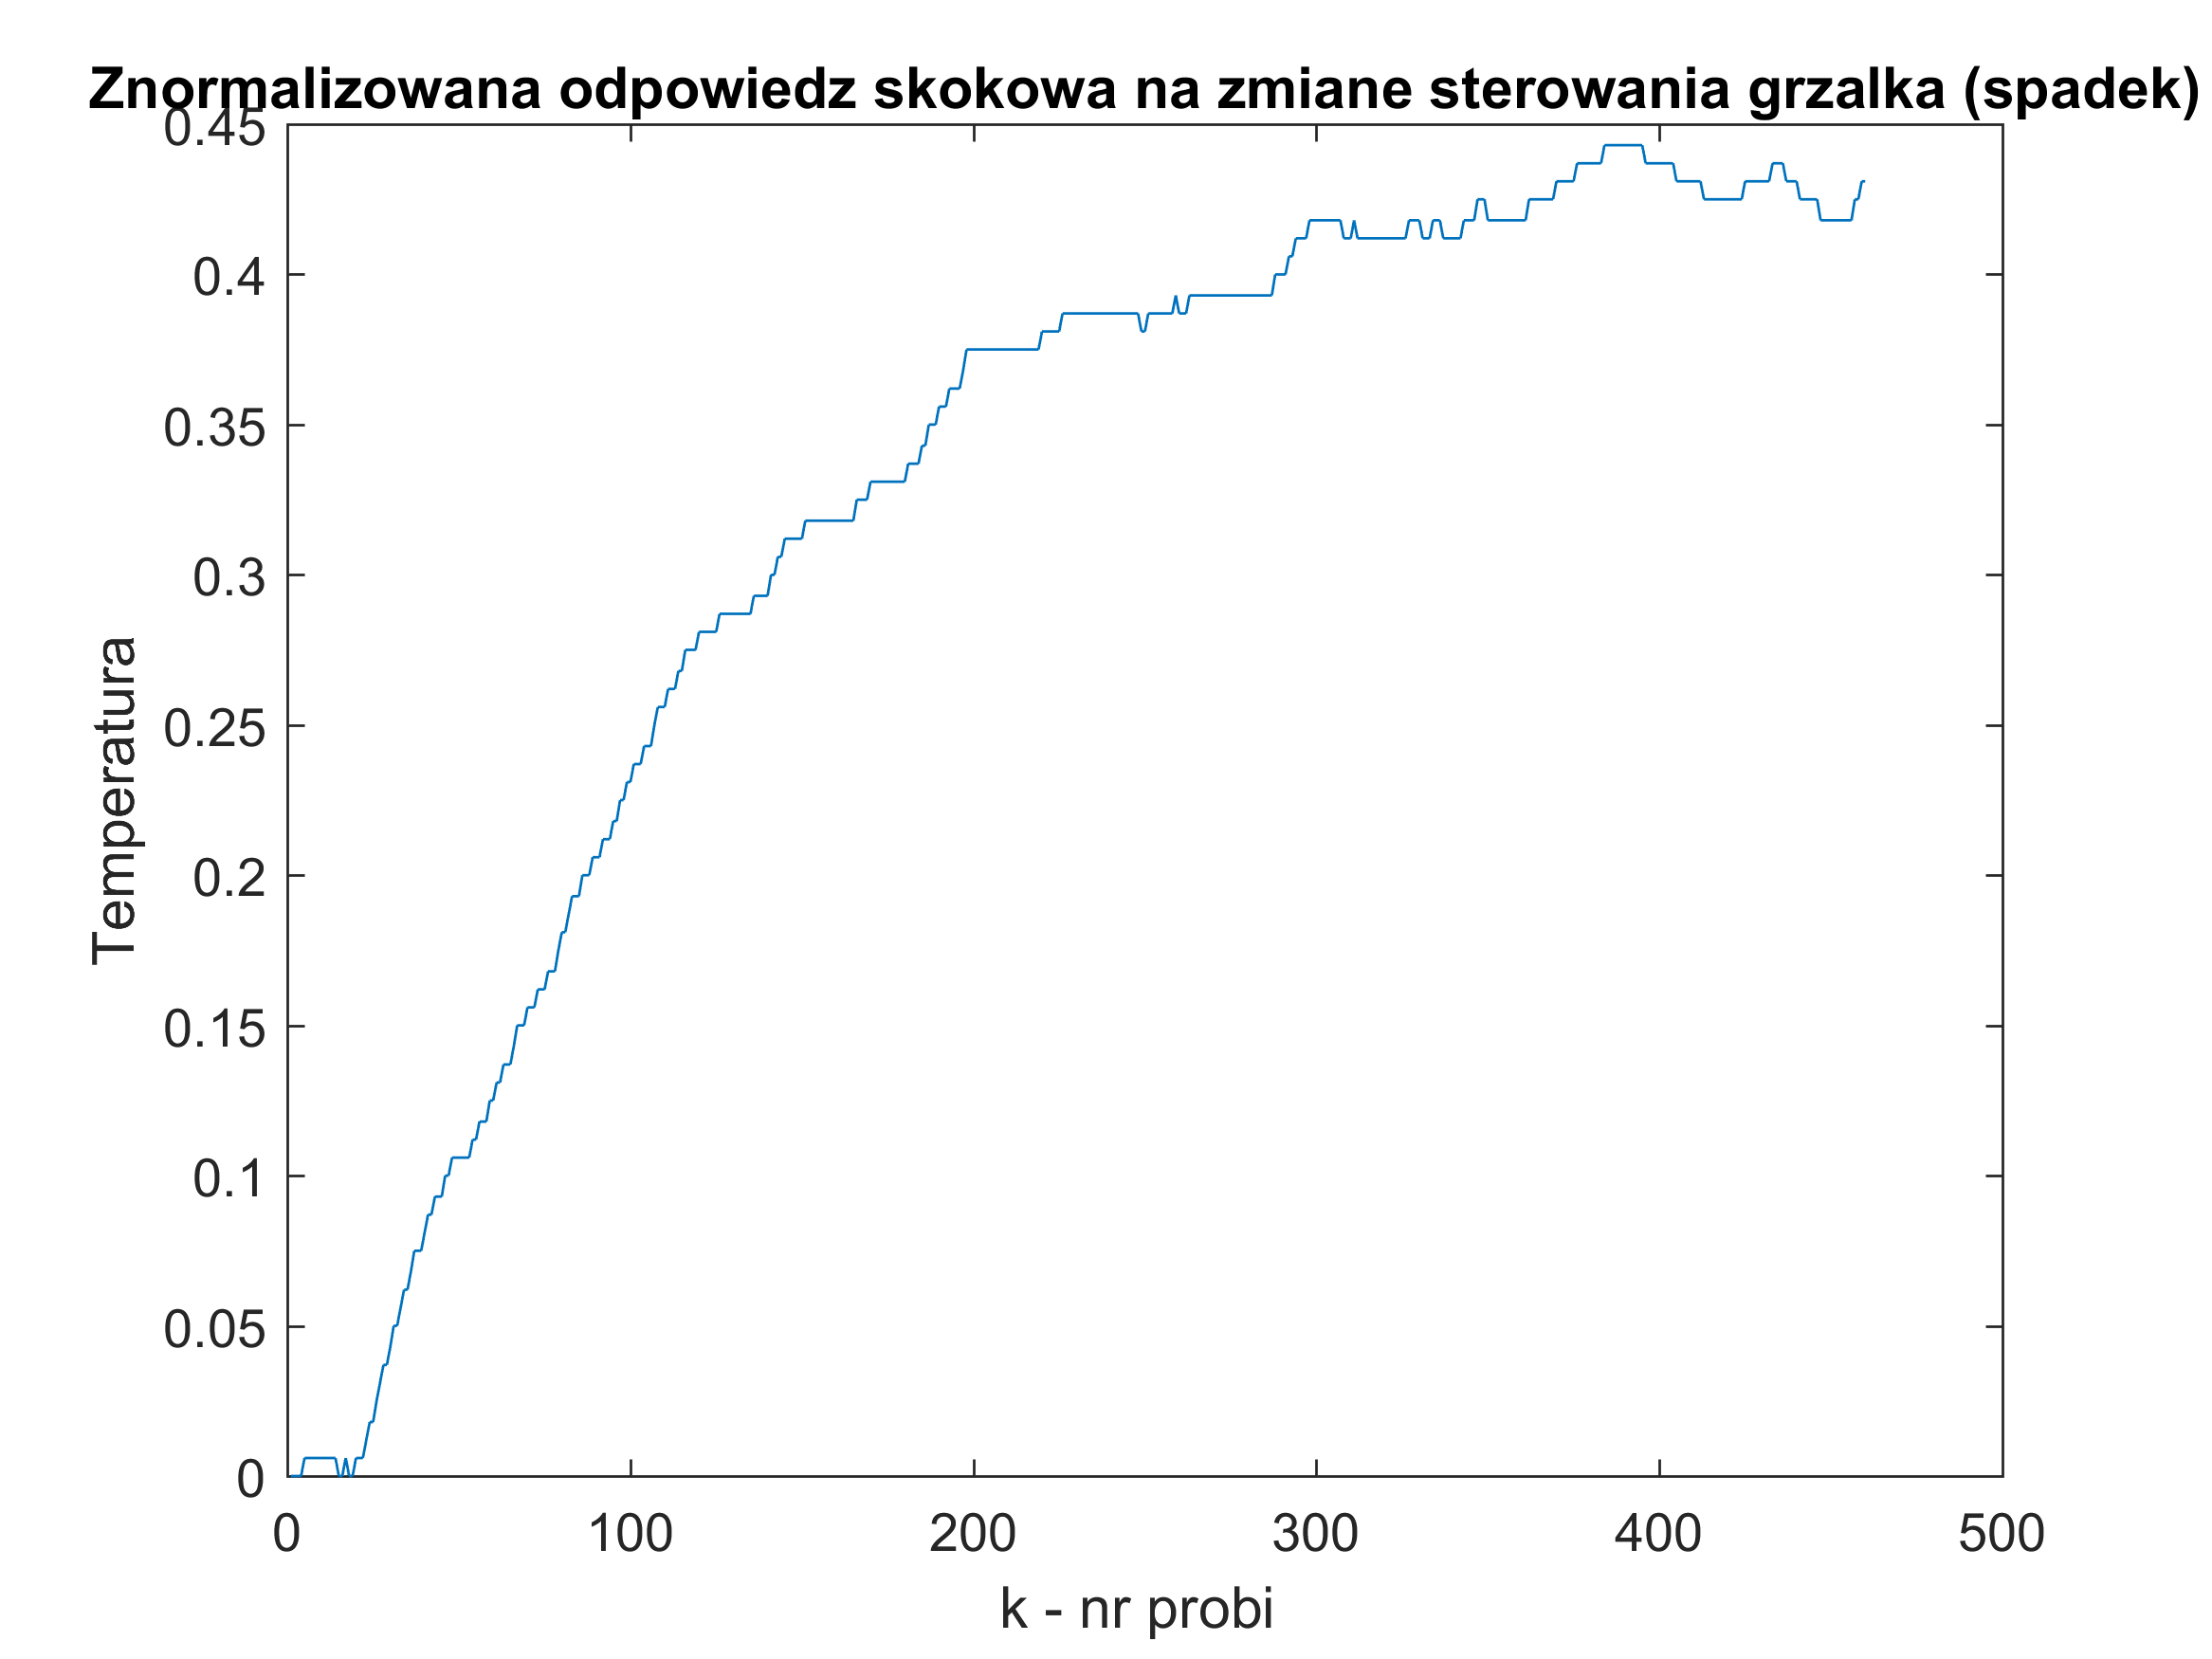
\includegraphics[width=0.9\linewidth]{nor_od_skok_gd}
	\caption{Znormalizowana odpowiedź skokowa na zmianę sterowania grzałką z $30\%$ na $20\%$}
	\label{fig:nosgd}
\end{figure}
Zauważyliśmy, że przebieg obu odpowiedzi skokowych przypomina swoją trajektorią przebieg odpowiedzi skokowej obiektu z pojedynczą inercją i odpóźnieniem. Obiekt taki można opisać następującą transmitancją:
\[G(s)=e^{-\tau \cdot s} \cdot \frac{K}{T_{0} \cdot s +1}\]
W celu ustalenia parametrów modelu (parametry $\tau$, $K$ i $T_{0}$) wykorzystaliśmy metodę graficzną. Metoda ta pozwala na odczytanie owych parametrów z wykresu. Z racji tego, że nasz regulator wysyłał sterownia co 1s, numer próbki odpowiada kolejnym sekundom eksperymentu. \\
Przyjmuje się, że $\tau$ równe jest czasowi, po którym sygnał wyjściowy (temperatura), zaczyna reagować na zmianę sterowania.\\
Parametr $K$ przyjmuje się jako wartość, na jakiej stabilizuje się znormalizowana odpowiedź skokowa.\\
Stałą $T_{0}$ ustala się jako czas, po którym wartość wyjścia osiągnie $63\%$ wartości wzmocnienia obiektu od momentu zauważenia zmiany sygnału wyjściowego (opóźnienie się nie wlicza.)\\ 
Dla zmiany sygnału sterującego grzałką z $30\%$ na $40\%$ odczytane zostały następujące wartości parametrów modelu:
\[\tau=11\]
\[K=0,46\]
\[T_{0}=127\]
Na wykresie \ref{fig:transmi_gglep} można zauważyć, że wyjście obiektu z tak obliczoną transmitancją w zadawalającym stopniu pokrywa się z uzyskaną odpowiedzią skokową. Aby delikatnie poprawić jakość modelu parametry zmodyfikowane zostały do następujących wartości:
\[\tau=15\]
\[K=0,47\]
\[T_{0}=130\]
Na podstawie wykresów \ref{fig:nosgg} i \ref{fig:nnosgd} można zauważyć, że obiekt delikatnie inaczej zachowuje się dla wzrostu i spadku wartości sygnału sterującego. Z tego powodu, transmitancja, jaka została wykorzystana w późniejszych krokach odbiega od obliczonej transmitancji. Parametry ostatecznie przyjętej transmitancji:
\[\tau=19\]
\[K=0,46\]
\[T_{0}=120\]
\begin{figure}[H]
	\centering
	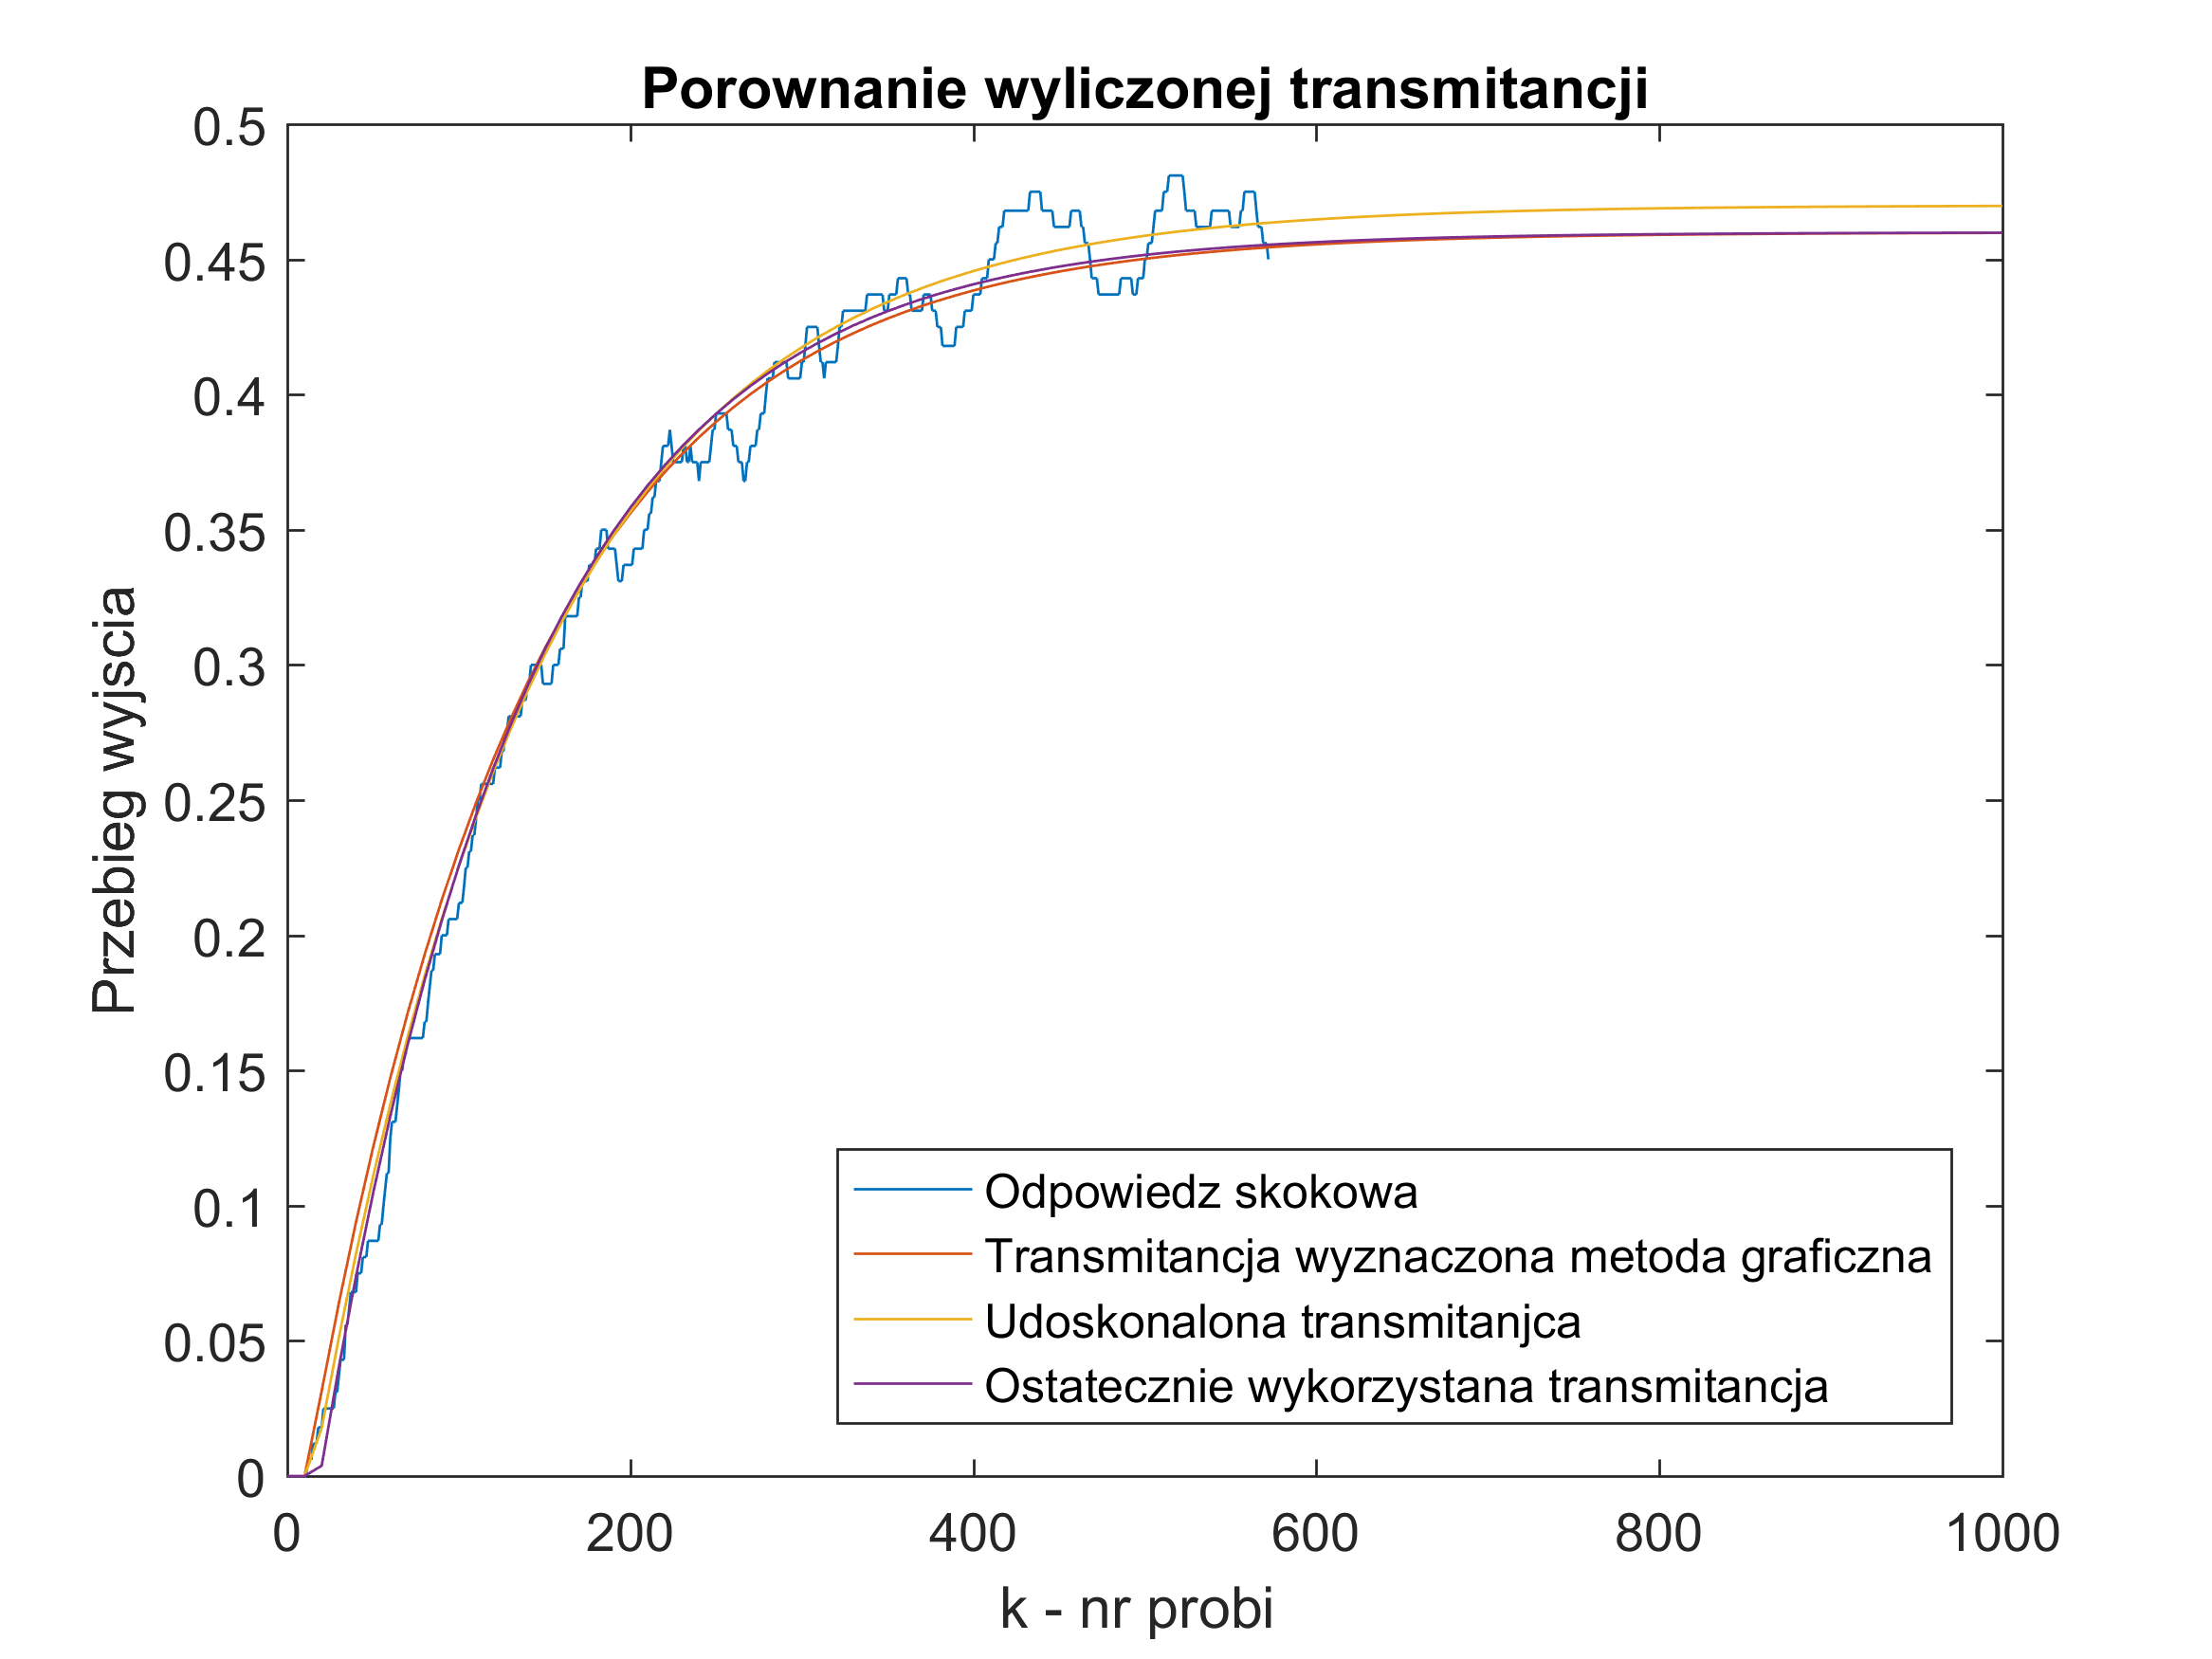
\includegraphics[width=0.9\linewidth]{transmi_gglep}
	\caption{Porównanie przebiegów odpowiedzi skokowej i obliczonych transmitancji}
	\label{fig:transmi_gglep}
\end{figure}
Dla zmiany sygnału sterującego grzałką z $30\%$ na $20\%$ odczytane zostały następujące wartości parametrów modelu:
\[\tau=19\]
\[K=0,431\]
\[T_{0}=115\]
Zgodnie z przewidywaniami odbiegają one od wartości obliczonych dla wzrostu sygnału sterującego grzałką. Z wykresu \ref{fig:transmi_gd} wynika, że transmitancja wyznaczona metodą graficzną nienajlepiej modeluje zadany obiekt. W celu udoskonalenia modelu obiektu na spadek sterowania grzałką parametry zostały zmodyfikowane do:
\[\tau=19\]
\[K=0,431\]
\[T_{0}=100\]
Na wykresie \ref{fig:transmi_gd} zaznaczony jest także przebieg transmitancji ostatecznie wybranej. Stanowi ona w pewien sposób połączenie obu modeli (odpowiedzi skokowe zarówno na wzrost i spadk sygnału sterującego grzałką). Taka postać transmitancji została wykorzystana w bloku odprzęgającym zakłócenia oraz w programie do strojenia regulatora PID.
\begin{figure}[H]
	\centering
	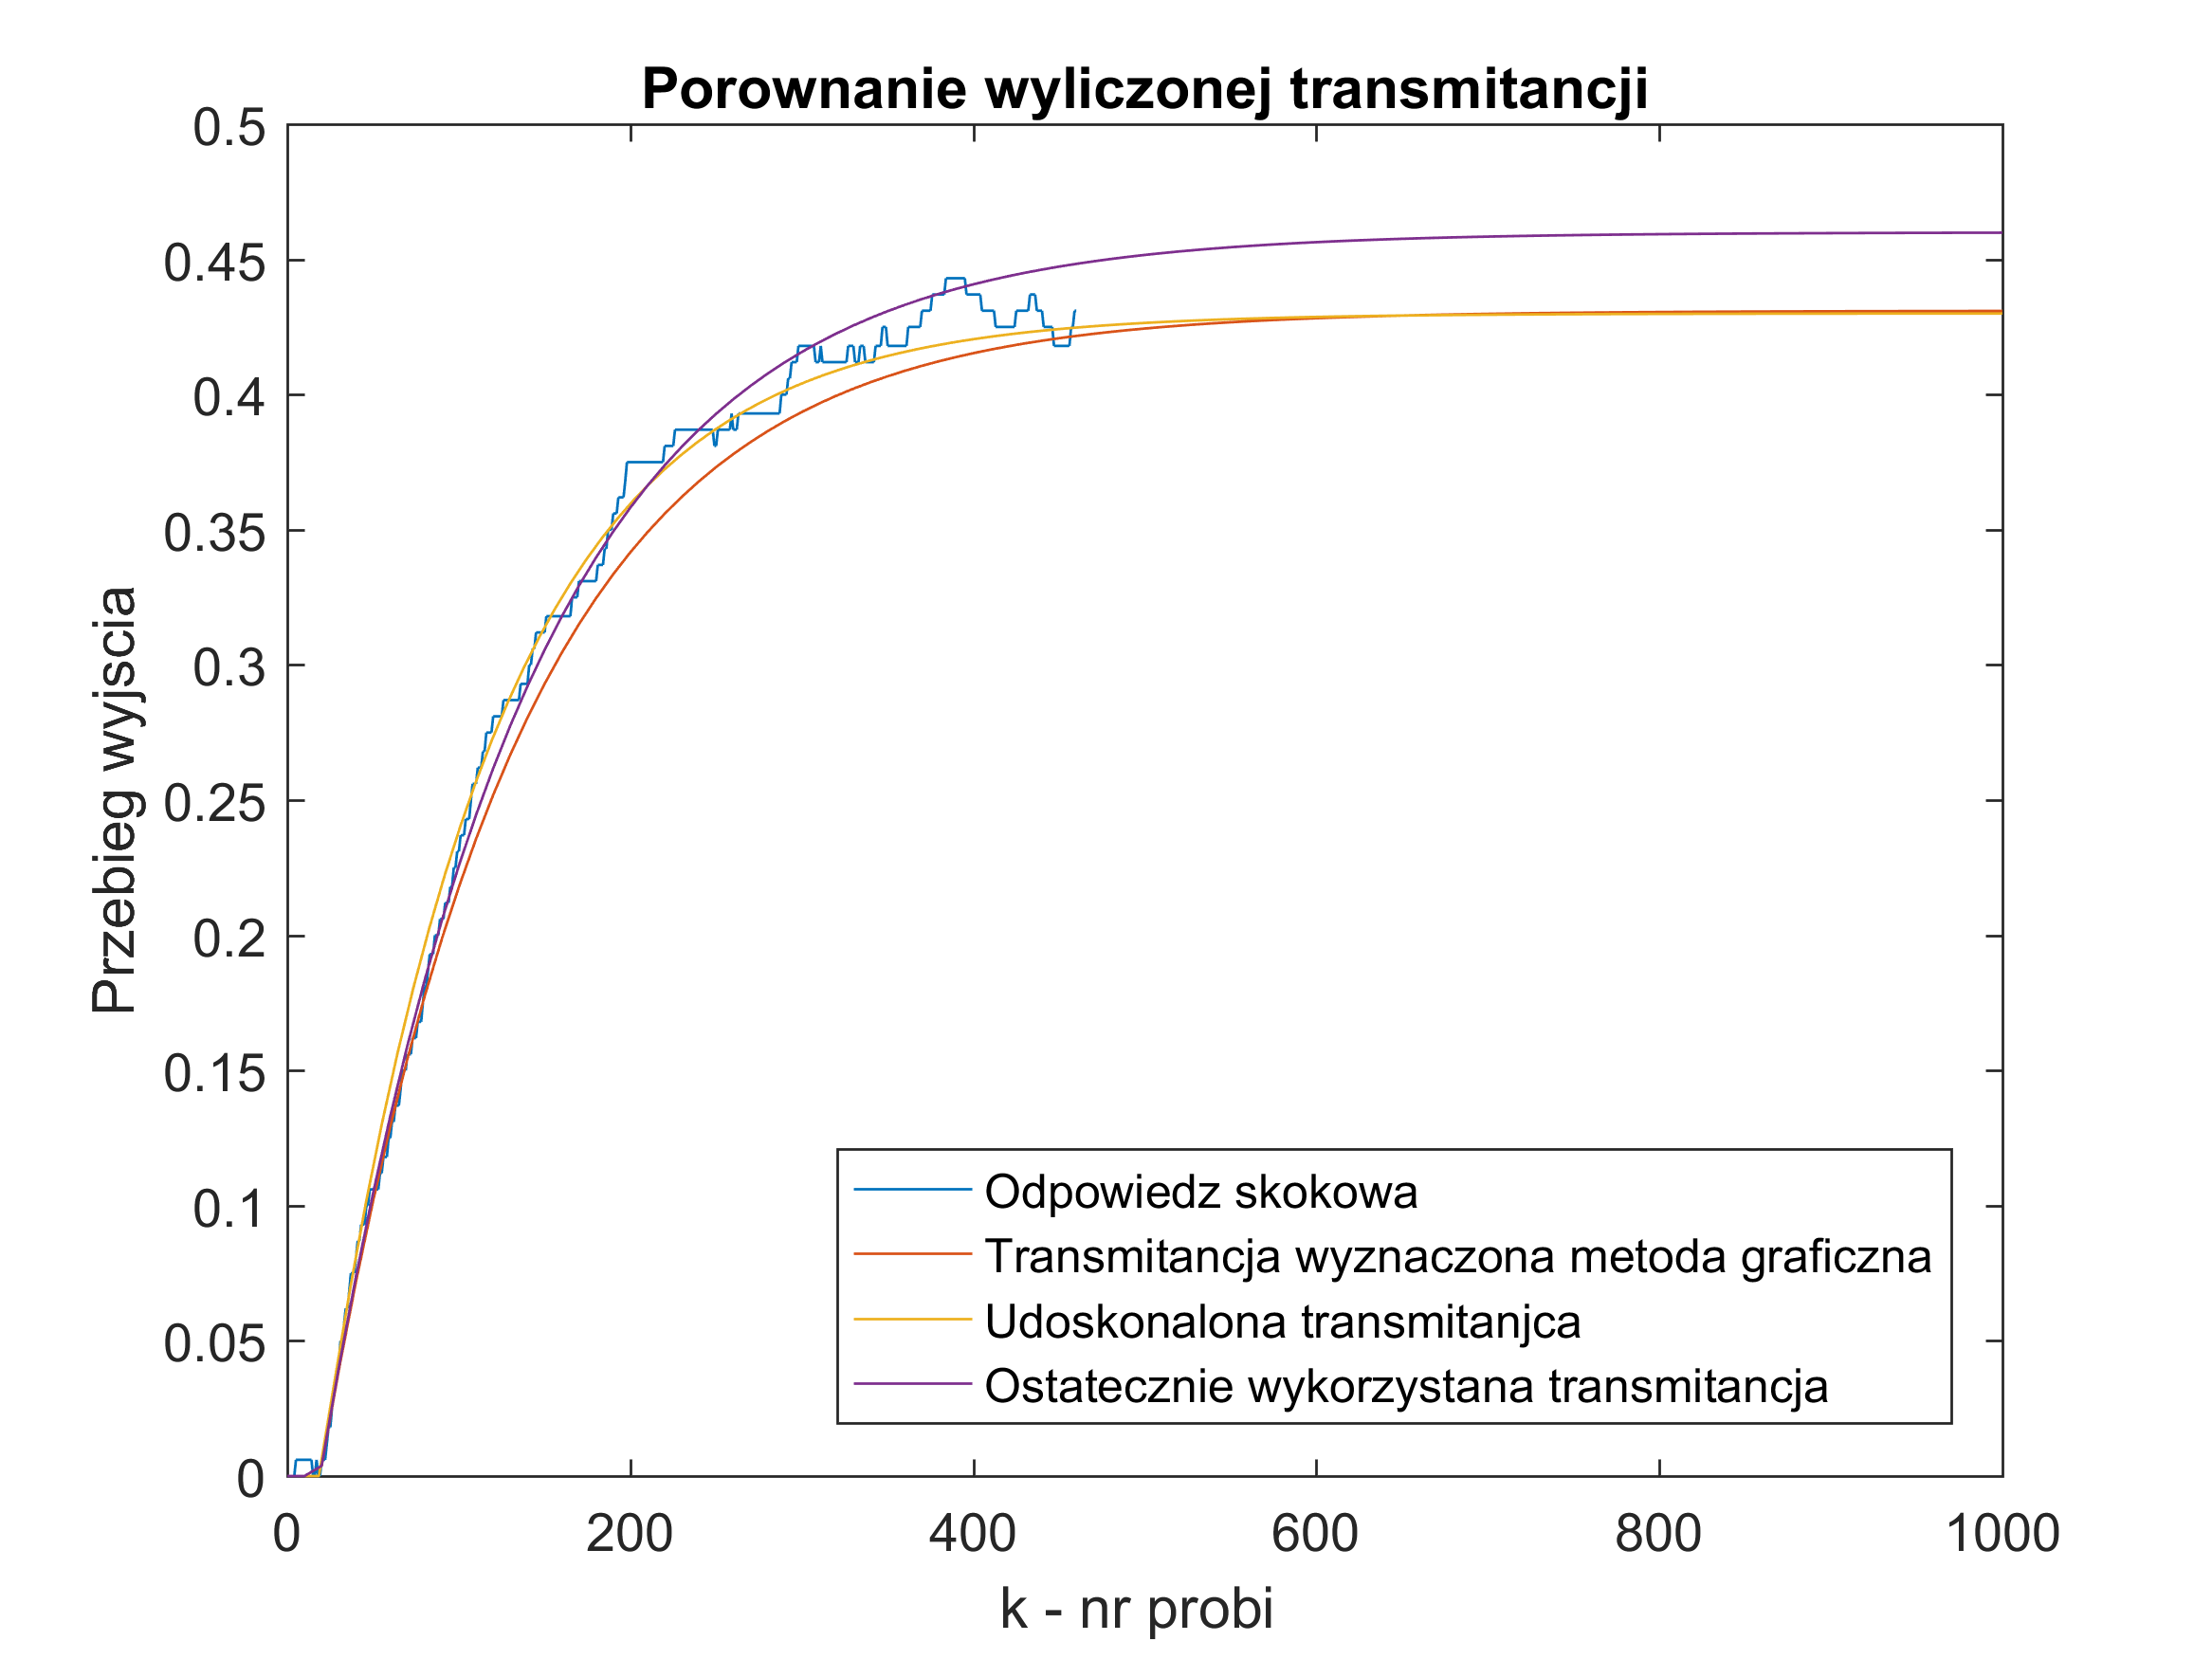
\includegraphics[width=0.9\linewidth]{transmi_gd}
	\caption{Porównanie przebiegów odpowiedzi skokowej i obliczonych transmitancji}
	\label{fig:transmi_gd}
\end{figure}
Ostatecznie została przyjęta następująca postać transmitancji obiektu:
\[T_{0}(s)=e^{-19 \cdot s} \cdot \frac{0,46}{120 \cdot s +1}\]

\subsection{Identyfikacja obiektu - wentylator}
Takie same eksperymenty wykonaliśmy dla zmiany sygnału zakłócającego - wentylatora. Otrzymaliśmy następujące przebiegi:\\
\begin{figure}[H]
	\centering
	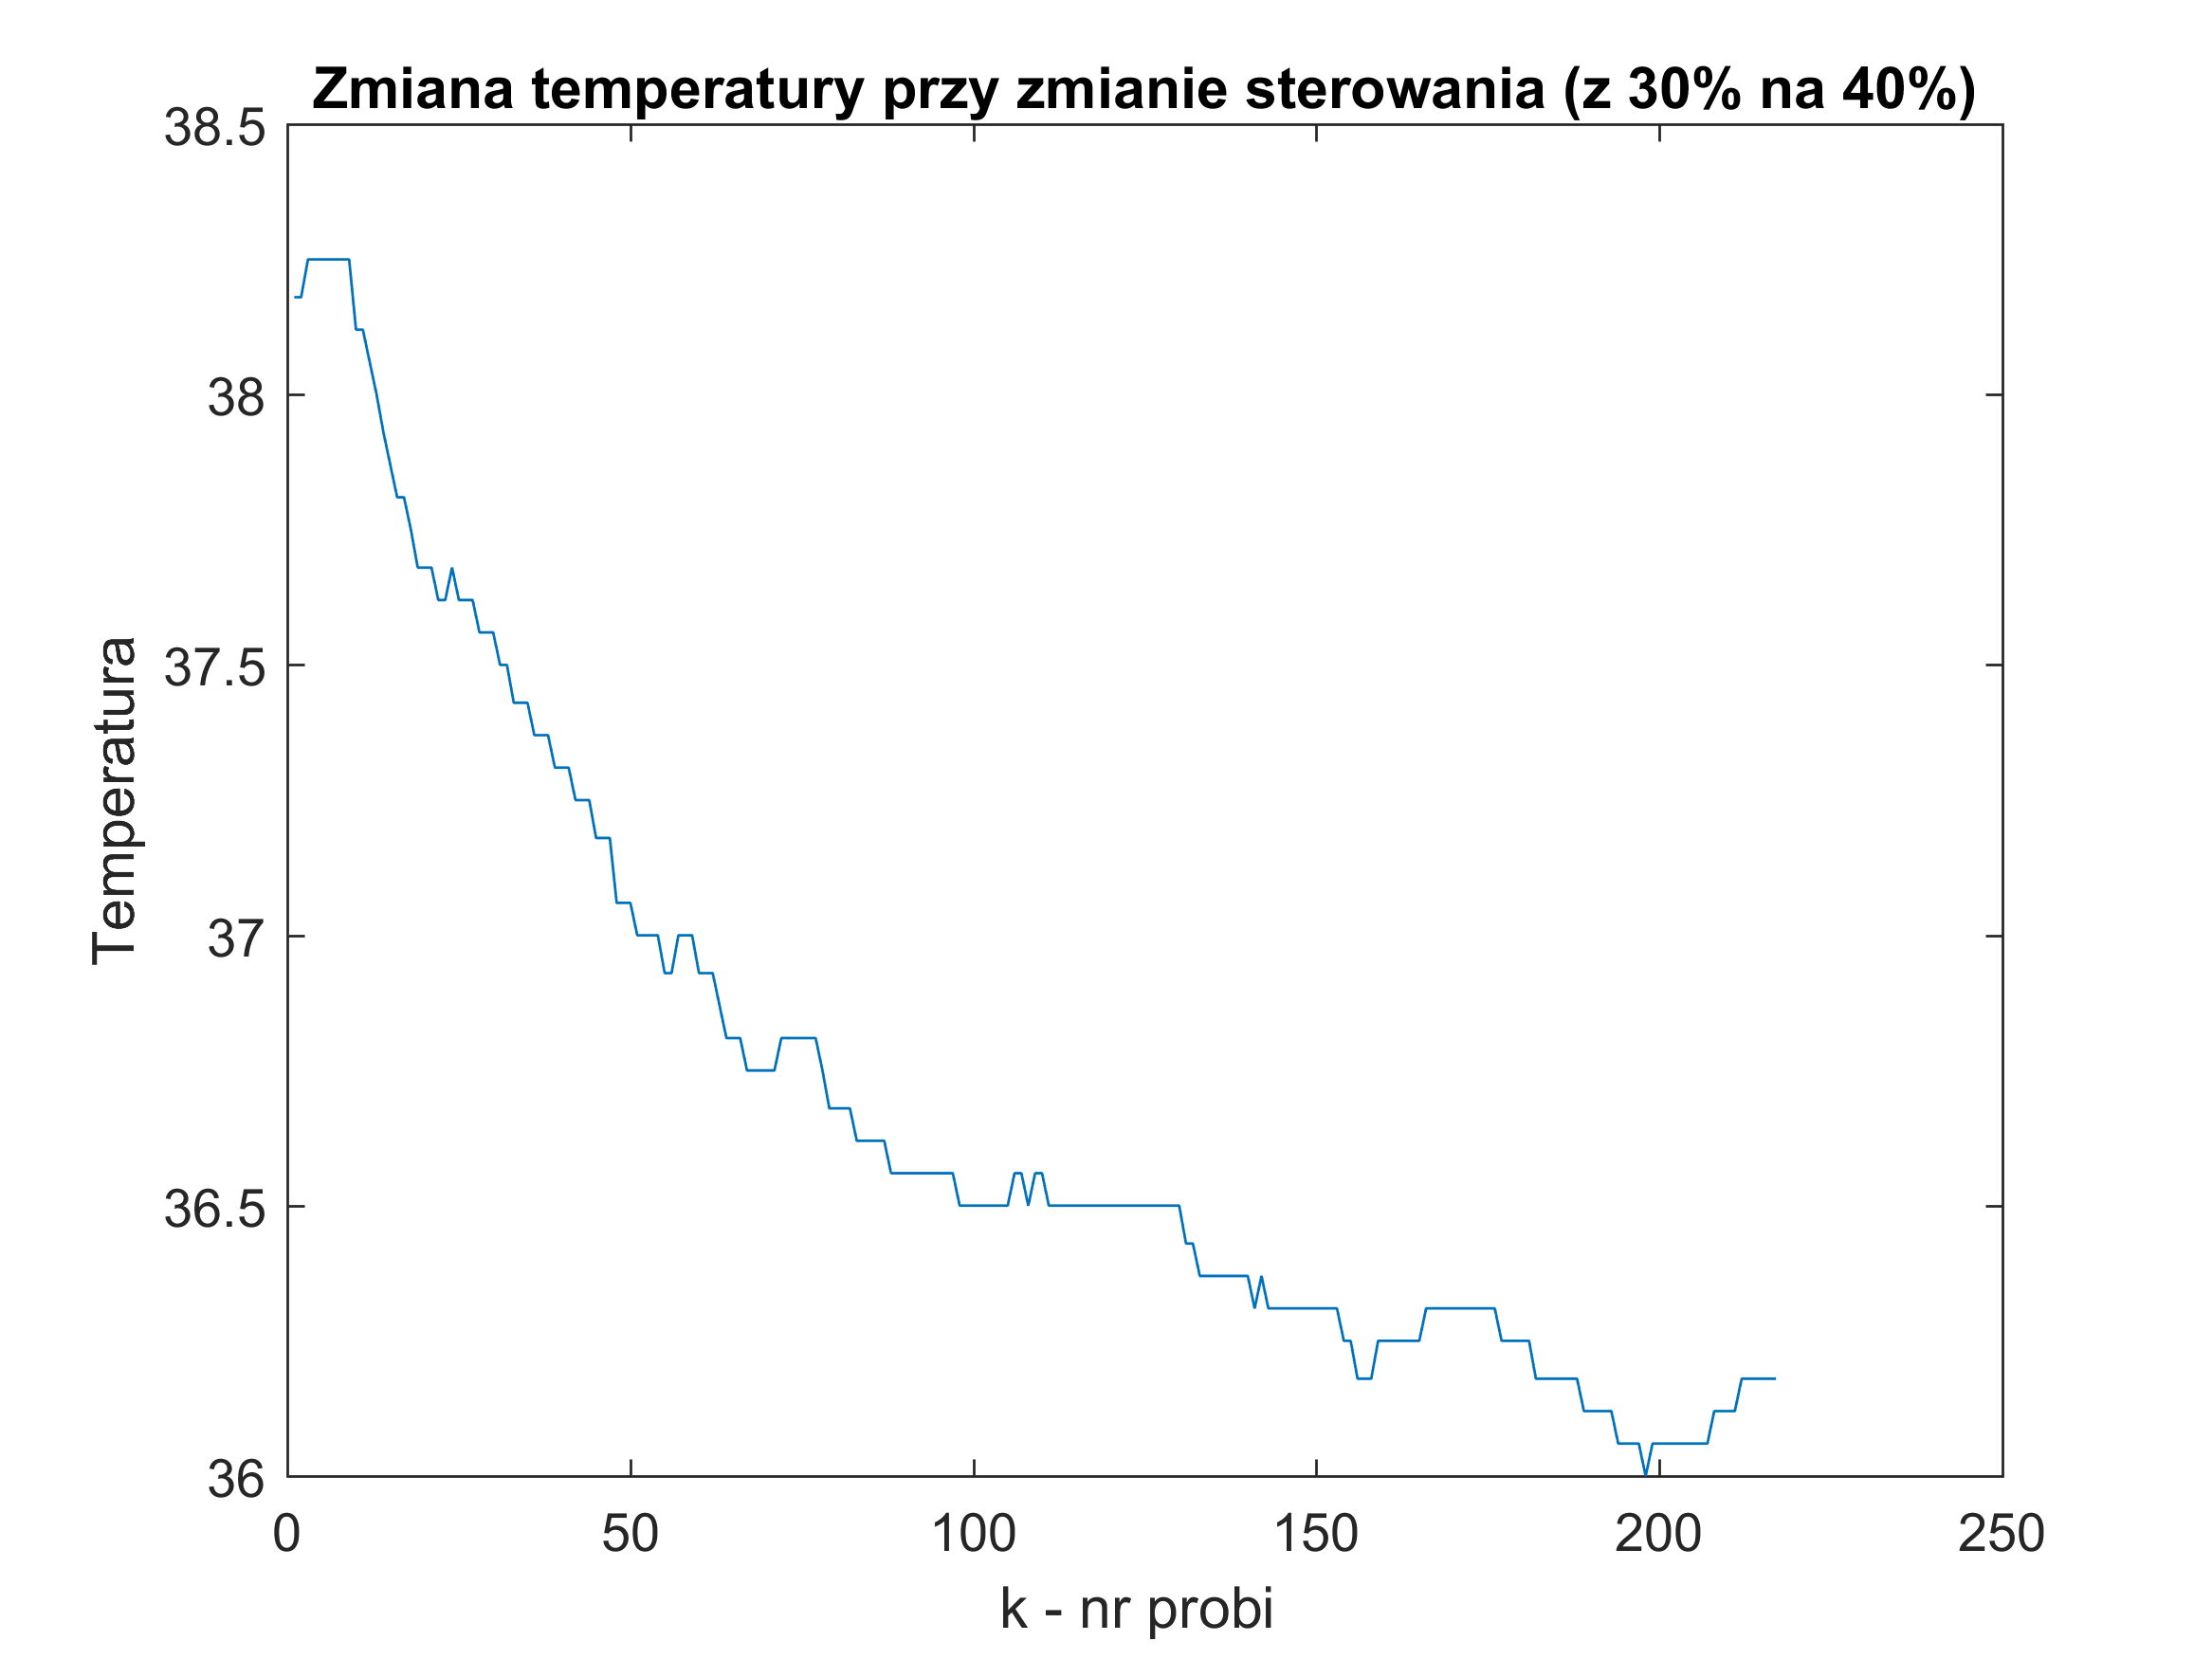
\includegraphics[width=0.9\linewidth]{nnor_od_skok_wg}
	\caption{Przebieg temperatury przy zmianie sterowania wentylatorem z $30\%$ na $40\%$}
	\label{fig:nnoswg}
\end{figure}
\begin{figure}[H]
	\centering
	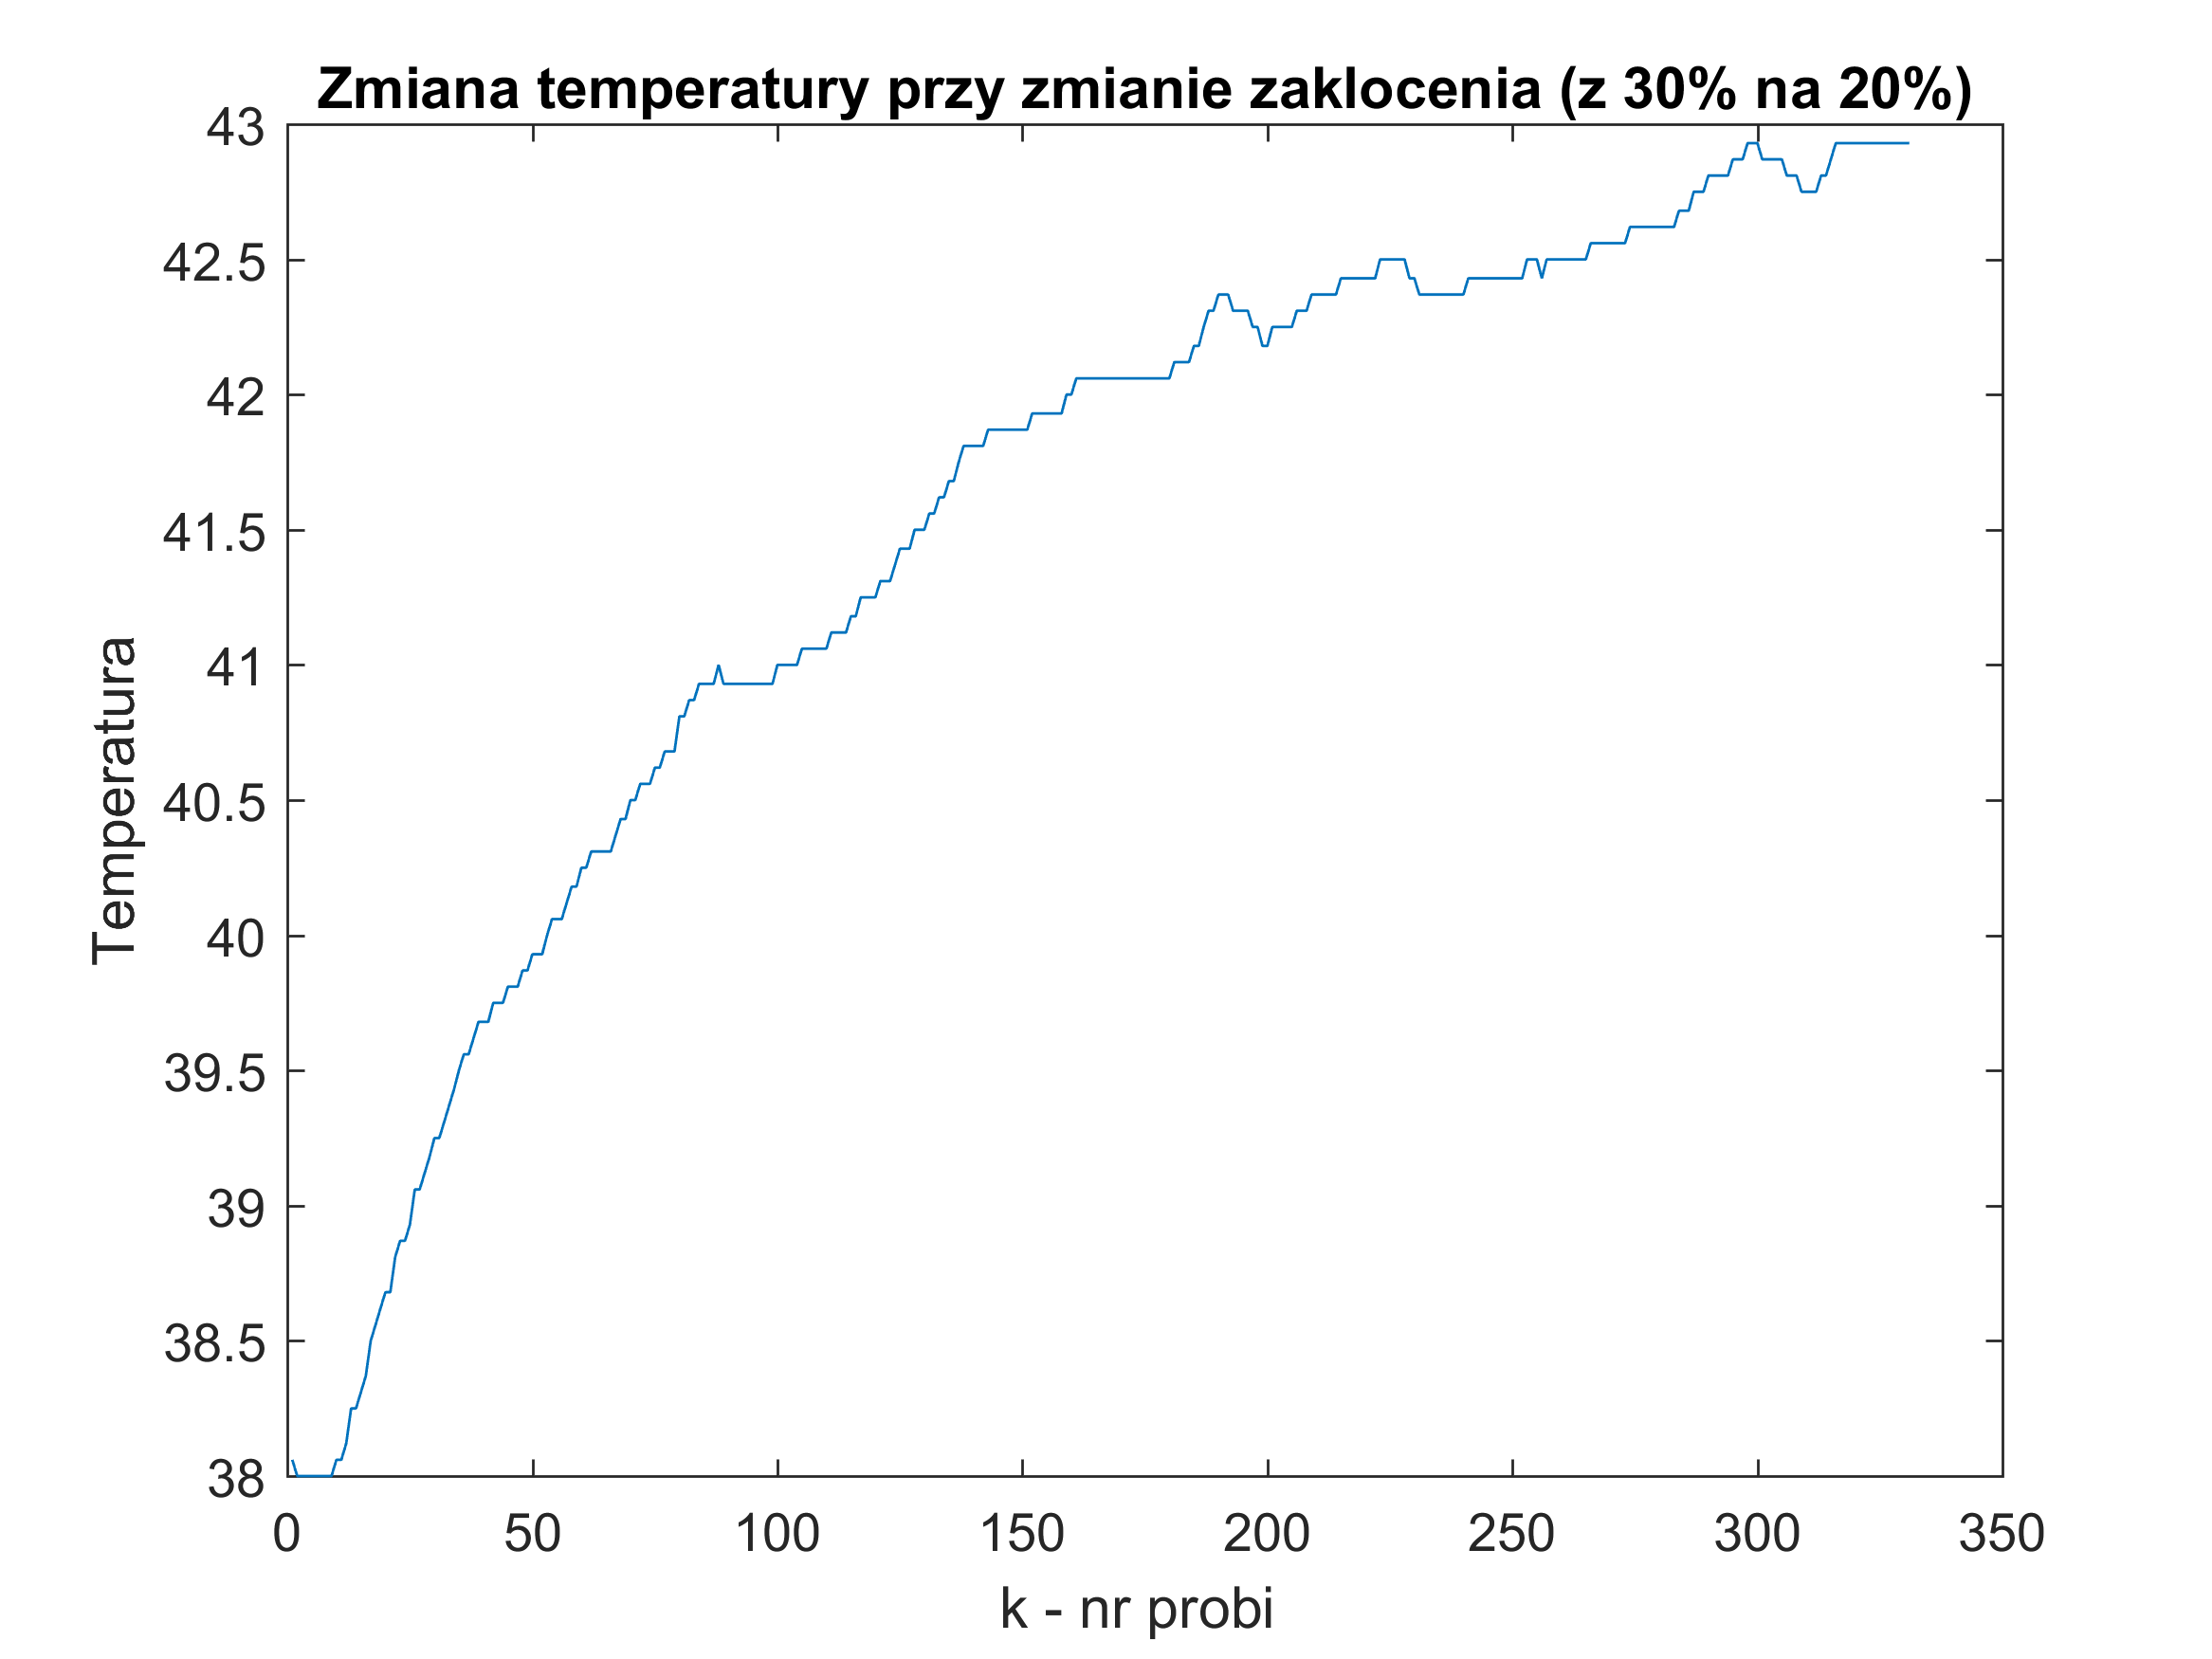
\includegraphics[width=0.9\linewidth]{nnor_od_skok_wd}
	\caption{Przebieg temperatury przy zmianie sterowania wentylatorem z $30\%$ na $40\%$}
	\label{fig:nnoswd}
\end{figure}
Przebiegi te zostały znormalizowane w taki sam sposób, jak zostało to opisane w punkcie \ref{grzalka}. Znormalizowane przebiegi mają następującą postać:
\begin{figure}[H]
	\centering
	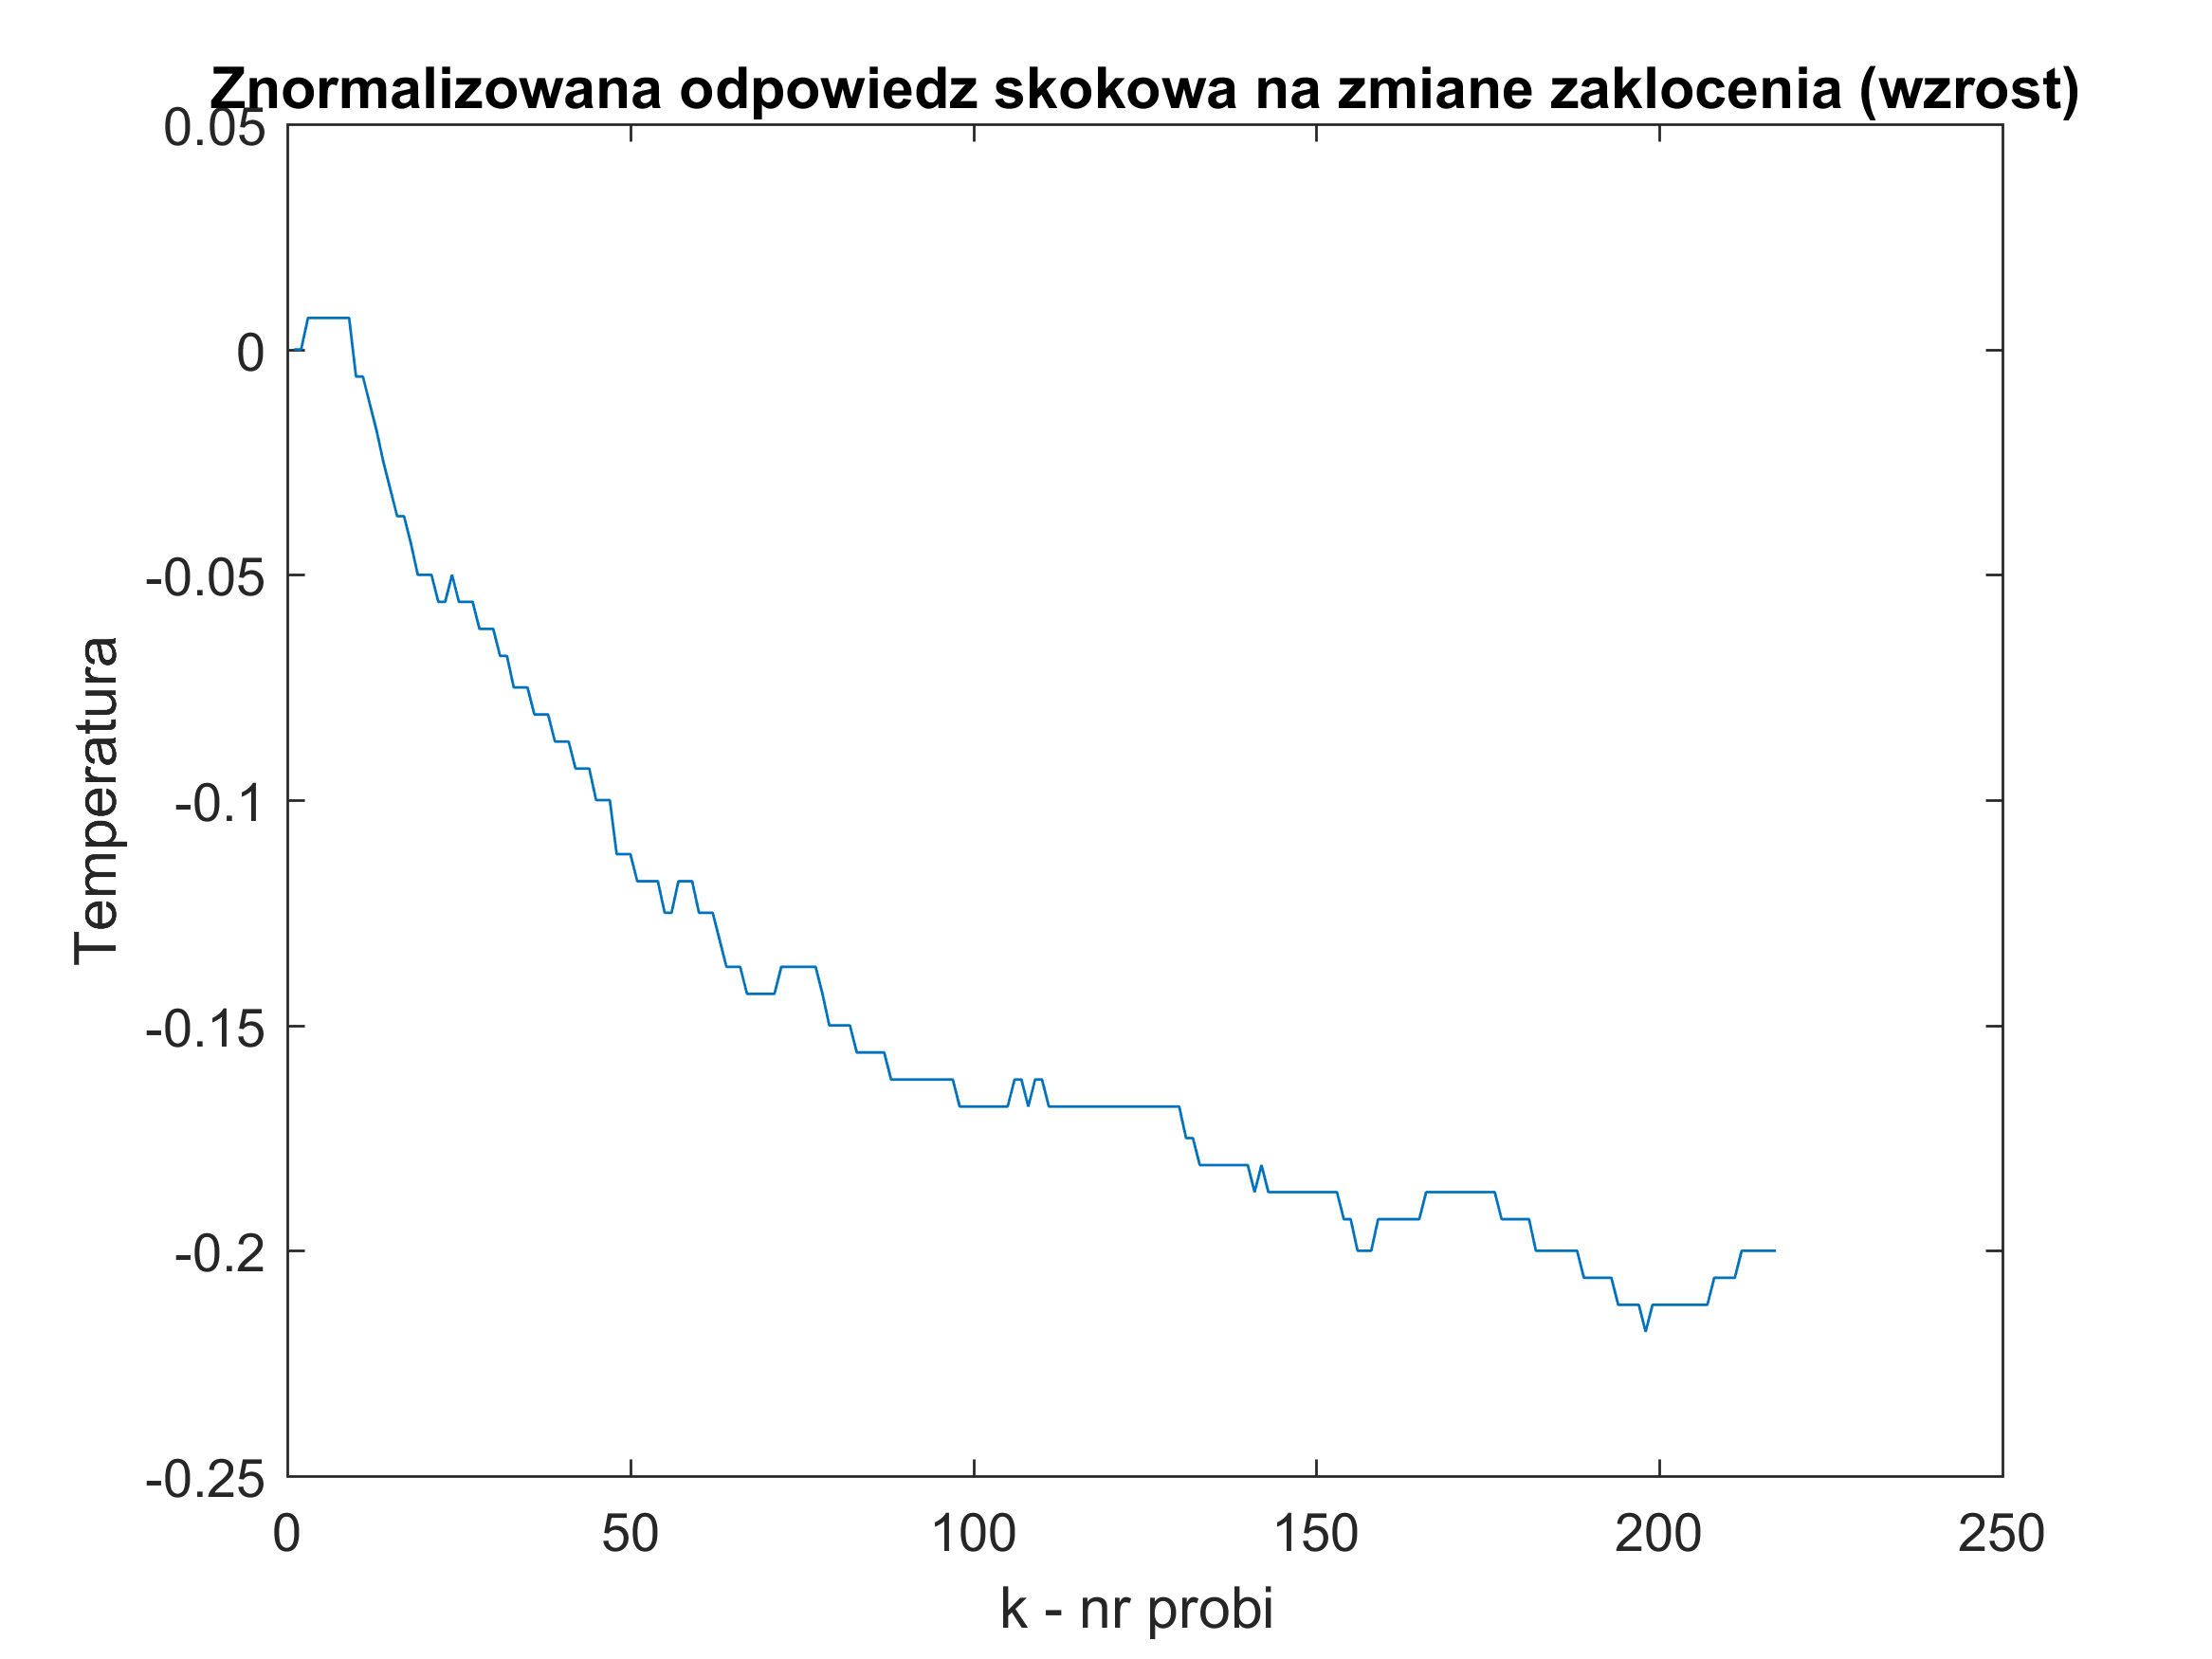
\includegraphics[width=0.9\linewidth]{nor_od_skok_wg}
	\caption{Znormalizowana odpowiedź skokowa na zmianę sterowania wentylatorem z $30\%$ na $40\%$}
	\label{fig:noswg}
\end{figure}
\begin{figure}[H]
	\centering
	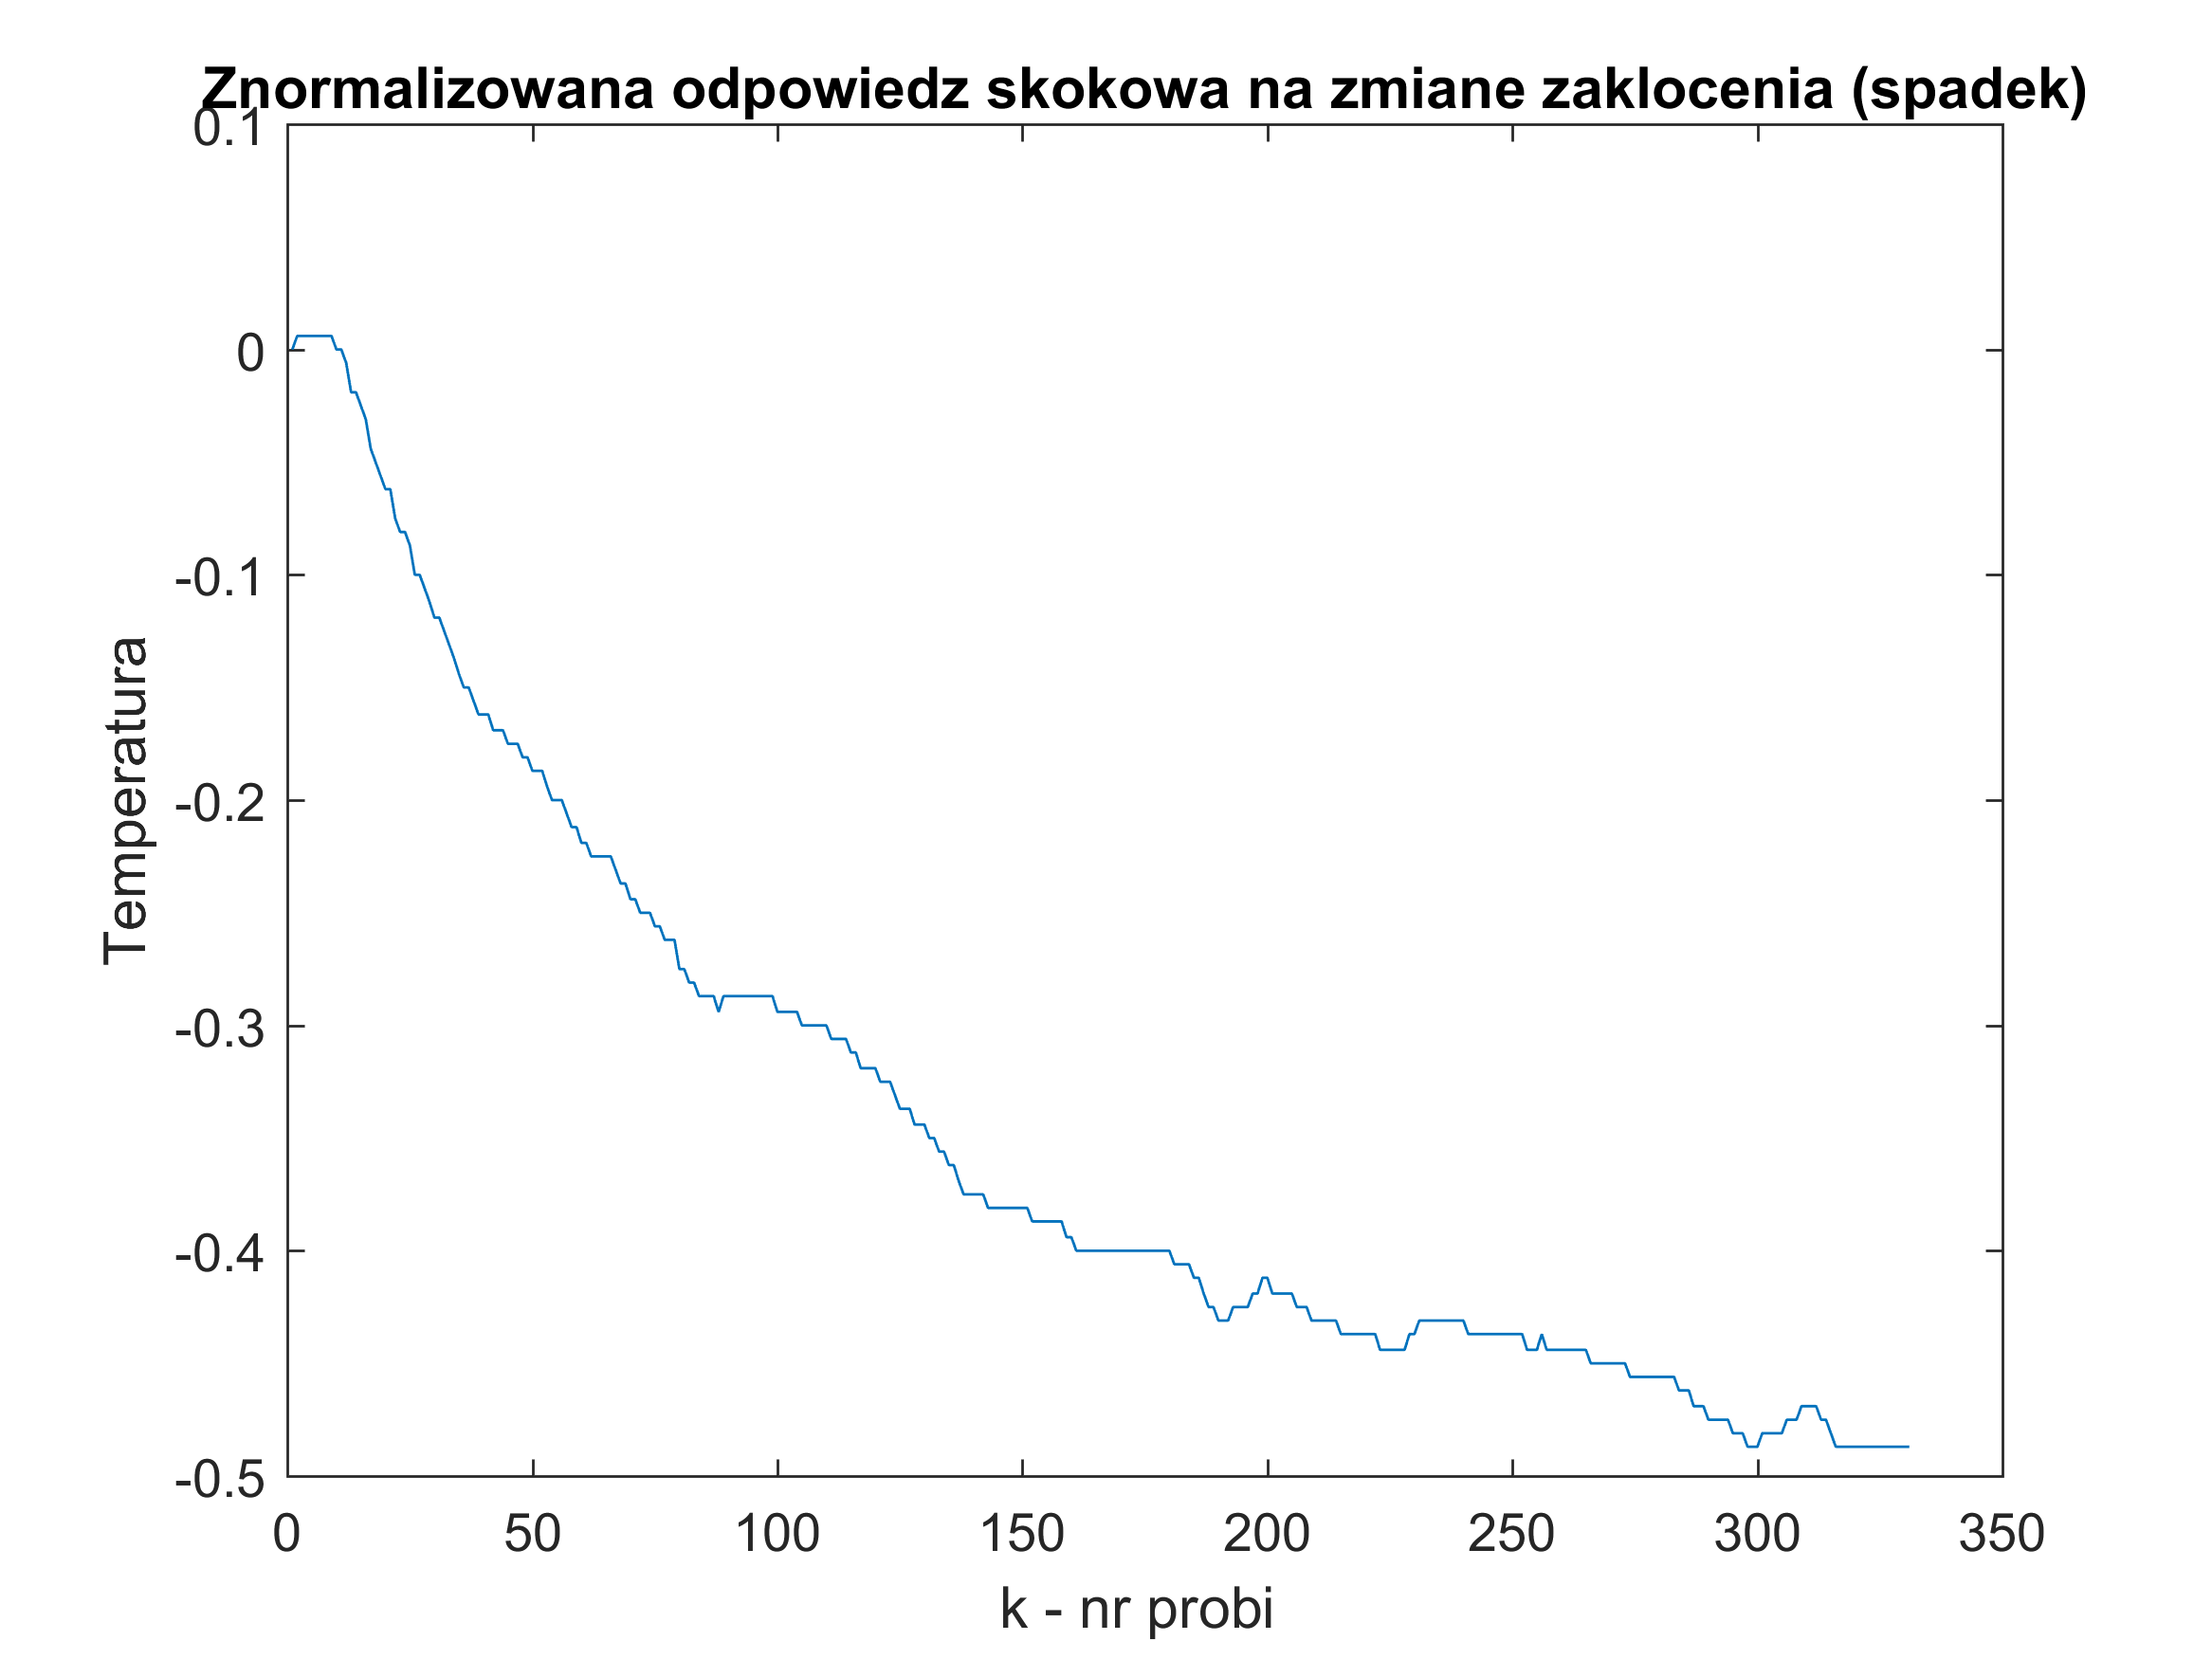
\includegraphics[width=0.9\linewidth]{nor_od_skok_wd}
	\caption{Znormalizowana odpowiedź skokowa na zmianę sterowania wentylatorem z $30\%$ na $20\%$}
	\label{fig:noswd}
\end{figure}
Już z wykresów \ref{fig:noswd} i \ref{fig:noswg} wynika, że zakłócenie w sposób nieliniowy wpływa na stanowisko - osiągane są chociażby znacząco różniące się od siebie wzmocnienia. Aby nie wprowadzać dodatkowych komplikacji w strukturze sterowania, podjeliśmy decyzję o wykorzystaniu tylko jednej transmitancji do odprzęgania zakłóceń. Transmitancja ta będzie kompromisem pomiędzy dwoma obliczonymi modelami. 
Podobnie jak w punkcie \ref{grzalka} zauważyliśmy, że przebiegi sygnałów przypominają odpowiedź skokową obiektu z jedną inercją. Z tego powodu także w tym punkcie wykorzystaliśmy idetyfikację metodą graficzną.\\
Dla zmiany sygnału sterującego wentylatorem z $30\%$ na $40\%$ odczytane zostały następujące wartości parametrów modelu:
\[\tau=8\]
\[K=-0,21\]
\[T_{0}=62\]
Transmitancja ta wystarczająco dobrze opisuje model przy wzroście zakłóceń, dlatego nie była konieczna dalsza modyfikacja parametrów.

Na wykresie \ref{fig:transmi_wg} przedstawiony został przebieg odpowiedzi skokowych modeli z obliczonymi transmitancjami oraz znormalizowanej odpowiedzi skokowej zebranej z obiektu.
\begin{figure}[H]
	\centering
	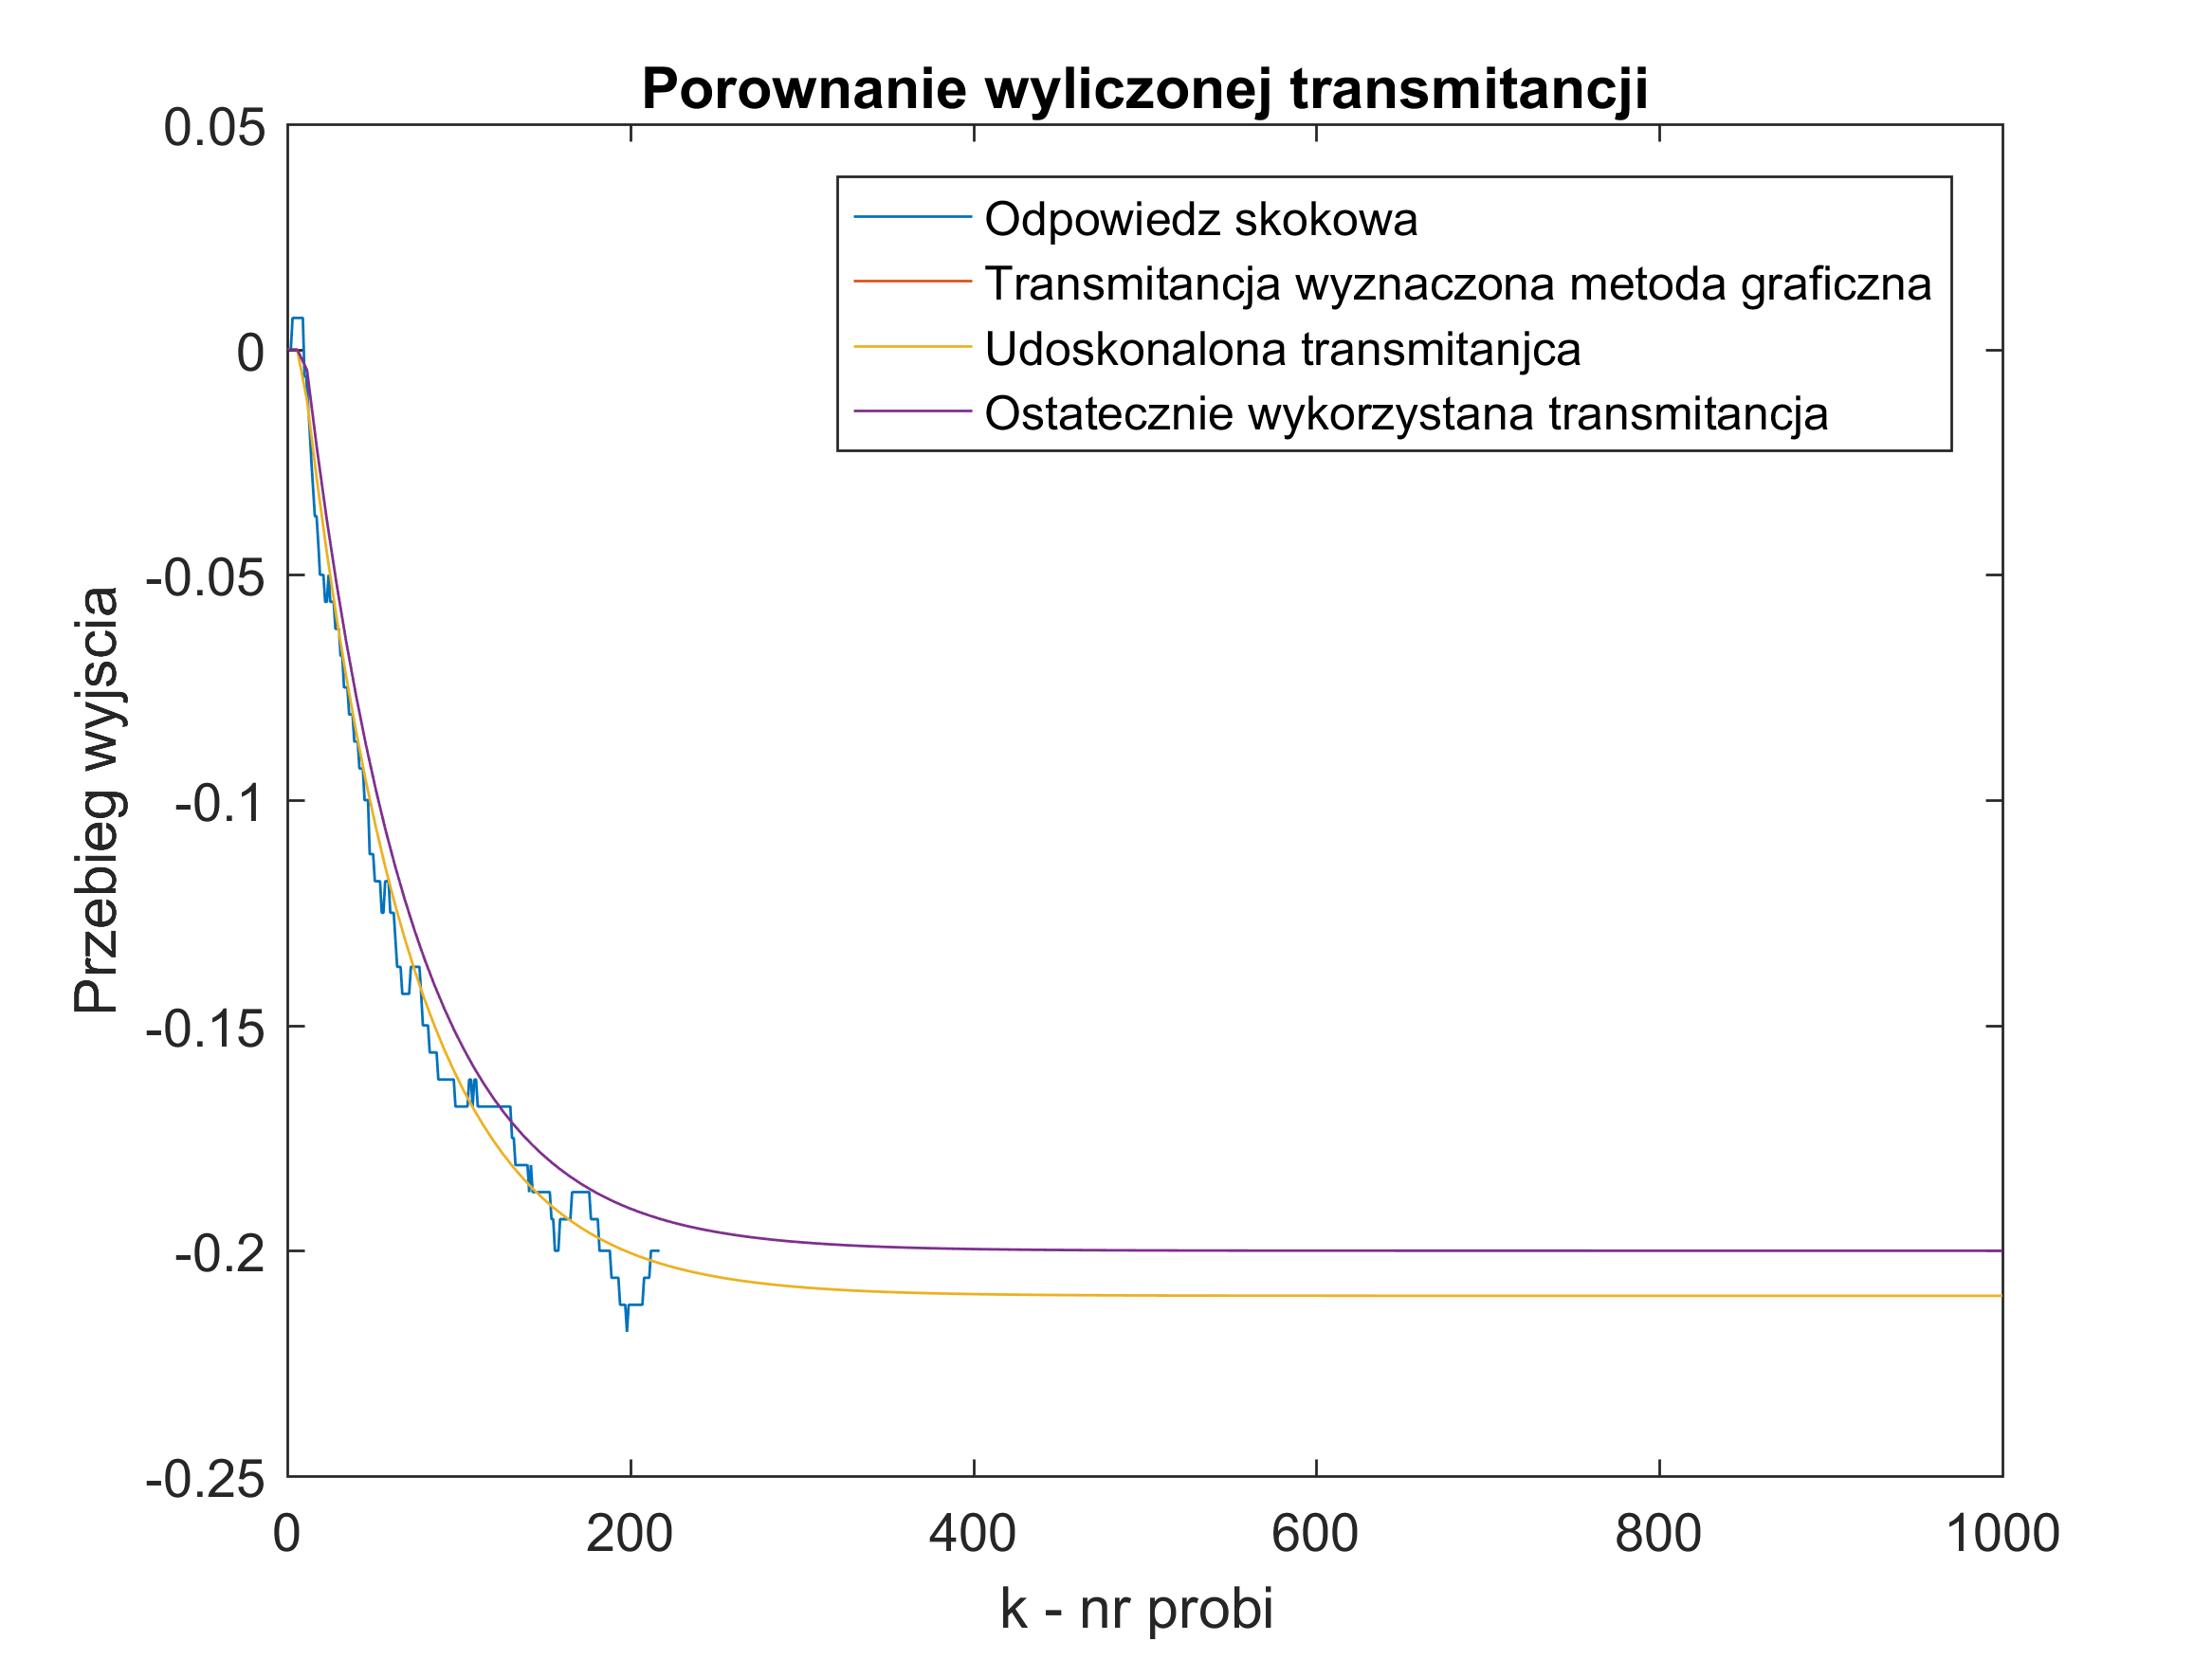
\includegraphics[width=0.9\linewidth]{transmi_wg}
	\caption  {Porównanie przebiegów odpowiedzi skokowej i obliczonych transmitancji}
	\label{fig:transmi_wg}
\end{figure}
Dla zmiany sygnału sterującego wentylatorem z $30\%$ na $20\%$ odczytane zostały następujące wartości parametrów modelu:
\[\tau=10\]
\[K=-0,487\]
\[T_{0}=104\]
W tym przypadku zamodelowany sygnał za bardzo odbiega od uzyskanej odpowiedzi skokowej z obiektu, dlatego dokonane zostały następujące modyfikacje parametrów modelu:
\[\tau=10\]
\[K=-0,487\]
\[T_{0}=85\]

Na wykresie \ref{fig:transmi_wdlep} przedstawiony został przebieg odpowiedzi skokowych modeli oraz znormalizowanej odpowiedzi skokowej zebranej z obiektu.
\begin{figure}[H]
	\centering
	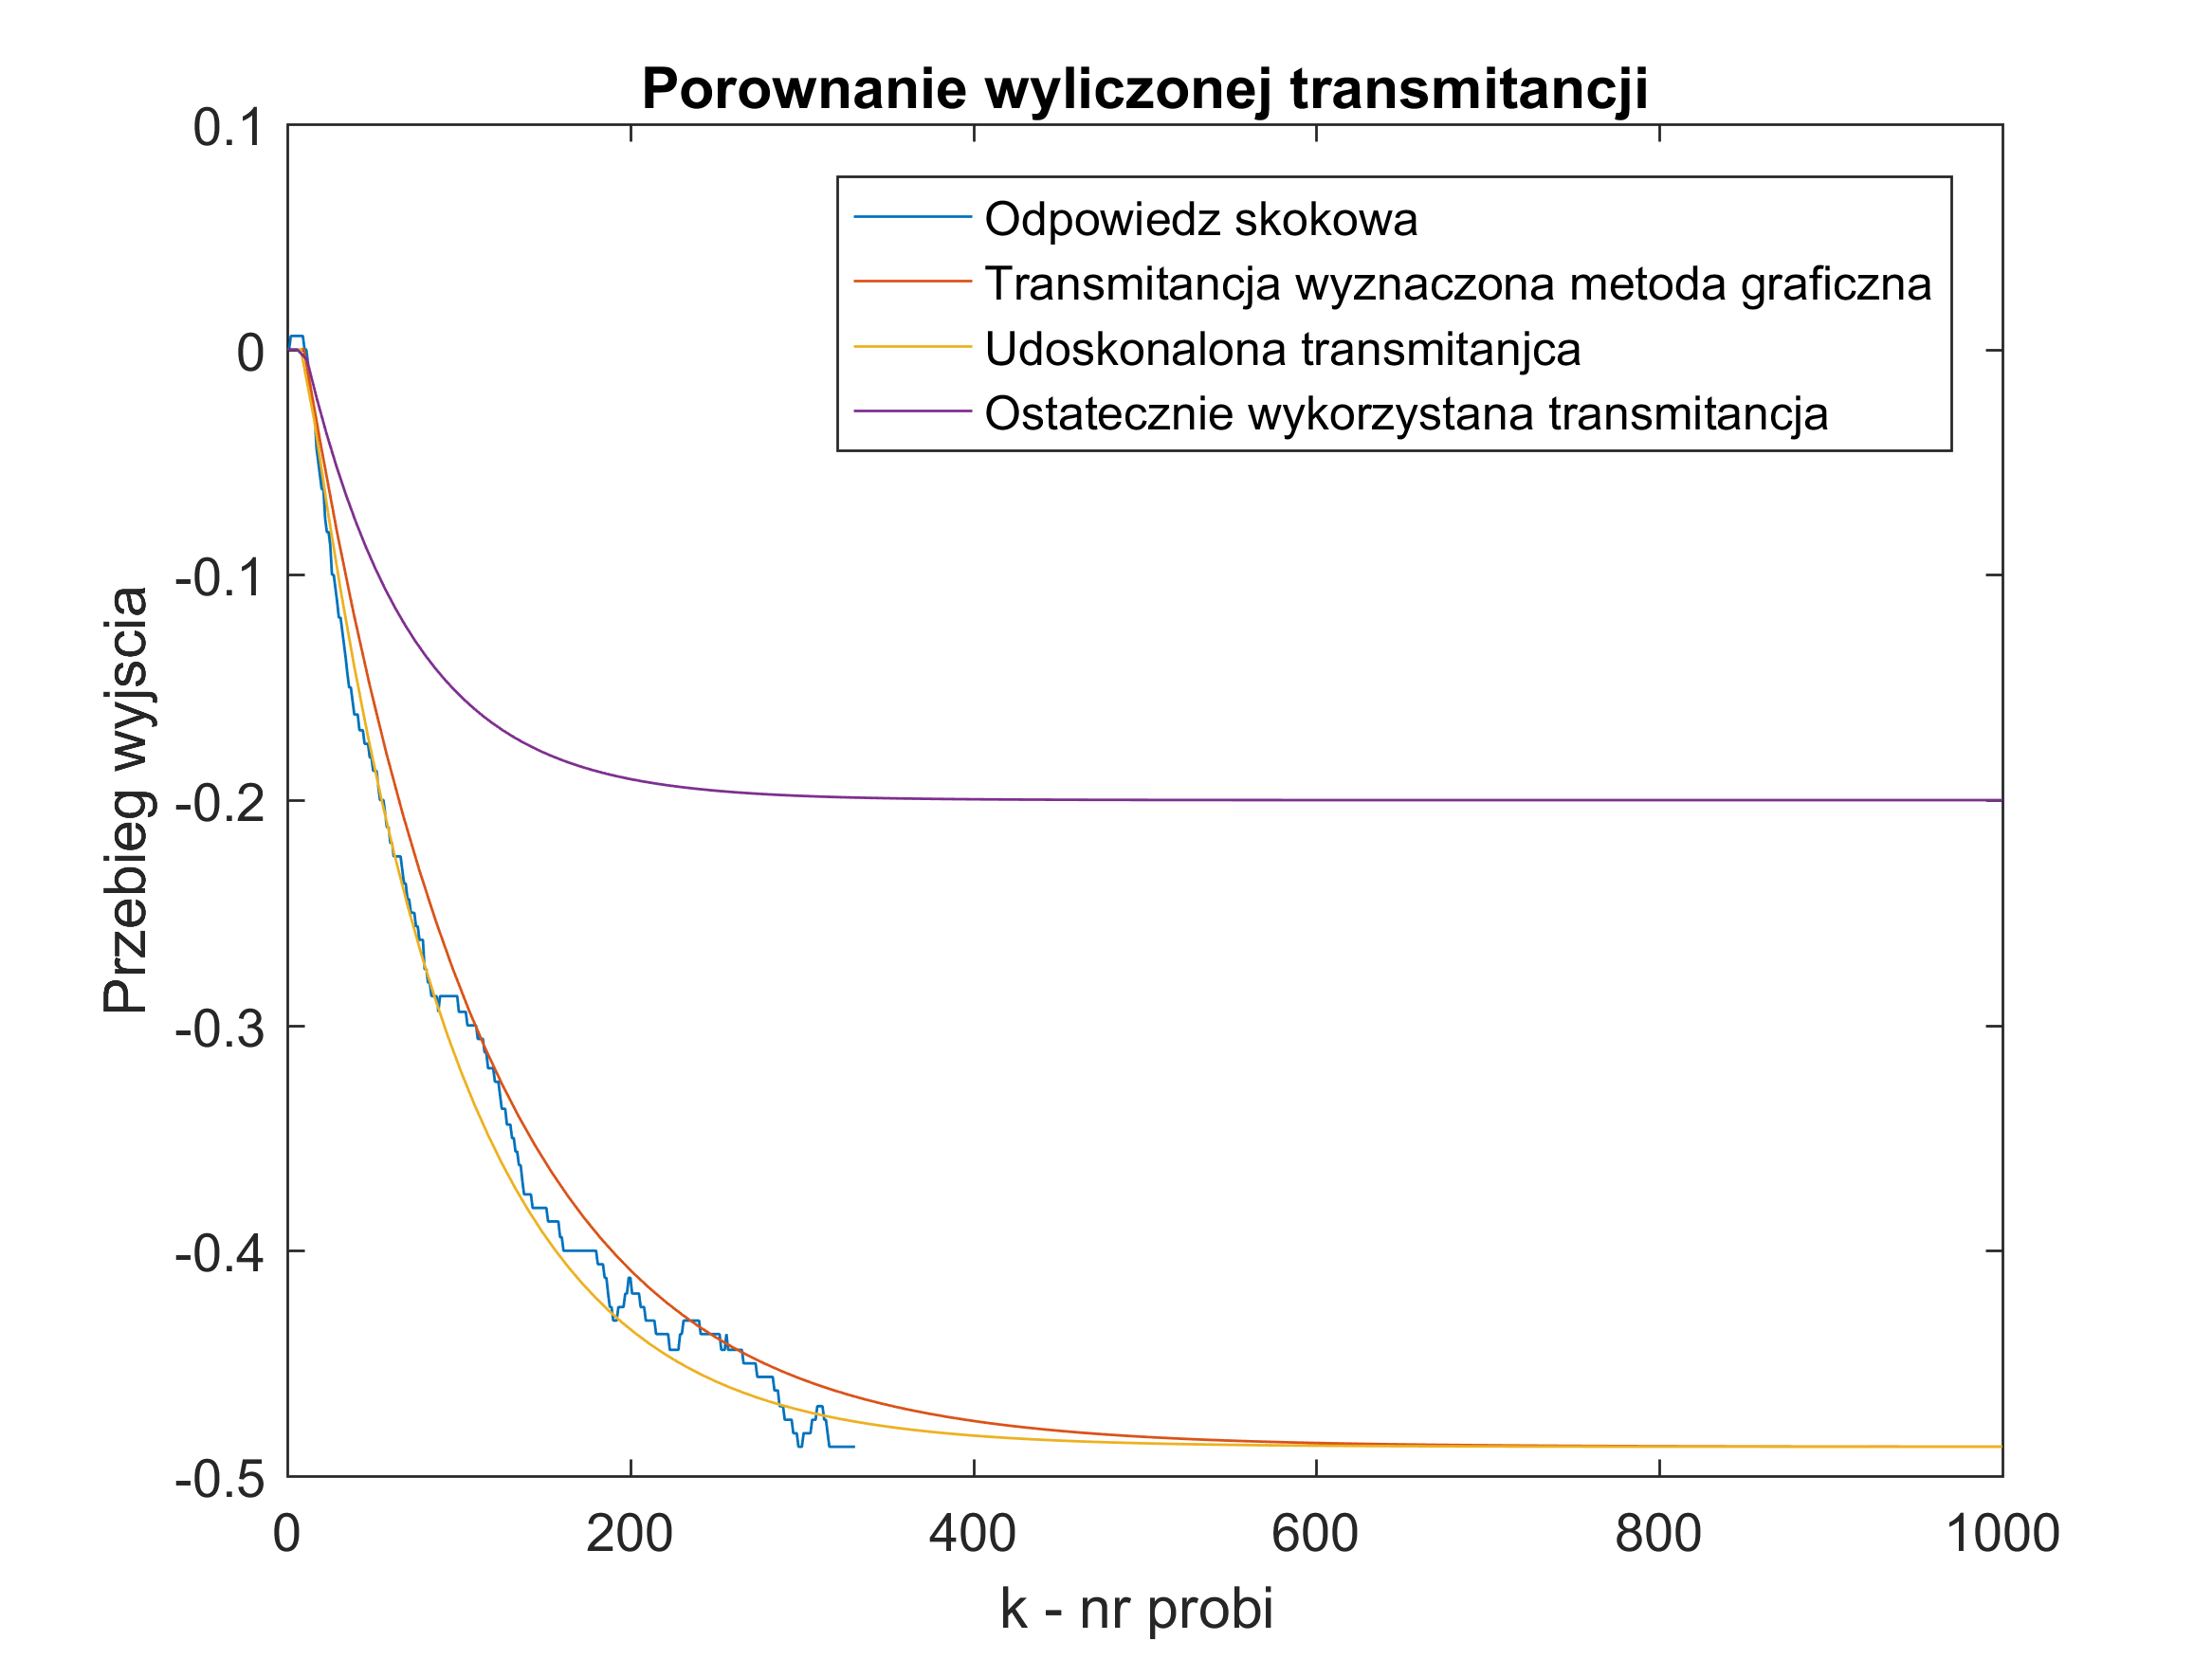
\includegraphics[width=0.9\linewidth]{transmi_wdlep}
	\caption  {Porównanie przebiegów odpowiedzi skokowej i obliczonych transmitancji}
	\label{fig:transmi_wdlep}
\end{figure}
Po przeprowadzeniu eksperymentów testujących działanie członu odprzęgającego zauważyliśmy, że zakłócenia są najlepiej redukowane dla następujących parametrów transmitancji zakłóceń:
\[\tau=10\]
\[K=-0,2\]
\[T_{0}=62\]
Jest ona zaznaczona na wykresach \ref{fig:transmi_wg} i \ref{fig:transmi_wdlep} kolorem filoteowym.
Wzór na ostatecznie wykorzystywaną transmitancję zakłóceń ma postać:
\[T_{Z}(s)=e^{-10 \cdot s} \cdot \frac{-0,2}{62 \cdot s +1}\]


\section{Struktura}
Głównym zadaniem było stworzenie aplikacji sterujacej obiektem grzejąco-chłodzącym w systemie DCS. Naszym zadaniem było sterowanie obiektem o jednym wejściu - temperatury T1, jednym wyjściu - sterowanie grzałki G1 i jednym zaklóceniu - wentylator W1. Należało zaimplementować pętlę regulacji z regulatorem PID i członem odprzęgającym, która powoduje, że obiekt dąży do zadanej temperatury i eliminuje wpływ zakłócenia wentylatora W1. Komunikacja z obiektem odbywała się przez MODBUS. 

Naszym zadaniem było stworzenie logiki w Control Builderze (Rysunek \ref{fig:schemat}). Przyjmuje ona jako wejścia:\\
- aktualną temperaturę jako wejście sterowalne obiektu (ST1 MODBUS TEMP1)\\
- aktualne sterowanie wentylatora jako zakłocenie mierzalne (ST1 MODBUS FAN4)\\
- aktualne sterowanie grzałki - tylko do obserwacji sygnału sterującego (ST1 MODBUS HEATER1)\\
Wyjście z naszej logiki jest wyliczonym sterowaniem grzałki. \\

Przygotowana wcześniej została logika zbierajaca dane z obiektu. Należało w odpowiedni sposób ustawić flagi do bloków typu TRANSFER, żeby wyjście z stworzonej przez nas logiki zostało wysyłane jako aktualne sterowanie grzałki. W tym przygotowanym skrypcie zmienialiśmy także wartość zakłócenia.

Na rysunku \ref{fig:schemat} znajduje się zaimplementowana przez nas pętla regulacji. W Control Builderze programuje się przy pomocy języka FBD. Korzysta się z gotowych bloczków. W programie skorzystaliśmy między innymi z bloków PID, LEAD-LAG, SUM, Avalgen.

Blok PID na wejściu dostawał wartość zadana temperatury (STPT) i wartość aktualnej temperatury T1(CV).  Na rysunku \ref{fig:schemat} jest zaprezentowany schemat logiki z dołączonymi dodatykowymi blokami do ustawiania wartości zadanej, ponieważ jest to schemat zrobiony na potrzeby konkursu (przełączaliśmy wtedy blok DVALGEN, żeby na wejście STPT regulatora PID szła wartośc z przygotowanej przez prowadzącego logiki). W normalnym trybie pracy wartość zadana była ustawiana za pomocą bloku Avalgen.
Aktualna wartość temperatury była pobierana przez punkt ST1 MODBUS TEMP1.

W bloku PID ustawiliśmy nastawy regulatora PID zaprezentowane na rysunku  \ref{fig:12}. Zostały one wyznaczone przy strojeniu regulatora PID w Matlabie, a następnie dopracowane przez zmienianie ich w Signal Diagramie.

Wyjście bloku PID to wyznaczone sterowanie. Częścią zadania było także uwzględnienie w pętli regulacji wpływającego na obiekt   zakłócenia - do wyznaczonego w bloku PID sterowania trzeba dodać (blok SUM) odprzęganie zakłócenia.

Aby tego dokonać należy dodać człon odprzęgający za pomocą bloku LEADLAG wyliczający wartość jaką należy odjąć/dodać, żeby wyeliminować wpływ zakłócenia. Jako wejście do bloku LEADLAG dajemy wartość punktu ST1 MODBUS FAN4, czyli aktualne sterowanie wentylatora. (Na rysunku \ref{fig:schemat} do bloku LEADLAG dodajemy wartośc sumy z bloku Avalgen i ST1 MODBUS FAN4 ale wartość dla Avalgena jest ustawiona na 0.) 

Blok LEADLAG zawiera wyliczoną transmitancję ze wzoru $-\frac{T_z}{T_0}$, gdzie $T_z$ to transmitancja zakłócenia, a $T_0$ to transmitancja obiektu. Blok LEADLAG miał nastawy zaprezentowane na rysunku \ref{fig:12}.

Wyjściem z sumatora (którego wejściami jest wartość z członu odprzęgającego i wartość wyjścia z regulatora) jest sterowanie, które będzie wysłane na obiekt.

\begin{figure}[H]
	\centering
	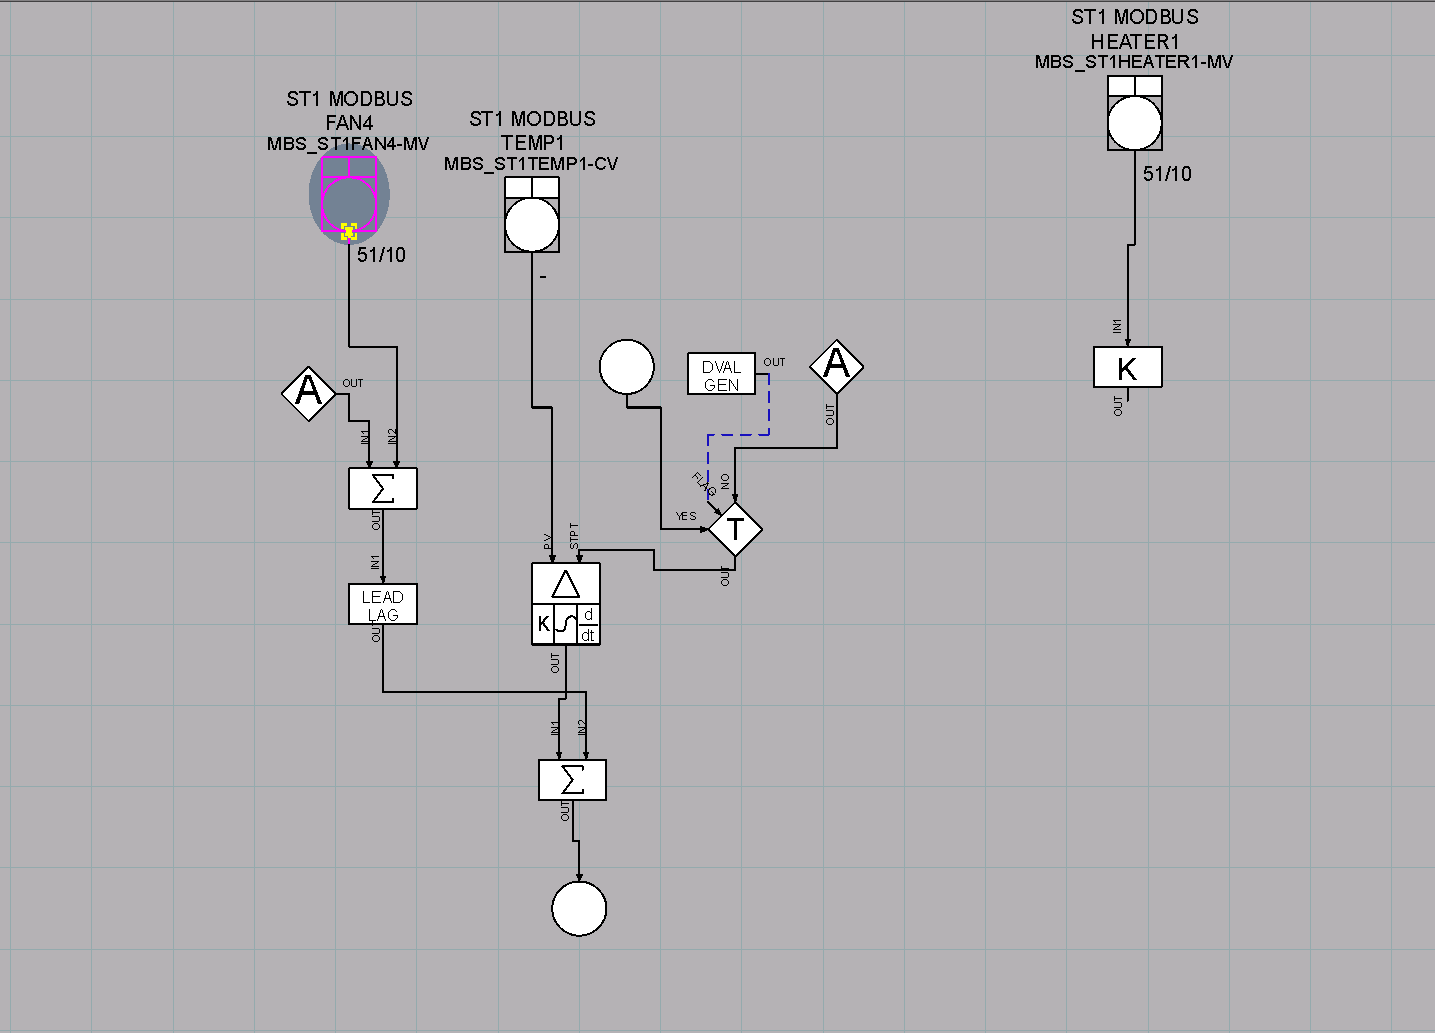
\includegraphics[width=0.9\linewidth]{schemat}
	\caption{Schemat logiki stworzonej w Control Builderze}
	\label{fig:schemat}
\end{figure}

	\begin{figure}[H]
		\centering
		\subfloat[blok PID]{{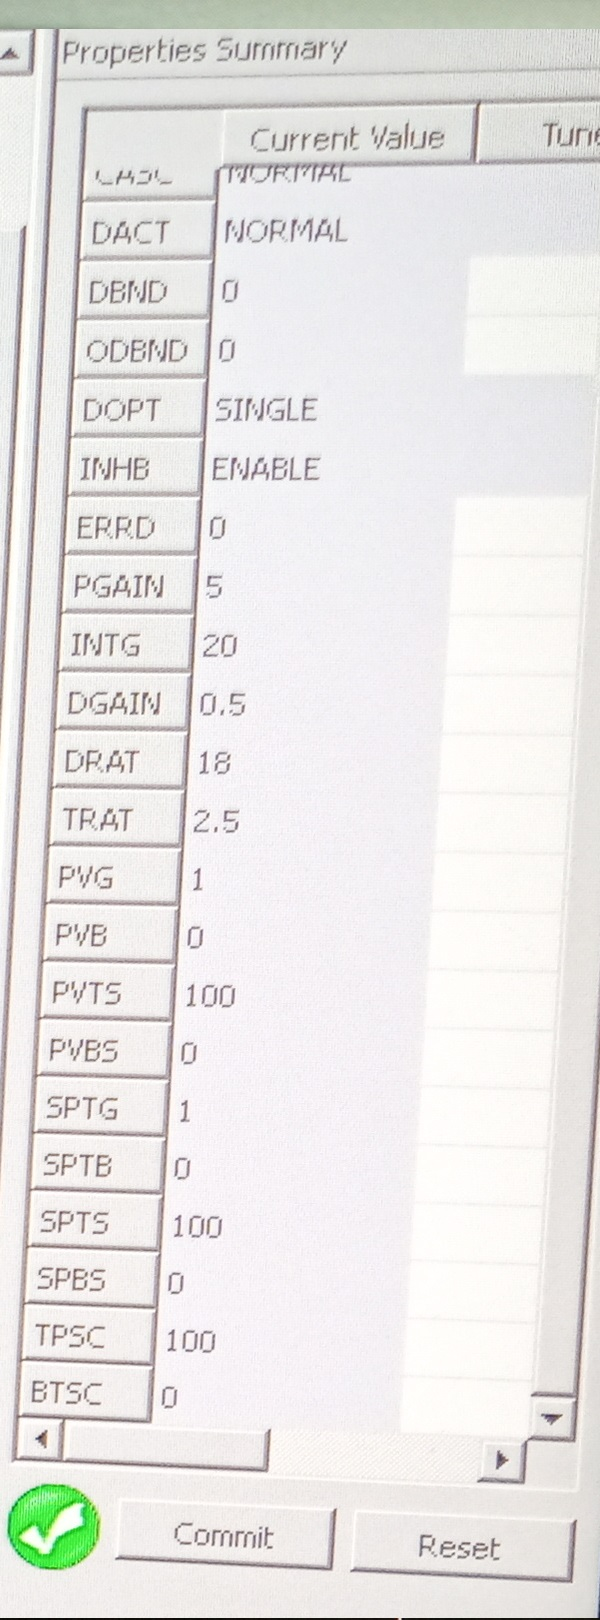
\includegraphics[height=10cm]{1} }}%
		\qquad
		\subfloat[blok LEADLAG odprzęgający zakłócenie]{{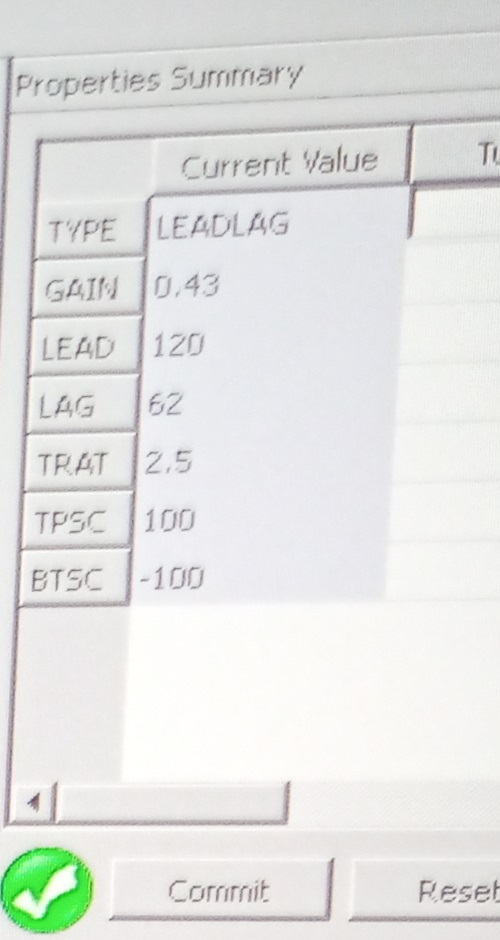
\includegraphics[height=10cm]{2} }}%
		\caption{Nastawy bloków w pętli regulacji}%
		\label{fig:12}%
	\end{figure}


W Control Builderze stworzyliśmy logikę przedstawiona na powyższym rysunku. Następnie uruchomiliśmy ją za pomocą Signal Diagramu i tam zmienialiśmy nastawy regulatora PID i dopracowaliśmy człon odprzęgający. Wartośc zadaną zmienialiśmy w naszej logice w Signal Diagramie, zakłócenie zmieniane było w logice przygotowanej przez prowadzącego także w Signal Diagramie. Za pomocą aplikacji Trend obserwowaliśmy istotne dla nas sygnały (bieżacą temperaturę, zadaną temperaturę, sygnał sterujący grzałką, sygnał sterujący wentylatora).

\section{Strojenie PID}
W pierwszym kroku transmitancje, które uzyskaliśmy dokonując identyfikacji obiketu podczas laboratorium zostały przez nas przekształcone na równania różnicowe. Dzięki temu mogliśmy zaimplementować regulator PID wraz z obiektem i dokonywać symulacji w programie MATLAB. W ten sposób mogliśmy dobrać parametr K, który pozwolił na zadowalającą jakość regulacji. Dobierając wzmocnienie dla regulatora PID człony całkujący i różniczkujący zostały wyłączone. Następnie ulepszając nastawy regulatora postępowaliśmy według zasad metody inżynierskiej, tak żeby wybrane przez nas wskaźniki jakości (czas regulacji, występowanie oscylacji, czas dążenia do wartości zadanej) były optymalne.

Do symulacji regulatora PID użyliśmy udostępnionych nam przez prowadzącego plików. Posłużyliśmy się głównie plikiem \verb|classPID.m| w którym został zaimplementowany regulator PID. Do stworzenia obiektu typu \textit{classPID} używamy konstruktora, który jako argumenty przyjmuje wartości członów regulatora (\textit{classPID(K, Ti, Kd, Td, Tp, Hlim, Llim, Dir, ManVal)}).
 
W celu prezentacji wyników regulacji stworzyliśmy własny skrypt w programie MATLAB. Zadawaliśmy wartość zadaną dla regulatora i obserwowaliśmy jak zachowuje się jego wyjście. Musiało ono jak najszybciej dojść do wartości zadanej i ustabilizować się w krótkim czasie. Dzięki takiej graficznej prezentacji wyników, mogliśmy sprawnie i precyzyjnie dobierać paramtery PID. Wymagane obliczenia do symulacji działania PID były wykonywane na podstawie równań matematycznych opisujących regulator PID w funkcji \textit{calc()}.

Najpierw doprowadziliśmy układ do skraju stabilności objawiało się to niegasnącymi oscylacjami.
\begin{figure}[H]
	\centering
	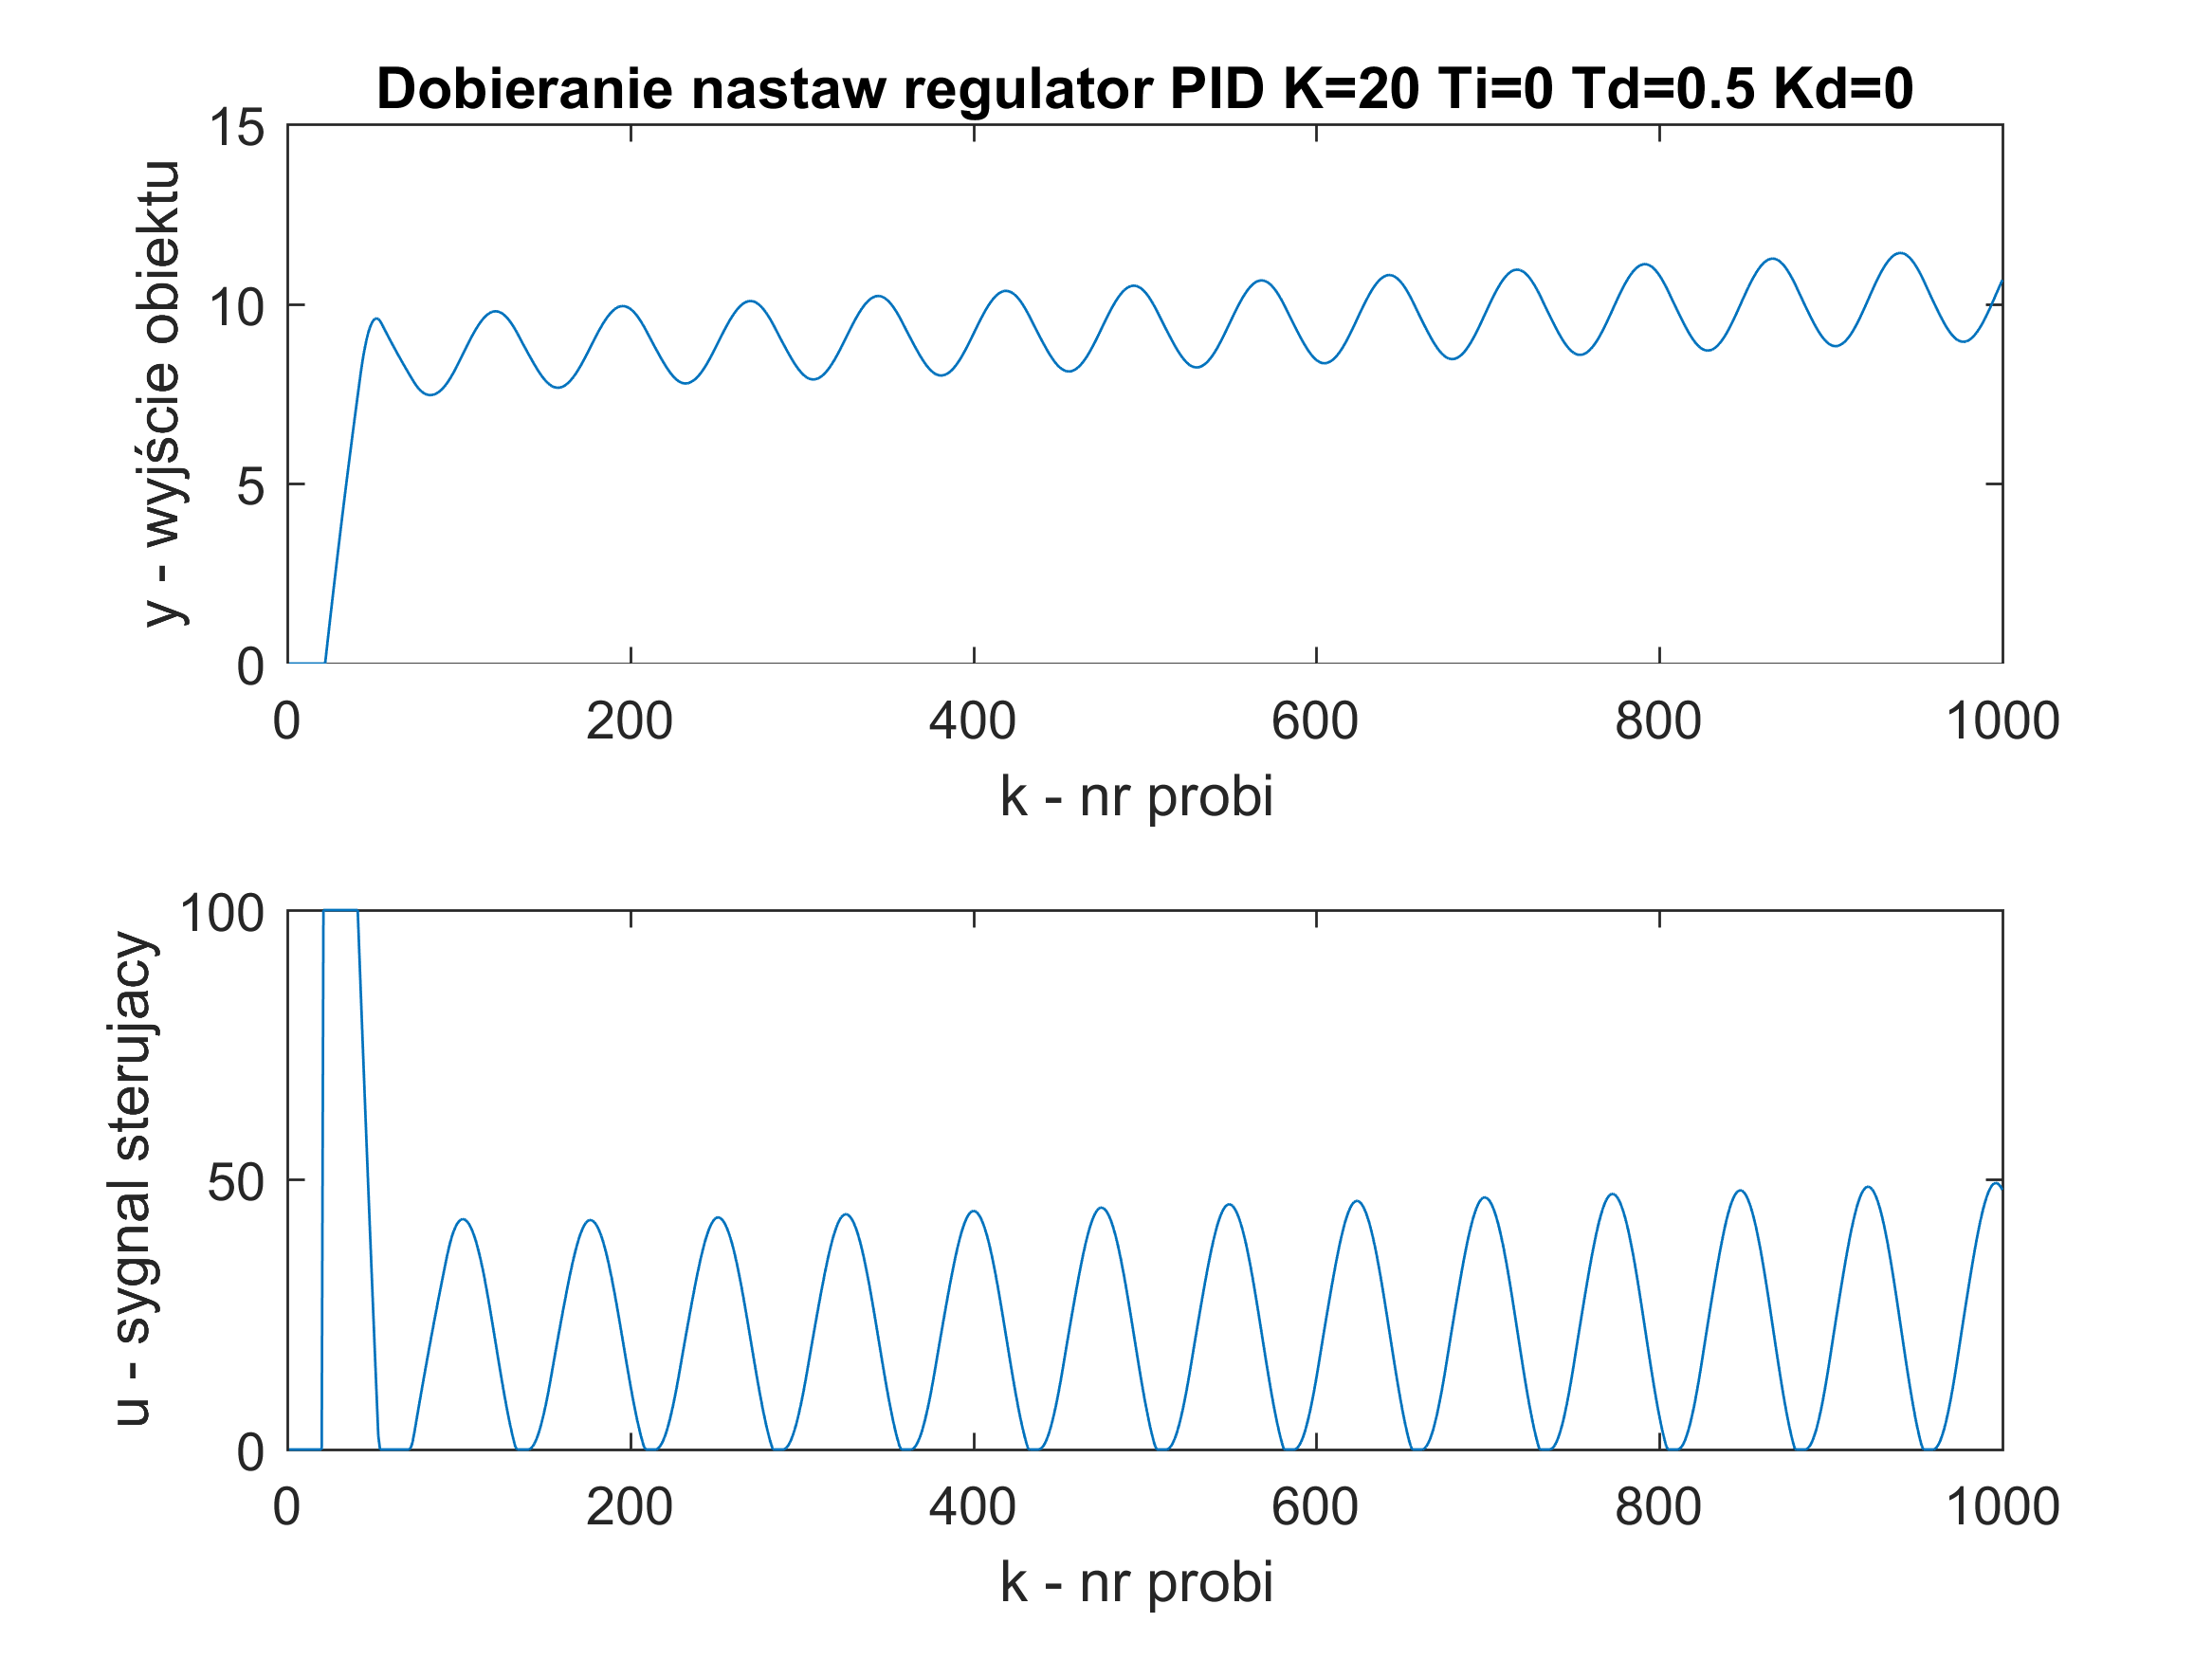
\includegraphics[width=0.9\linewidth]{pid_krytyczny.png}
	\caption{}
\end{figure}
Natępnie po ustawieniu początkowych nastawów szukliśmy wartości dla parametrów dla których jakość regulacji i przebiegi sygnałów były najlepsze. 
\begin{figure}[H]
	\centering
	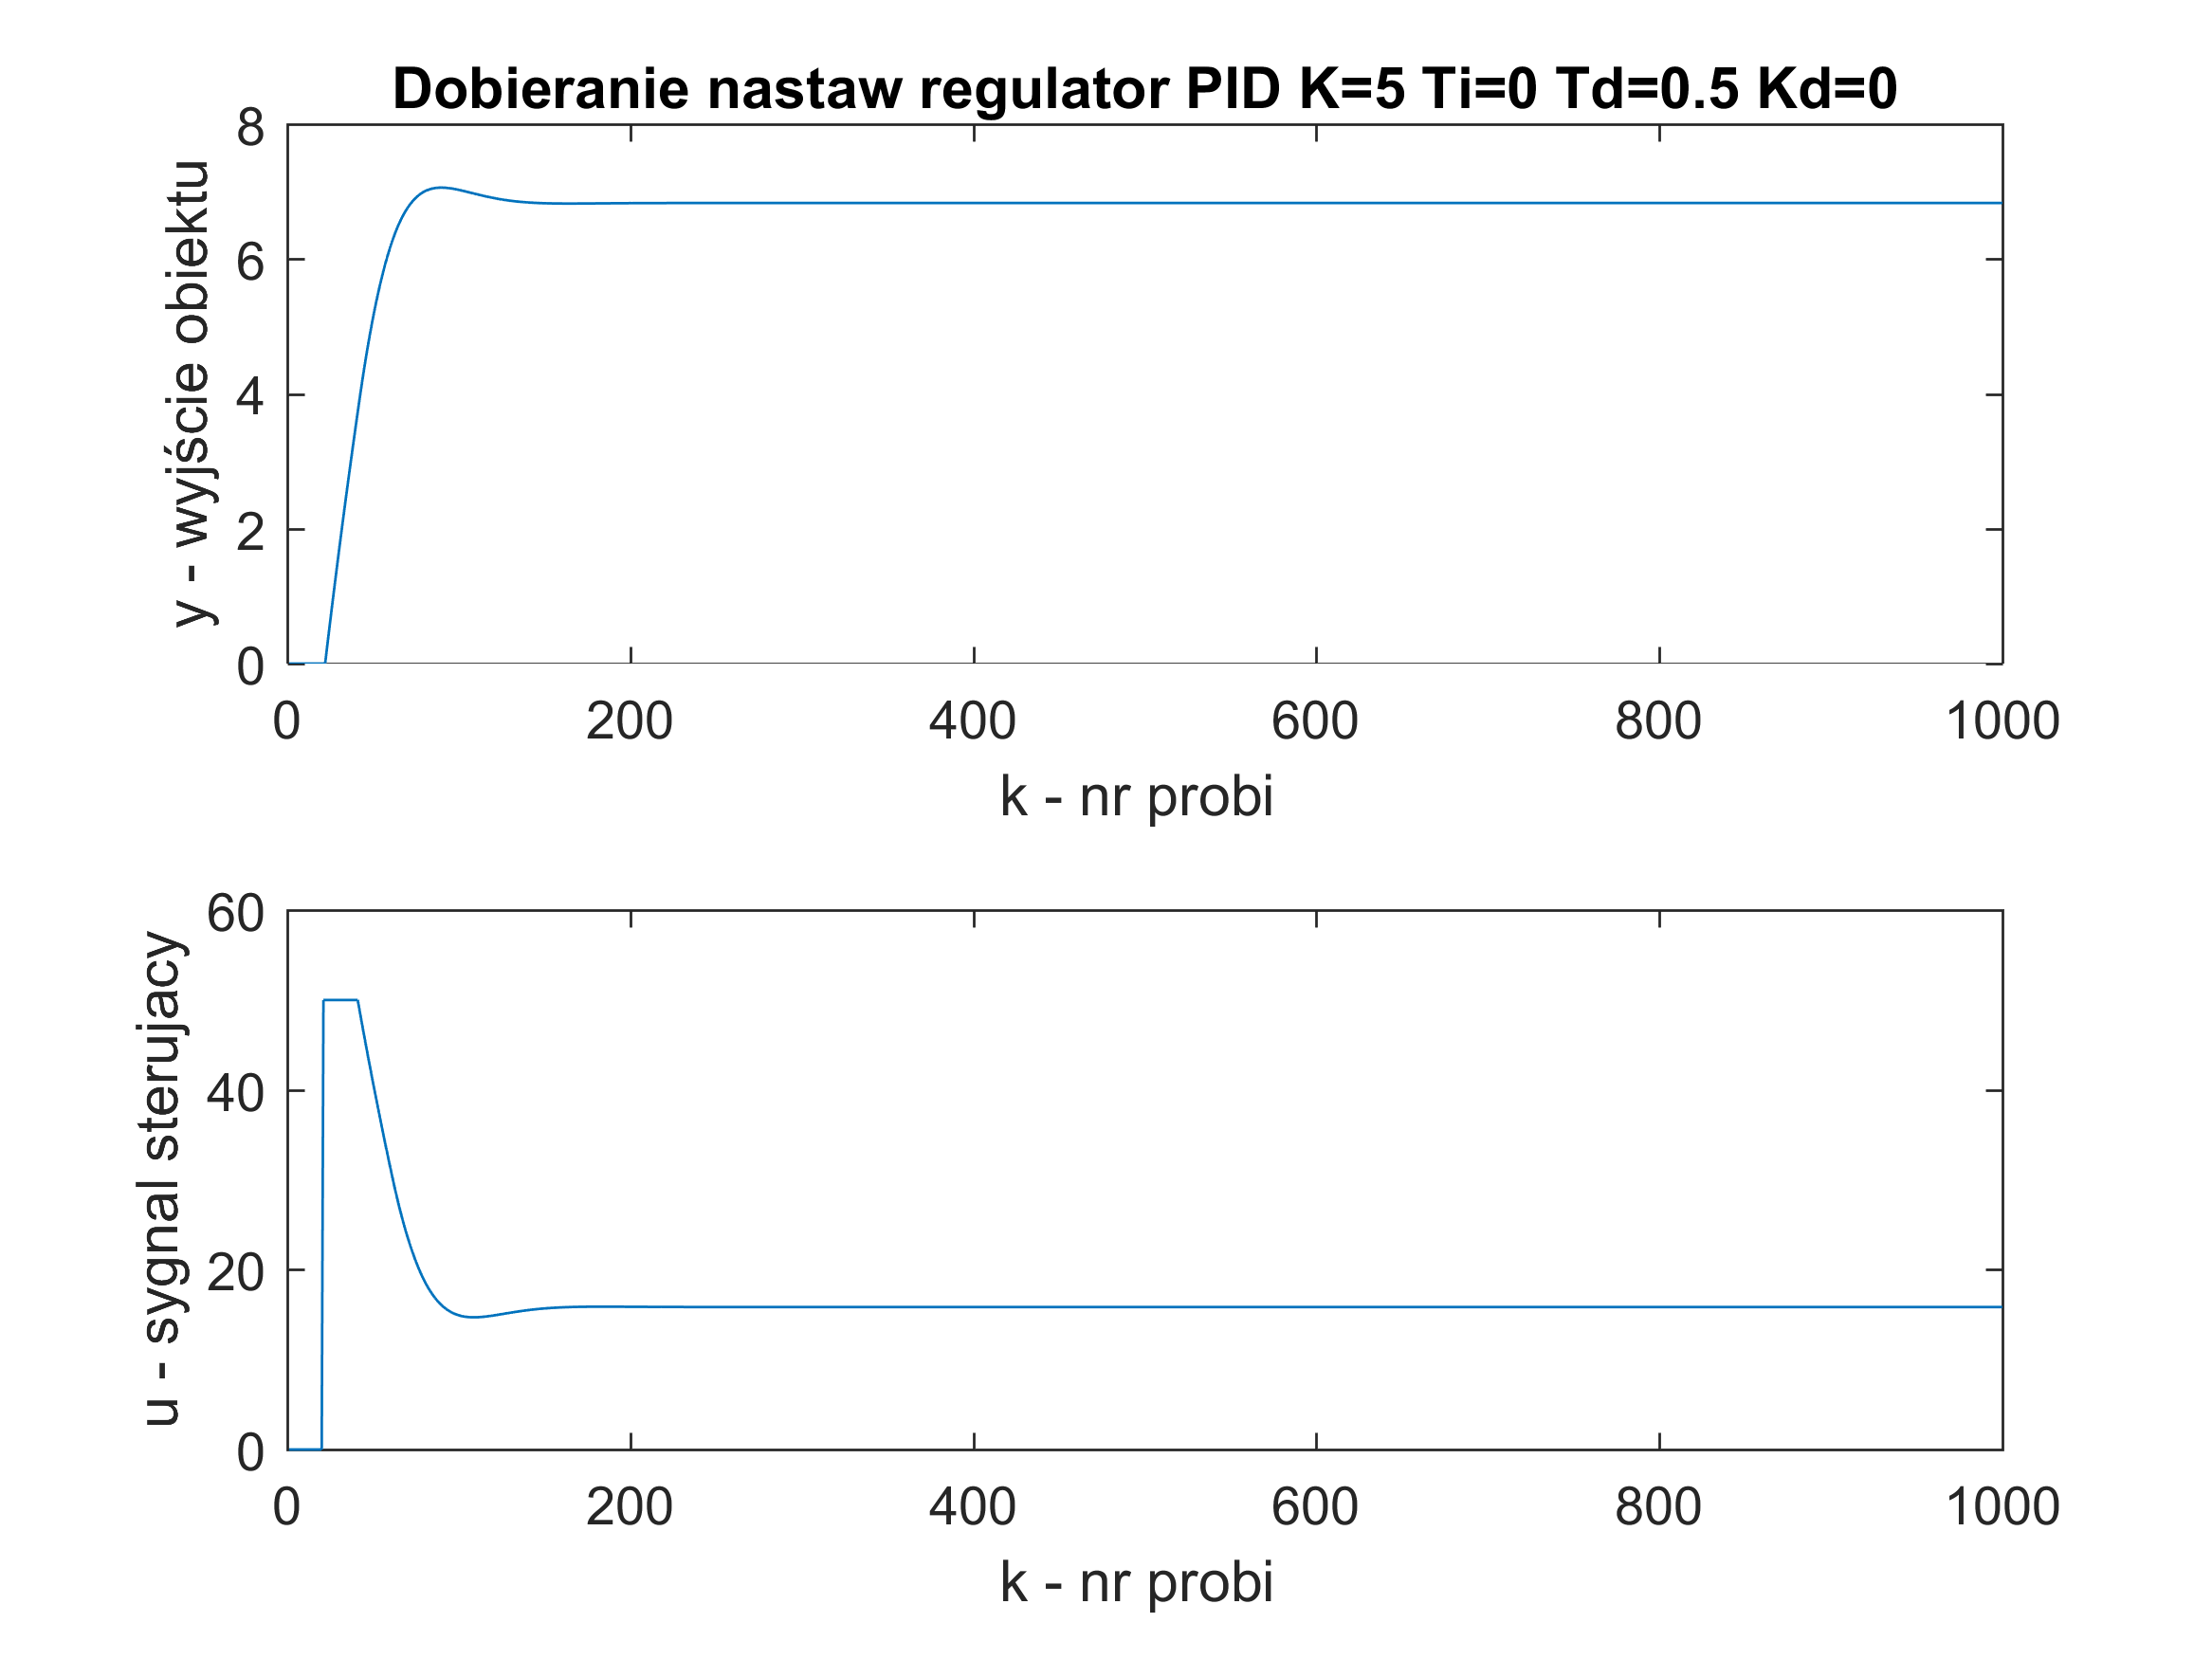
\includegraphics[width=0.9\linewidth]{pid_1.png}
	\caption{}
\end{figure}

\begin{figure}[H]
	\centering
	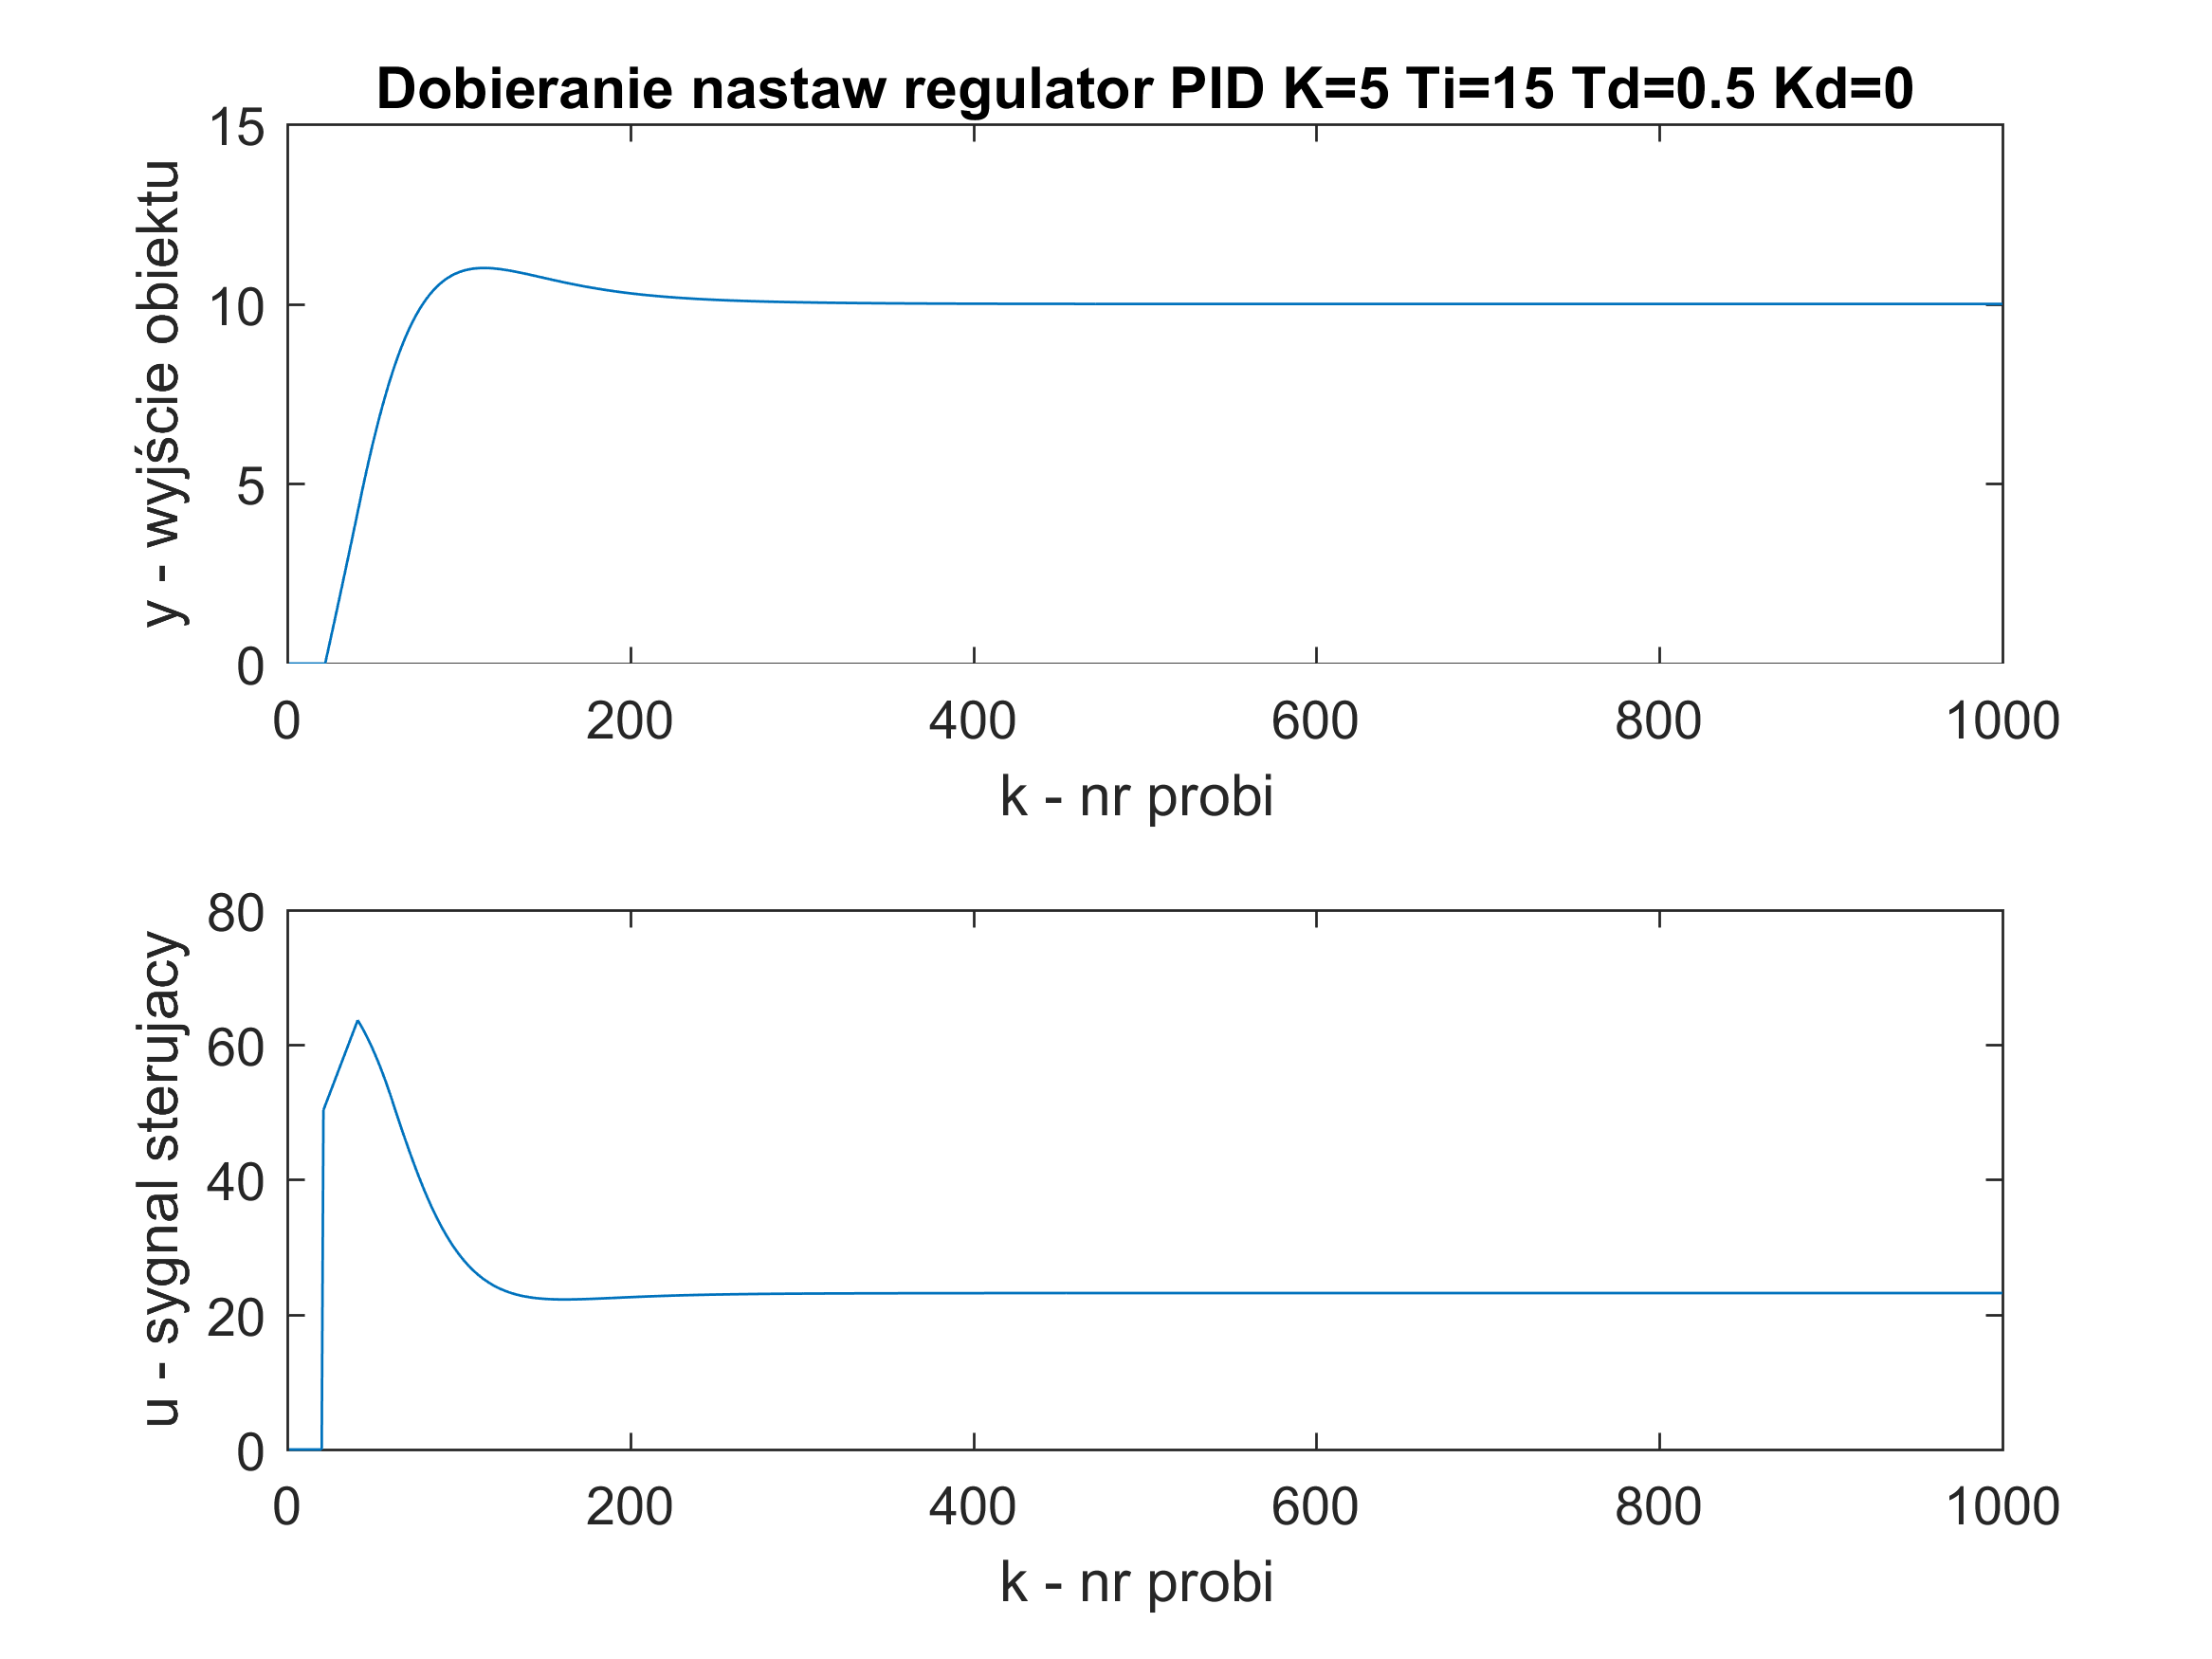
\includegraphics[width=0.9\linewidth]{pid_2.png}
	\caption{}
\end{figure}

\begin{figure}[H]
	\centering
	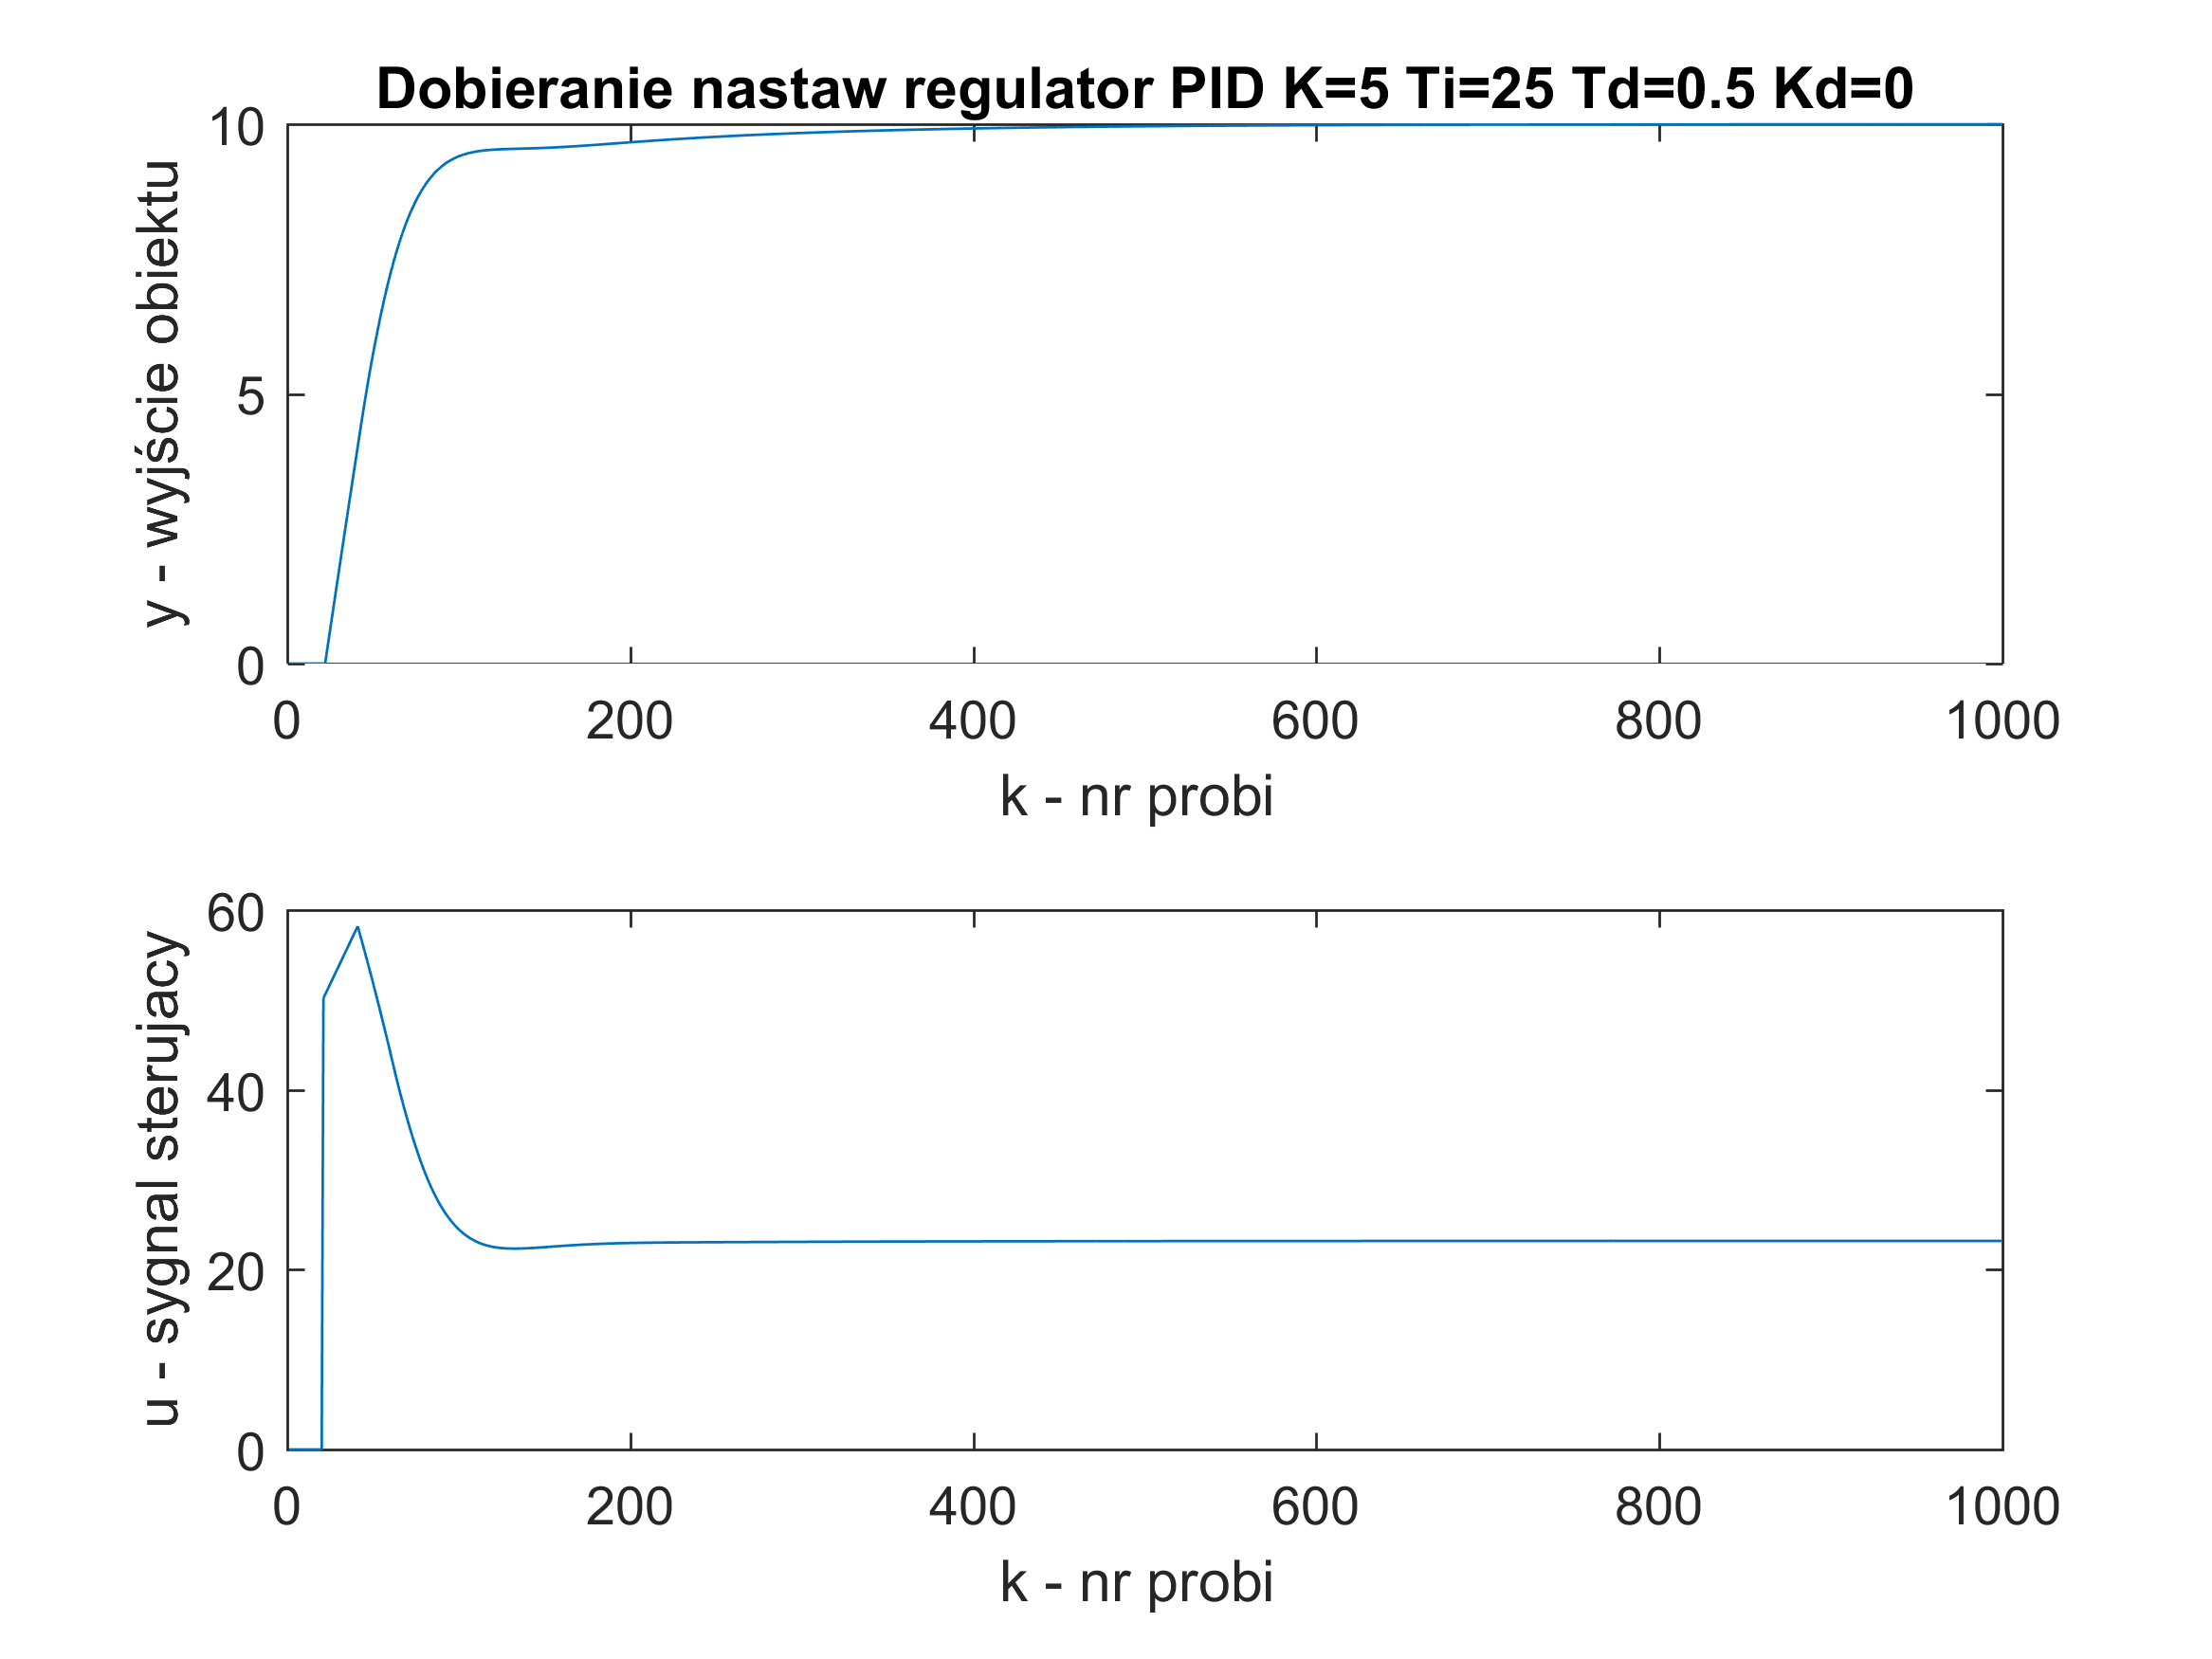
\includegraphics[width=0.9\linewidth]{pid_3.png}
	\caption{}
\end{figure}

\begin{figure}[H]
	\centering
	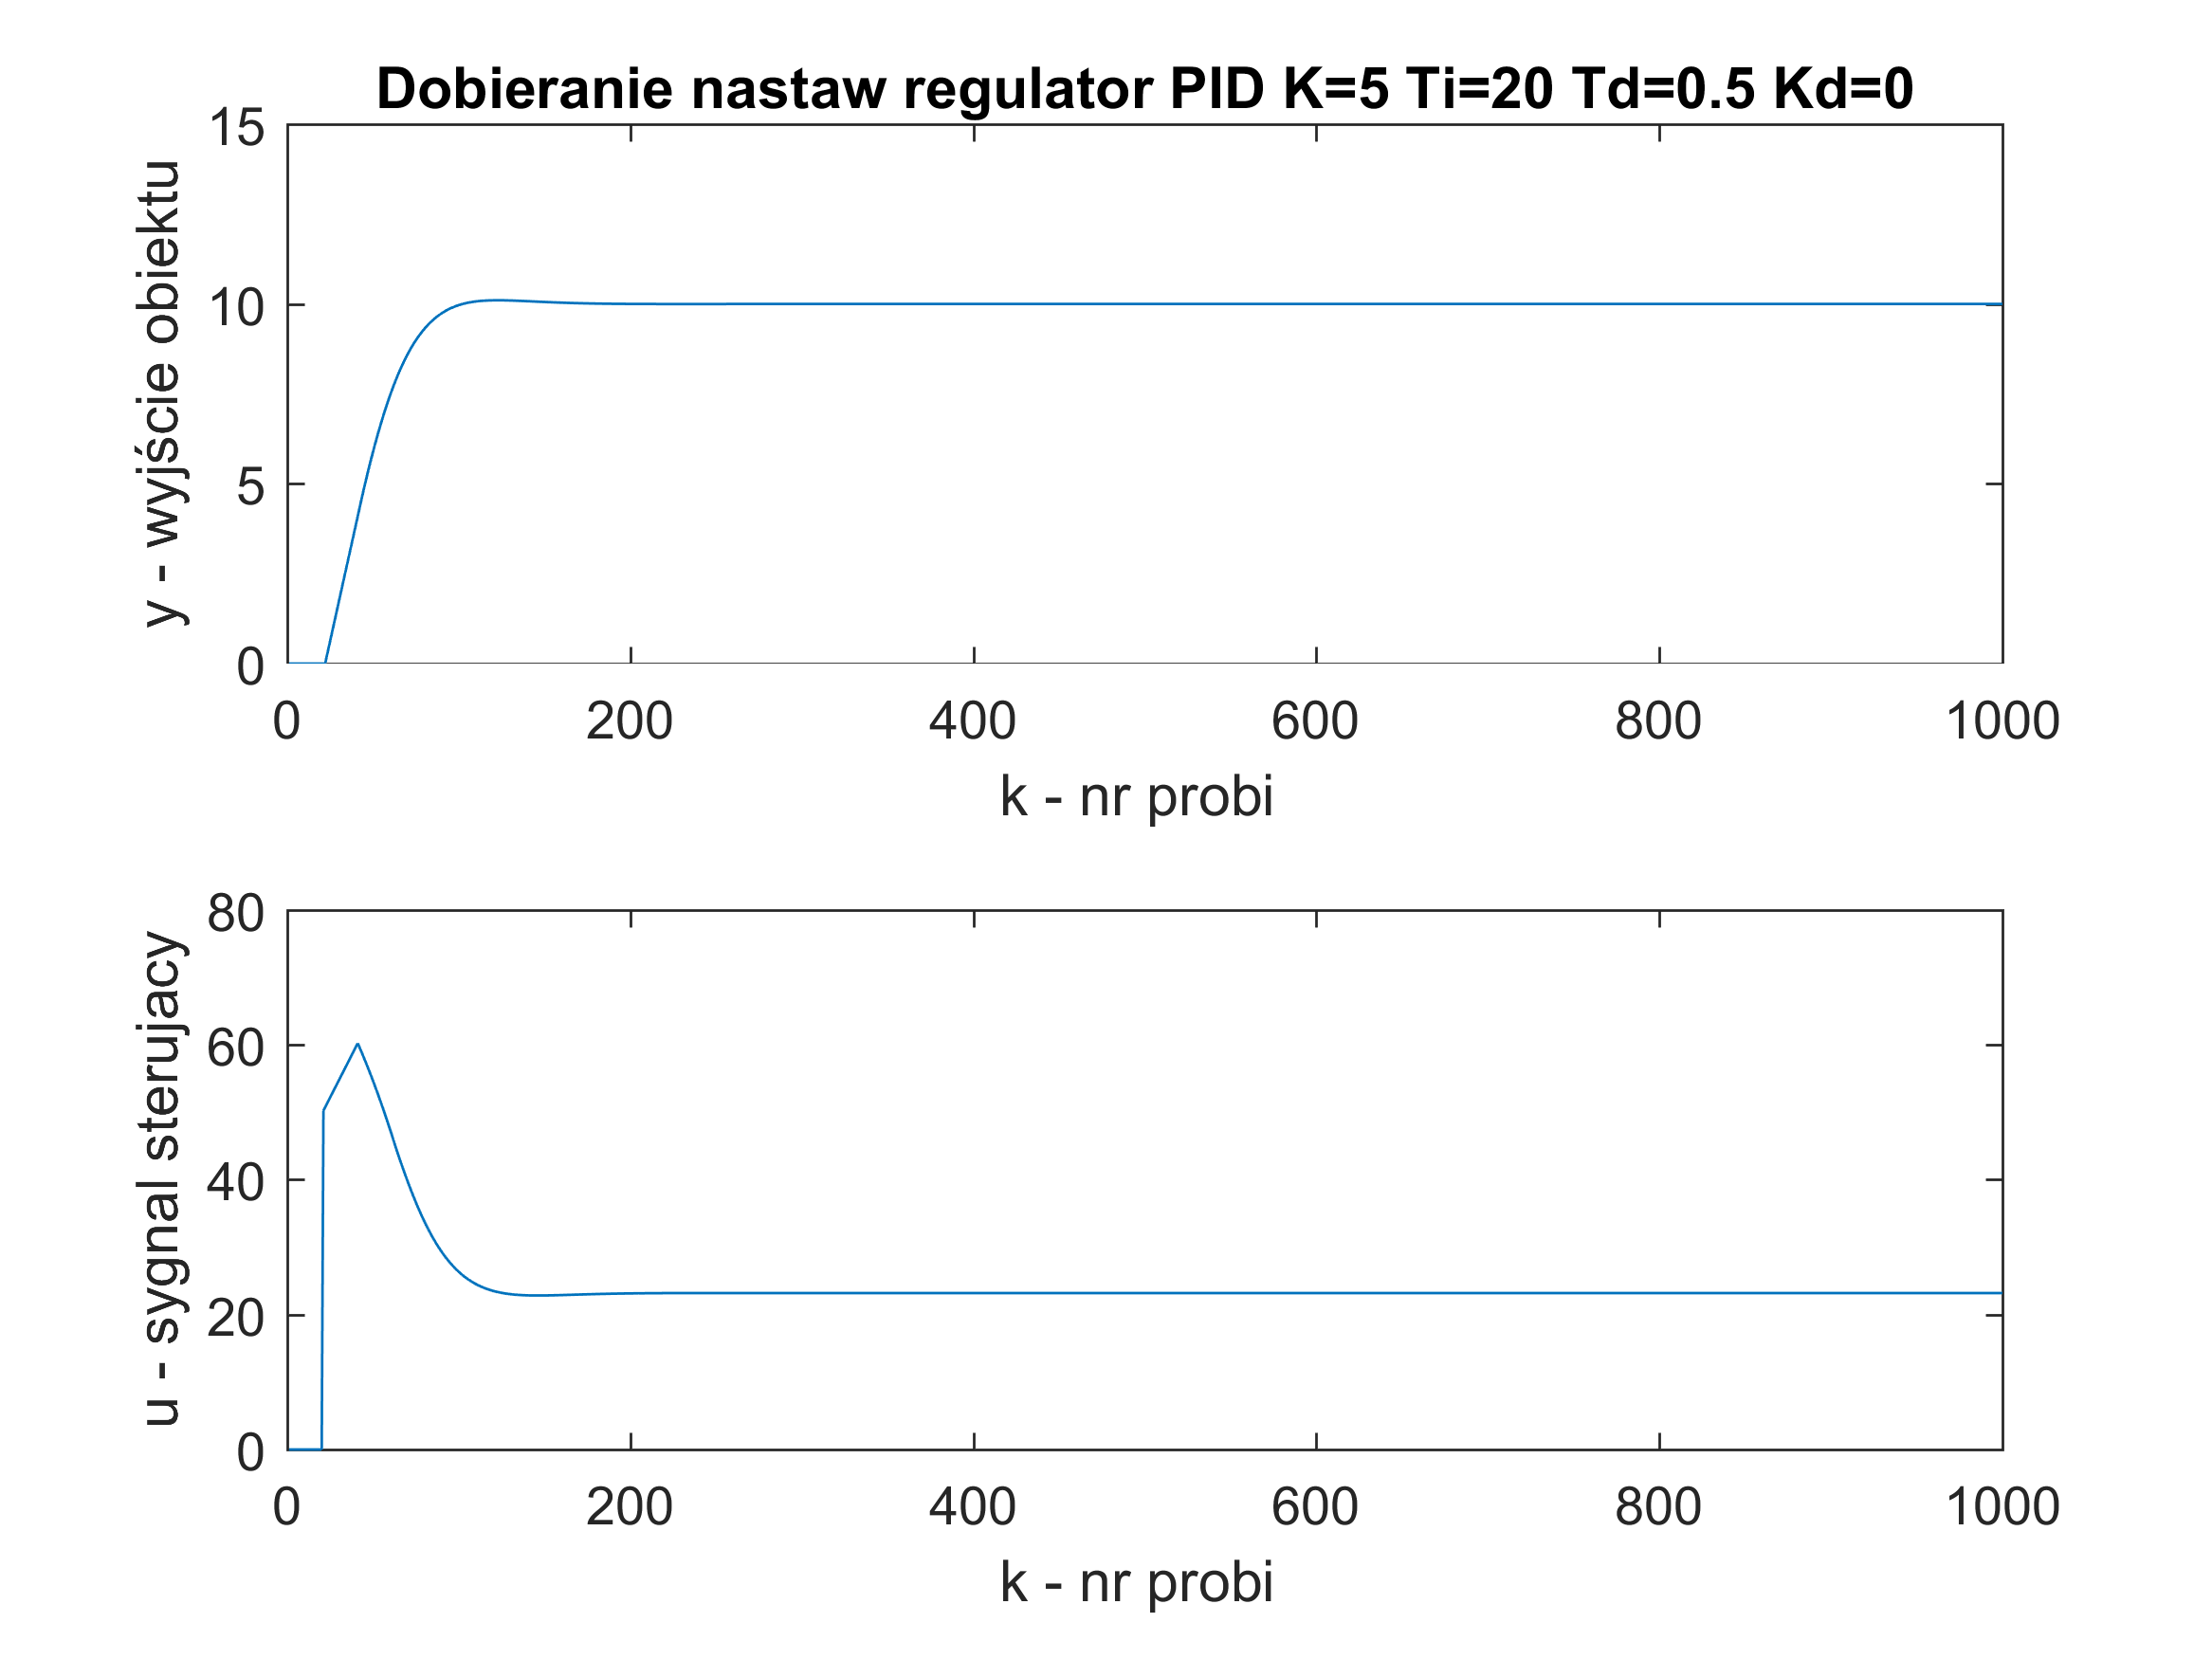
\includegraphics[width=0.9\linewidth]{pid_4.png}
	\caption{}
\end{figure}

Jak widzimy wyjście obiketu miało coraz mniejsze przeregulowanie dla rosnących wartości $T_{i}$. Przbieg sygnału sterującego zachowywał się praktycnie tak samo dla różnych $T_{i}$. Ostatecznie do naszego regulatora wybraliśmy wartość $T_{i} = 20$.

Tak wyznaczone nastawy PID zostały przez nas użyte do regulacji rzeczywistego obiektu jakim była grzałka. Dokonaliśmy jeszcze małych zmian parametrów PID, ponieważ obiekt modelowany nie oddaje w pełni zachowania obiektu w świecie rzeczywistym. Jak się okazało podczas dalszych testów na stanowisku grzejąco-chłodzącym zmiany te wpłynęły pozytywnie na prędkość osiągania zadawanego punktu pracy przez grzałkę. 

\begin{figure}[H]
	\centering
	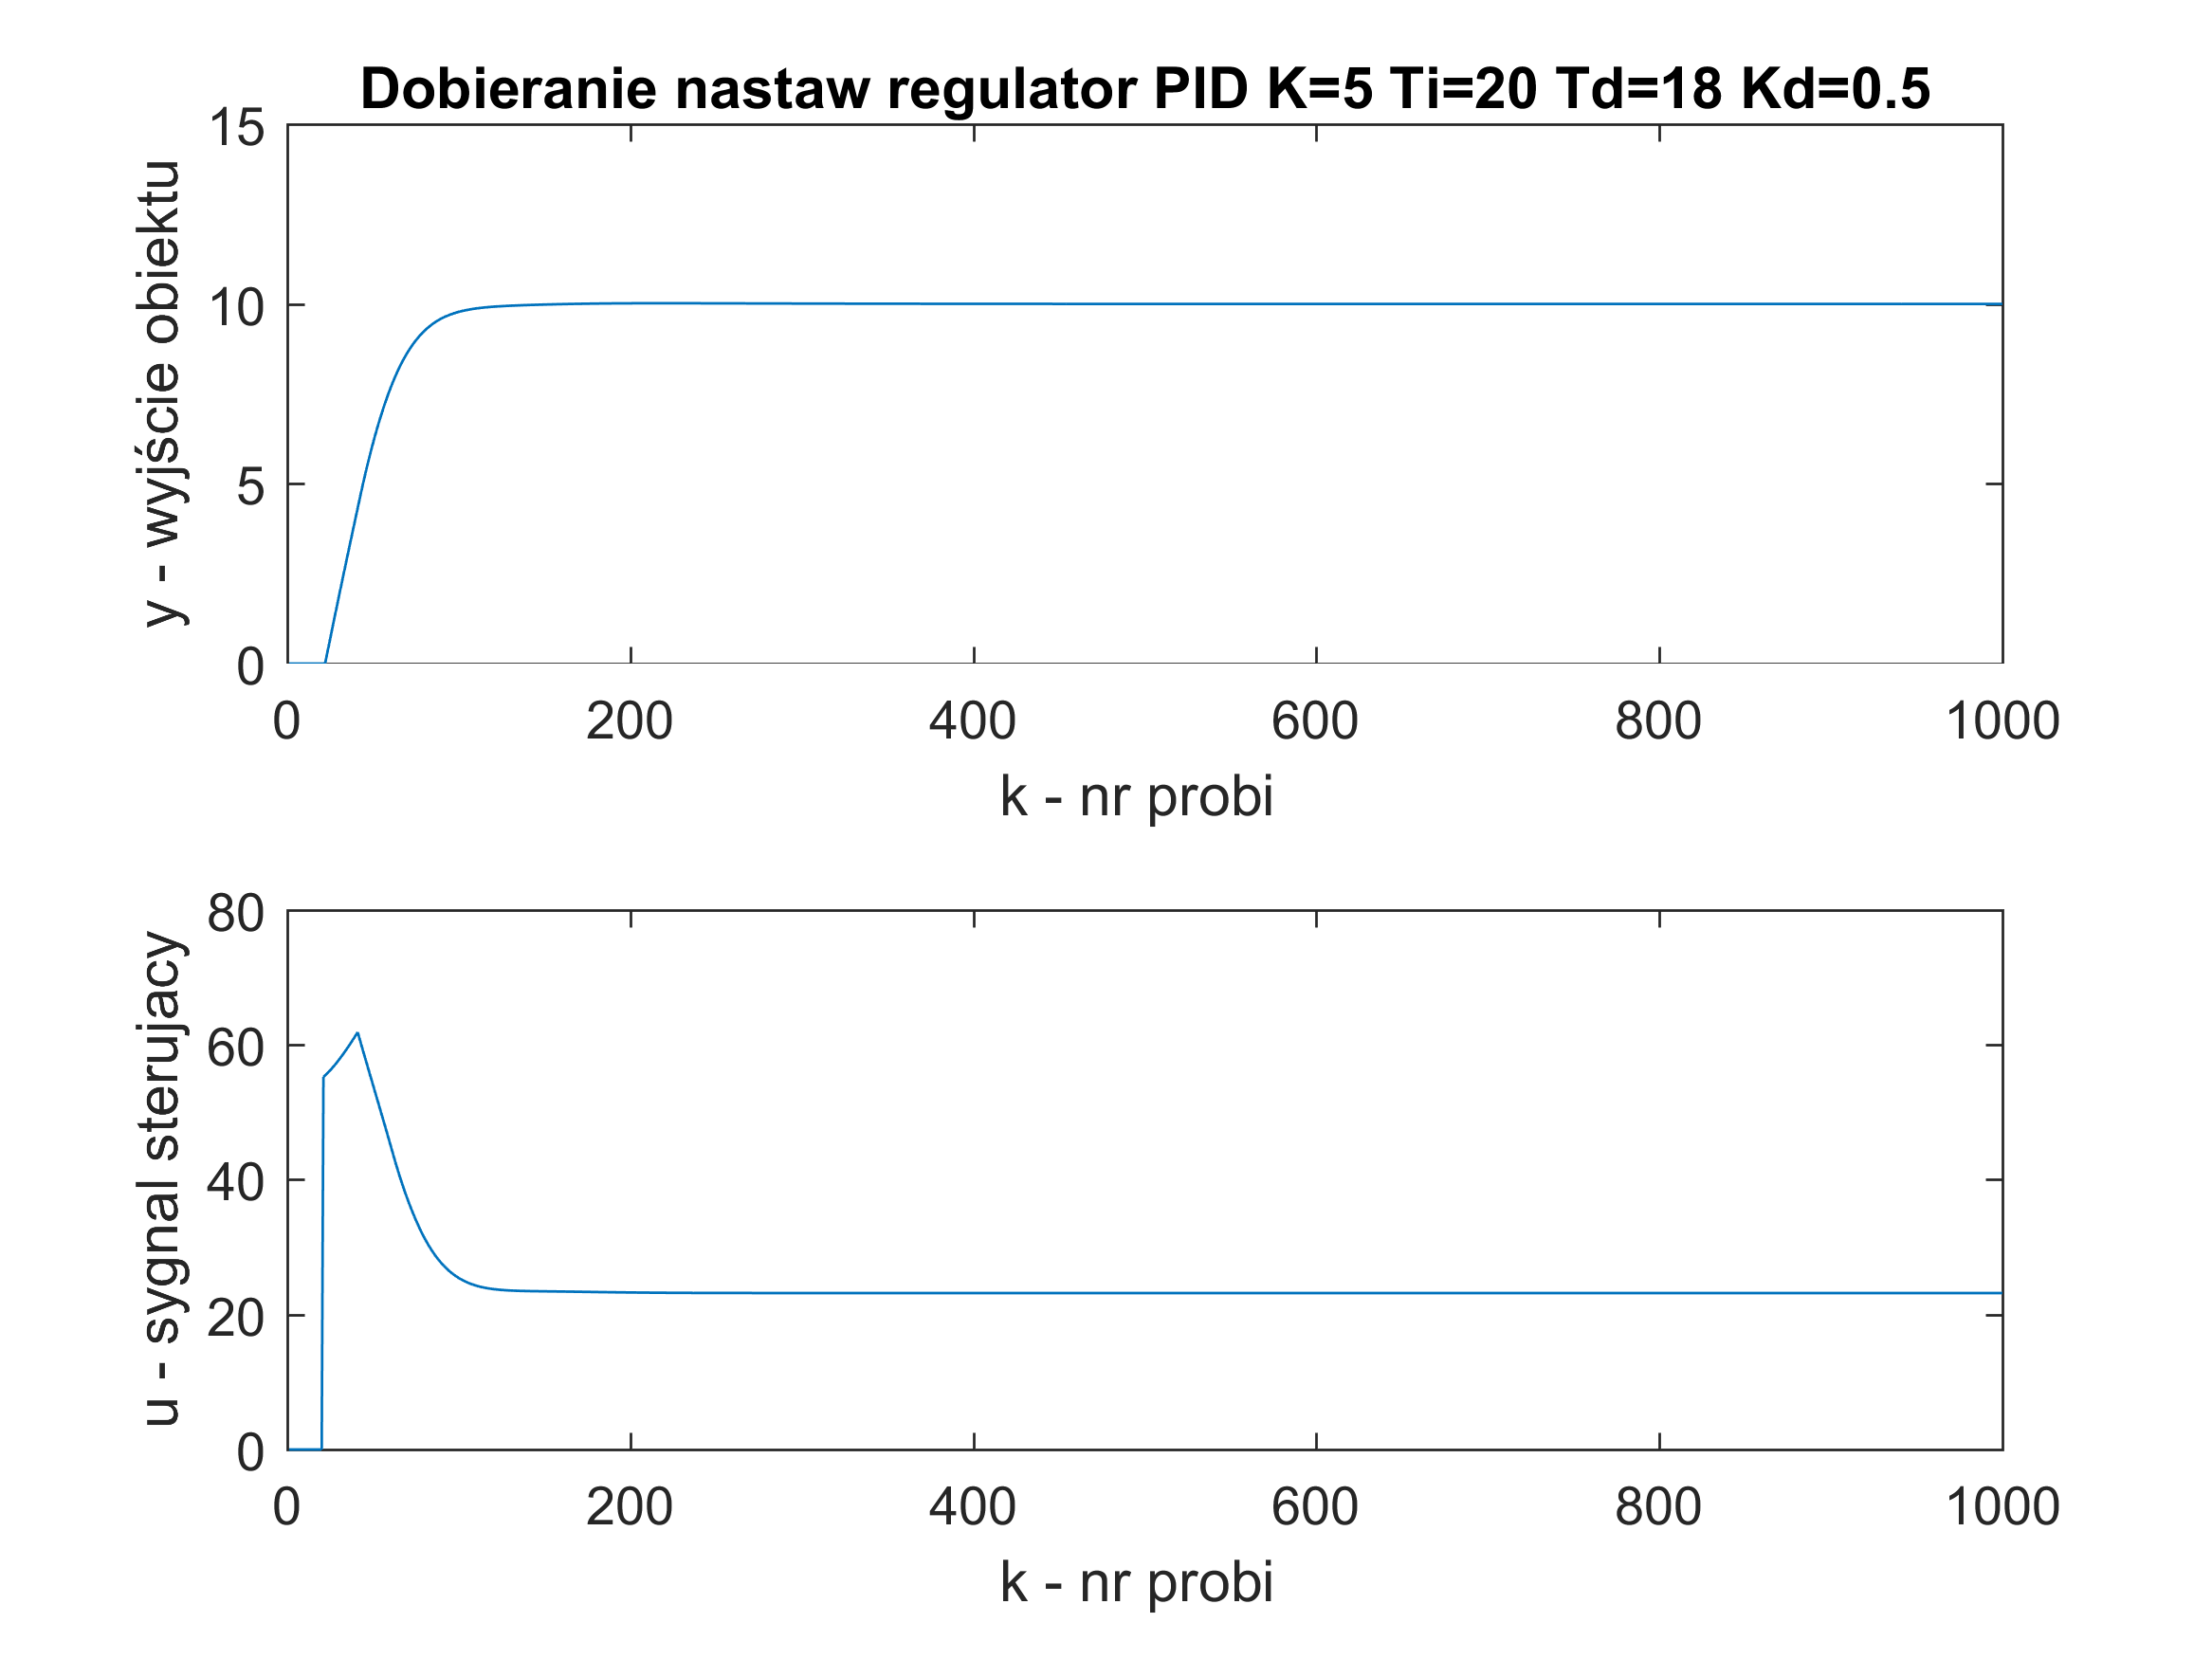
\includegraphics[width=0.9\linewidth]{pid_ostateczny.png}
	\caption{}
\end{figure}

\section{Testowanie}
Kolejnym etapem było testowanie działania stworzonej pętli regulacji poprzez sprawdzenie reakcji na zmianę temperatury zadanej oraz zmianę wartości sygnału sterującego dla wentylatora. 

\subsection{Testowanie zmiany wartości zadanej temperatury}
Najpierw wykonaliśmy testy zmiany wartości zadanej temperatury i obserwowaliśmy jak temperatura dochodzi do zadanej wartości. Wykonane zostały między innymi 4 testy: \\
1. Spadek wartości zadanej temperatury z  $40^\circ$ na $38^\circ$ (Rysunek \ref{fig:SKOK_STEROWANIA}) \\
2. Spadek wartości zadanej temperatury z  $44^\circ$ na $37^\circ$ (Rysunek \ref{fig:sterowanie4337}) \\
3. Wzrost wartości zadanej temperatury z  $38^\circ$ na $41^\circ$, przy zakłóceniu: sterowanie wentylatora = 20 (Rysunek \ref{fig:wiatrak20temp3841}) \\
4. Wzrost wartości zadanej temperatury z  $38^\circ$ na $43^\circ$, przy zakłóceniu: sterowanie wentylatora = 30  (Rysunek \ref{fig:sterowanie3843}) \\

\begin{figure}[H]
	\centering
	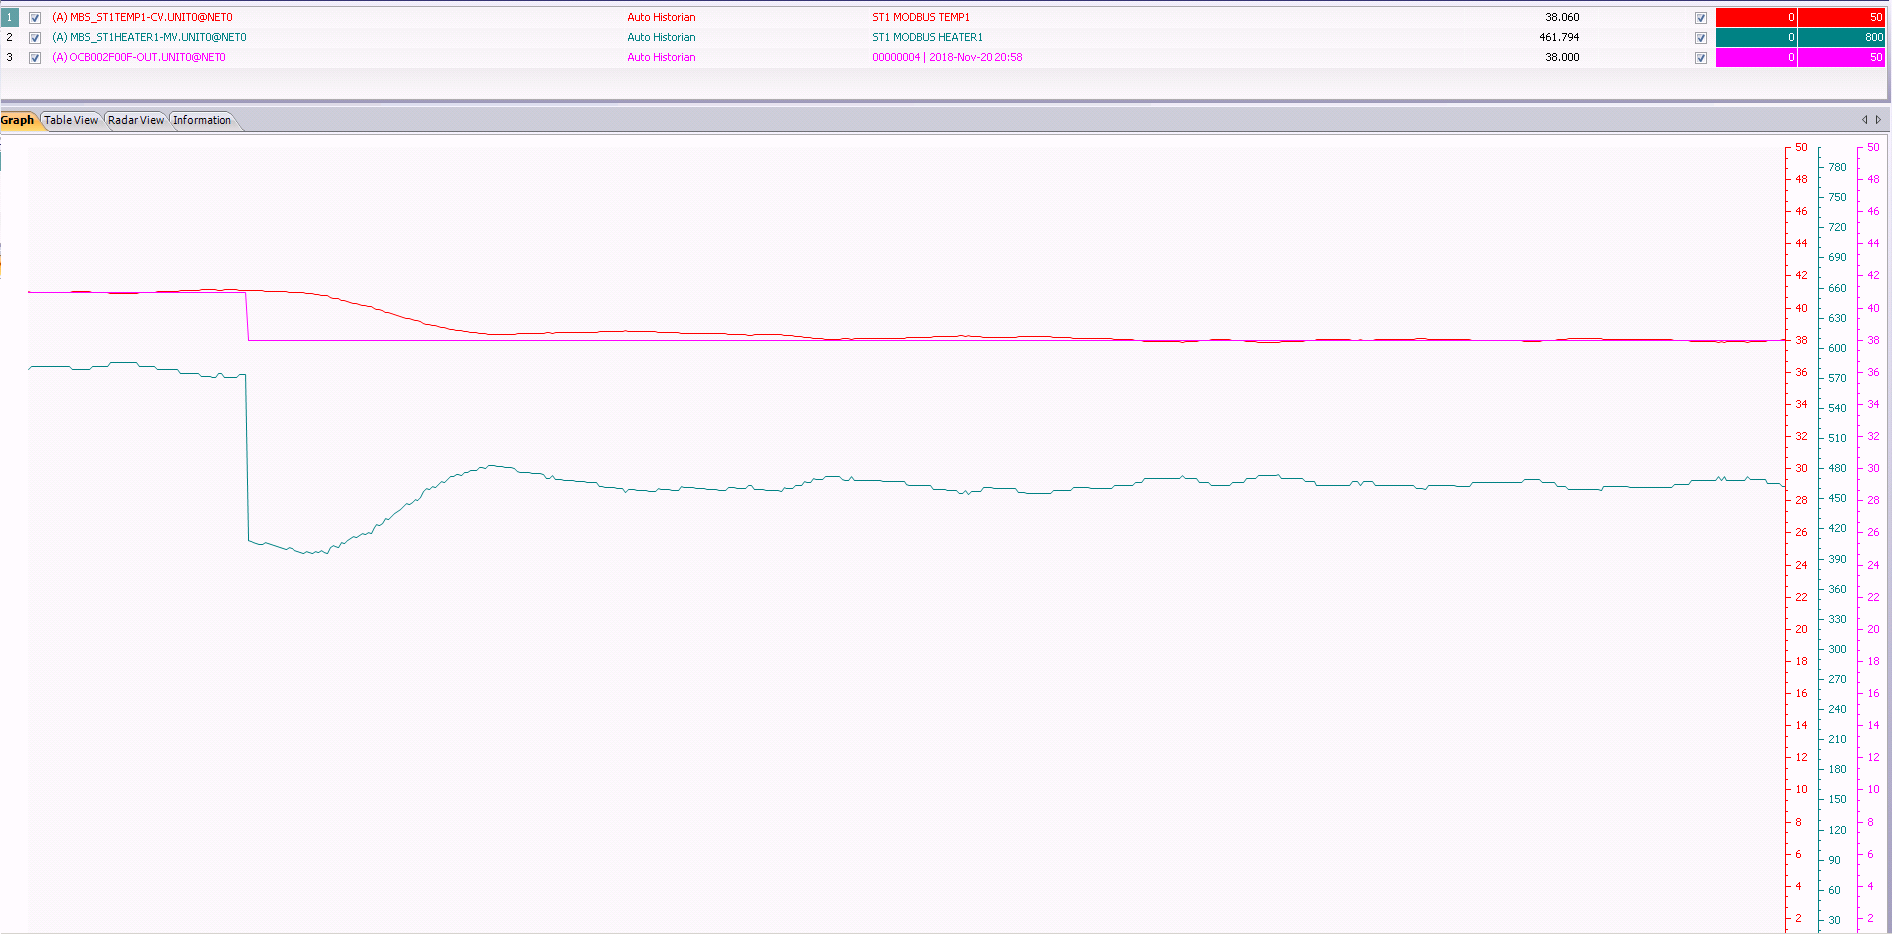
\includegraphics[width=0.9\linewidth]{SKOK_STEROWANIA}
	\caption{Zmiana wartości zadanej temperatury z  $40^\circ$ na $38^\circ$; czerwony - osiągnięta temperatura, różowy - wartość zadana temperatury, morski - sterowanie  grzałki}
	\label{fig:SKOK_STEROWANIA}
\end{figure}
\begin{figure}[H]
	\centering
	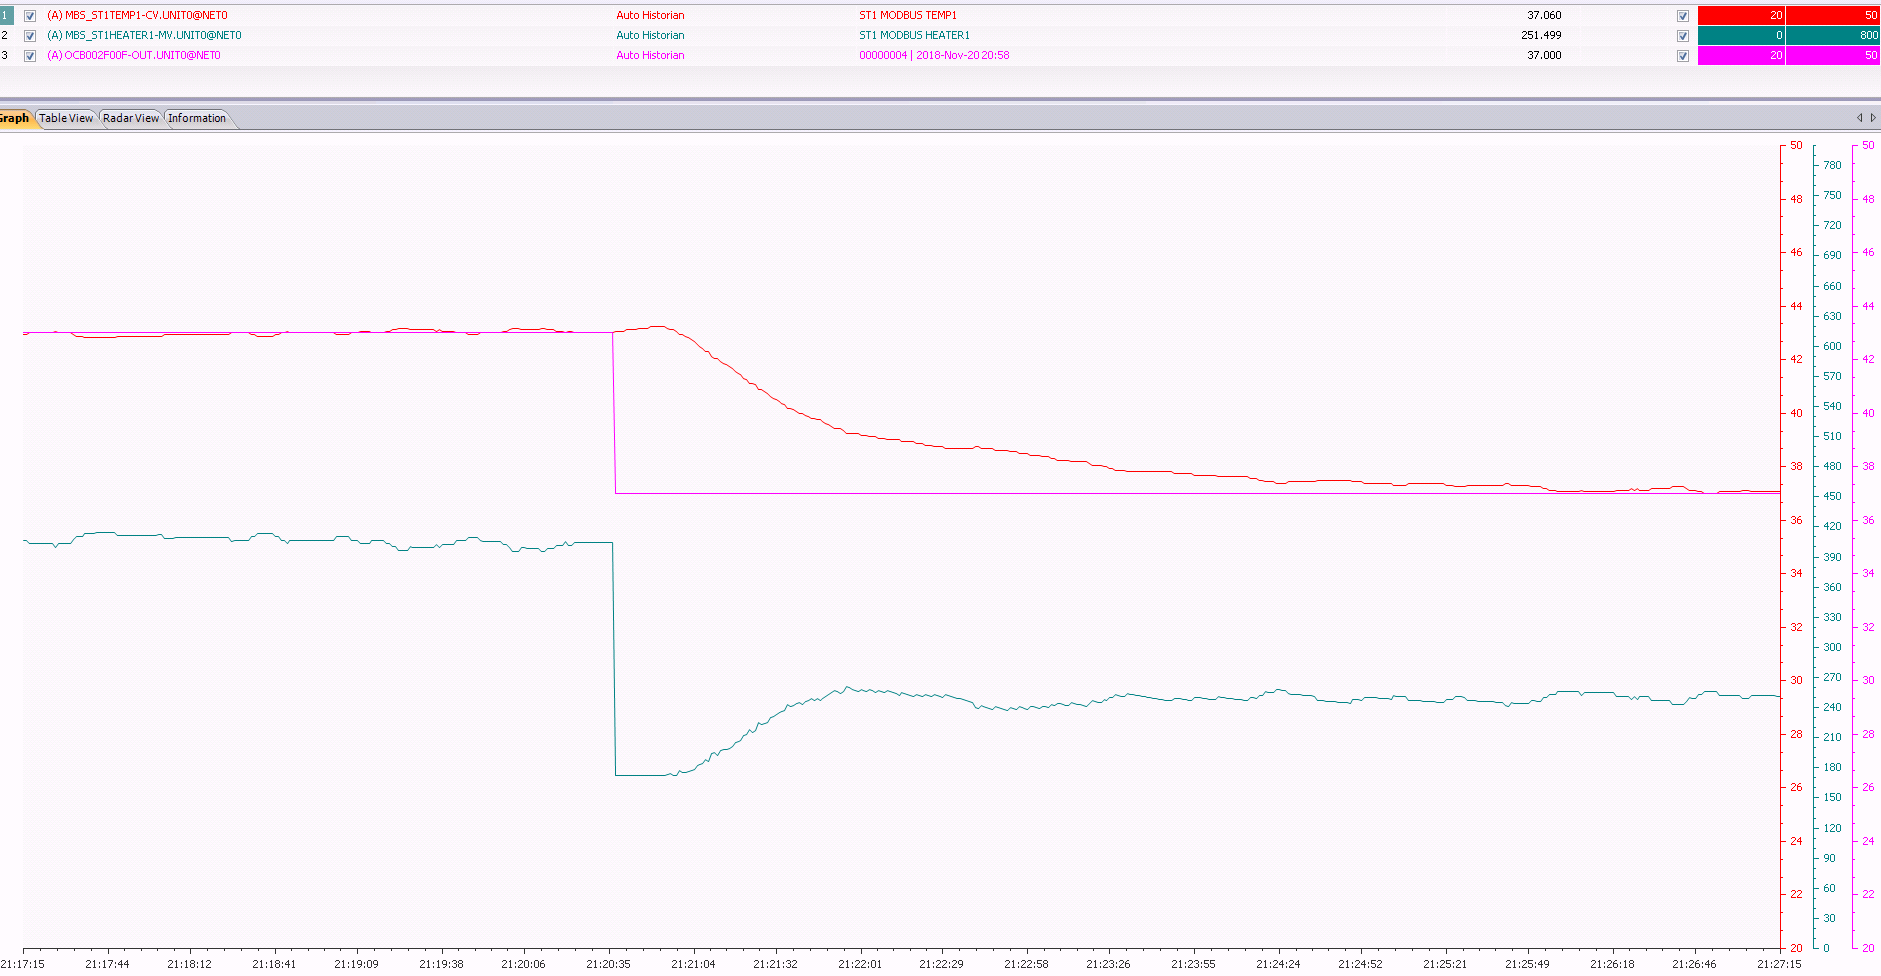
\includegraphics[width=0.9\linewidth]{sterowanie4337}
	\caption{Zmiana wartości zadanej temperatury z  $43^\circ$ na $37^\circ$; czerwony - osiągnięta temperatura, różowy - wartość zadana temperatury, morski - sterowanie  grzałki}
	\label{fig:sterowanie4337}
\end{figure}
\begin{figure}[H]
	\centering
	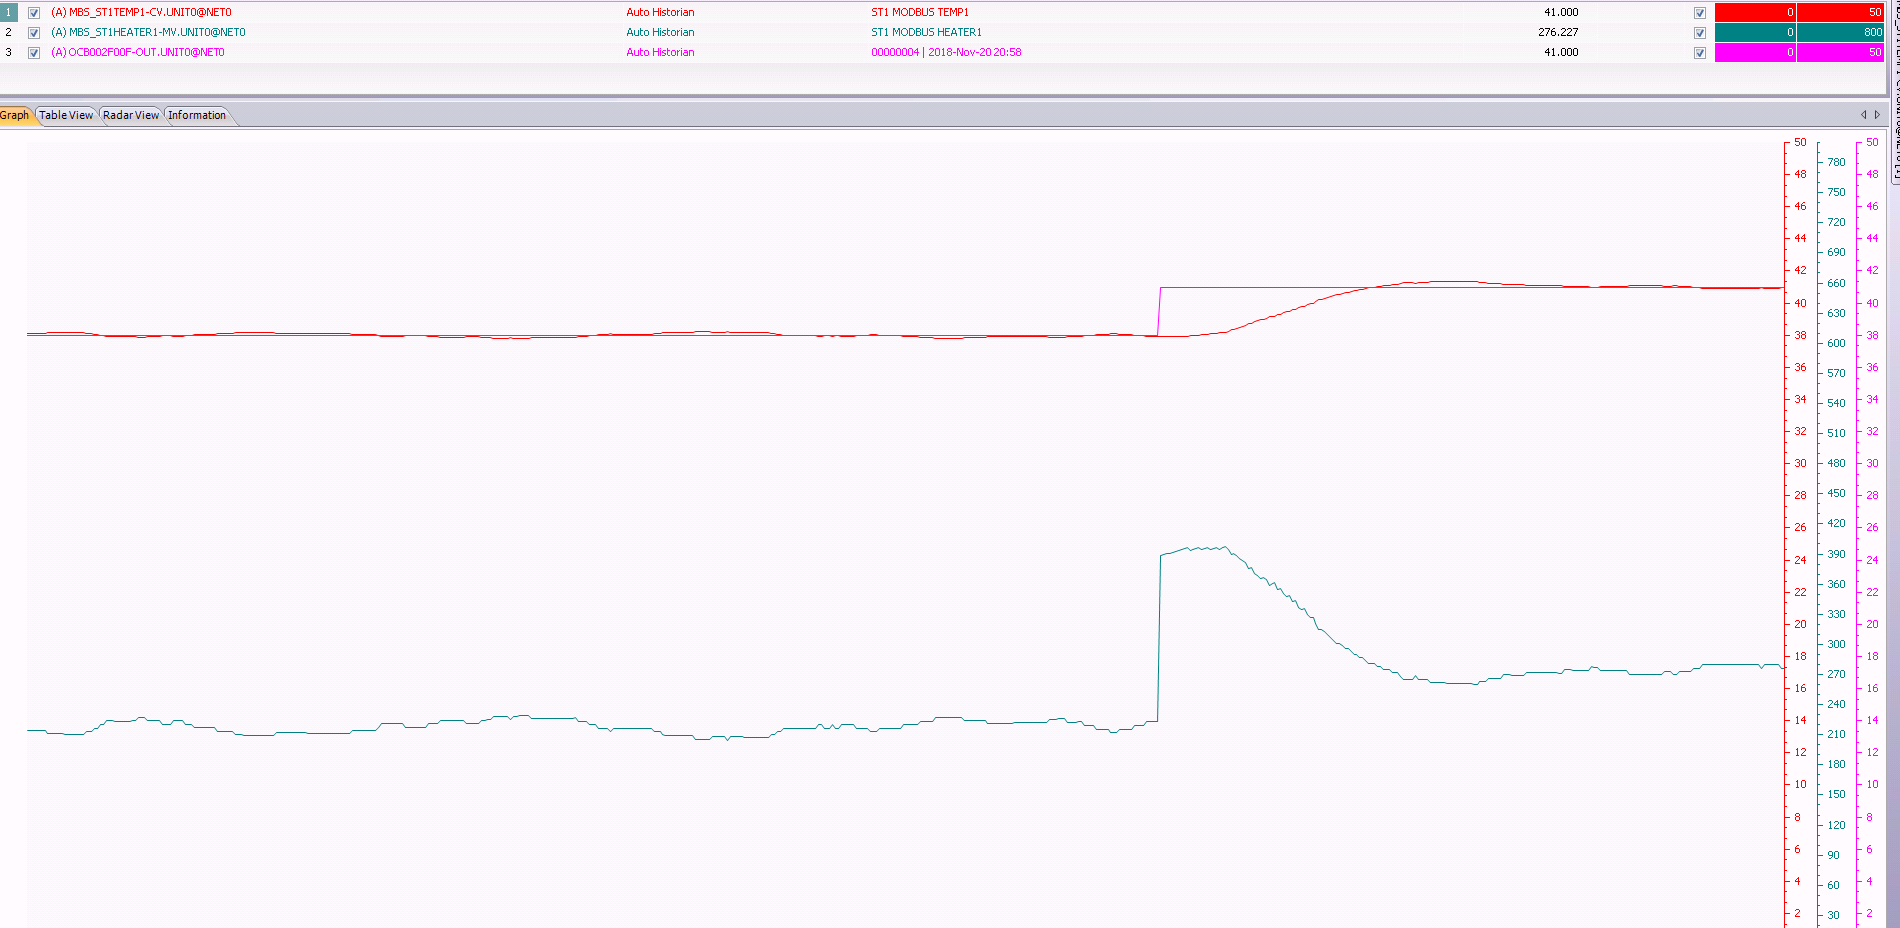
\includegraphics[width=0.9\linewidth]{wiatrak20temp3841}
	\caption{Zmiana wartości zadanej temperatury z  $38^\circ$ na $41^\circ$; czerwony - osiągnięta temperatura, różowy - wartość zadana temperatury, morski - sterowanie  grzałki}
	\label{fig:wiatrak20temp3841}
\end{figure}
\begin{figure}[H]
	\centering
	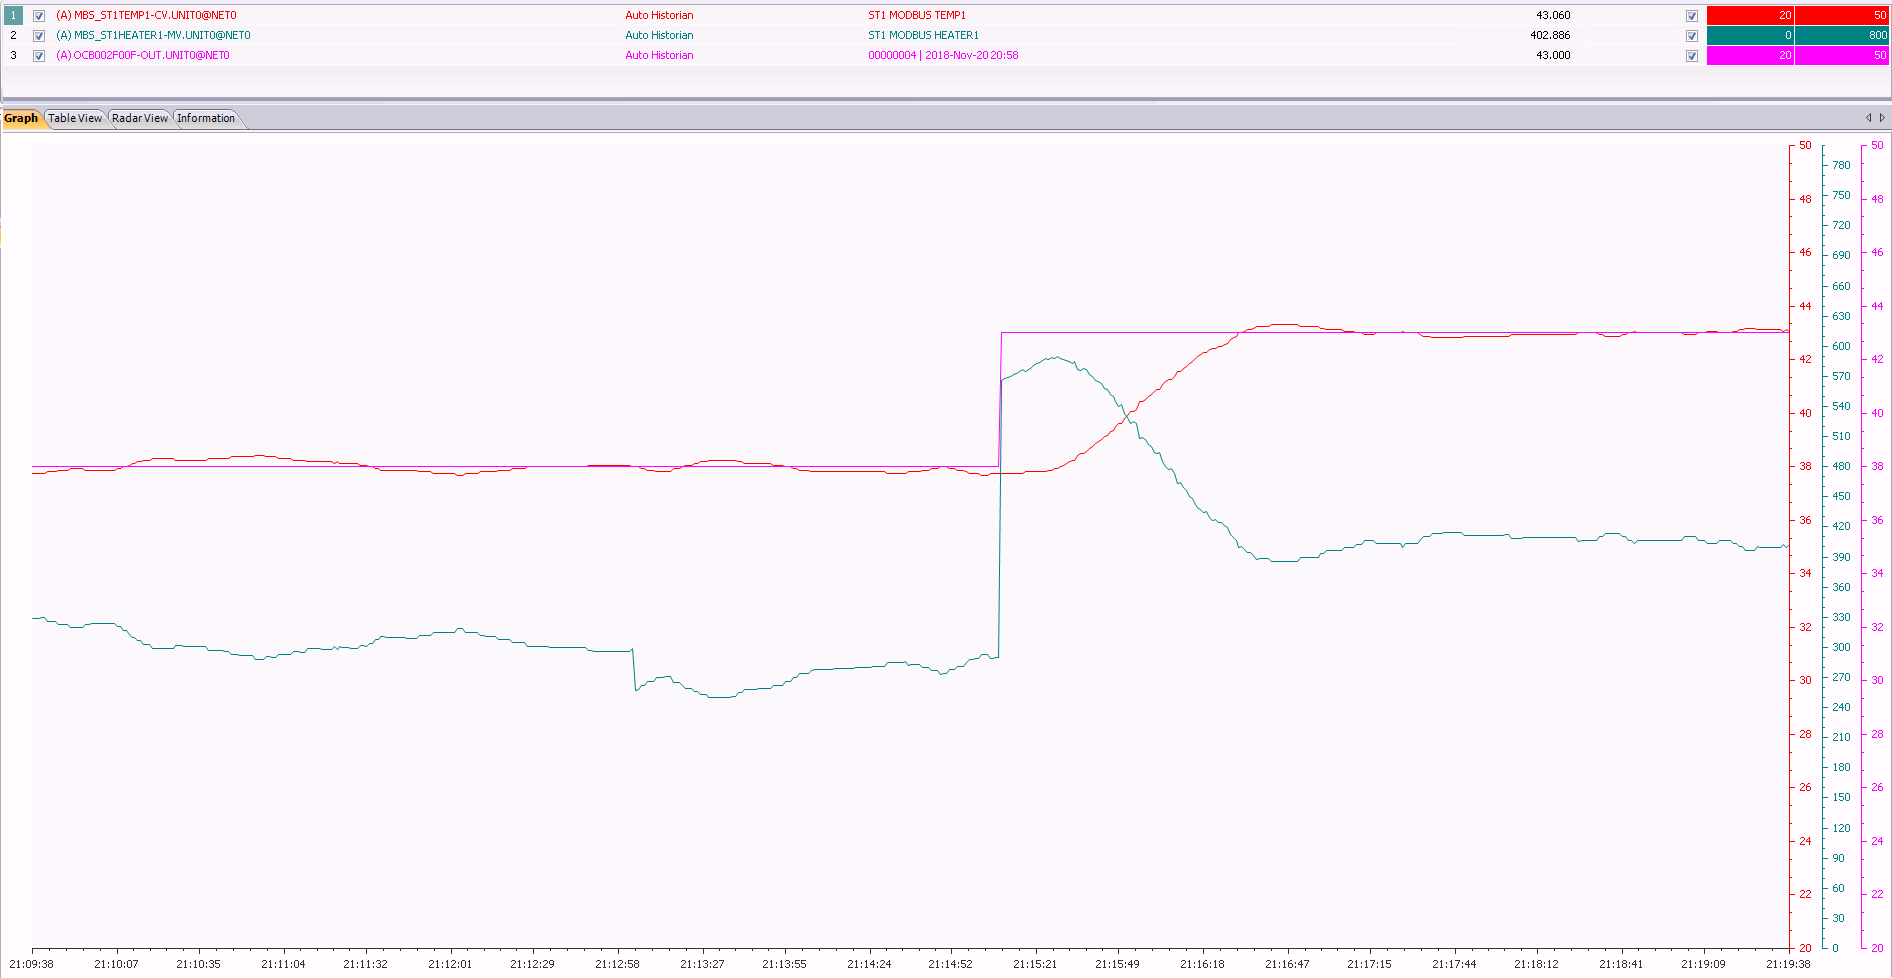
\includegraphics[width=0.9\linewidth]{sterowanie3843}
	\caption{Zmiana wartości zadanej temperatury z  $38^\circ$ na $43^\circ$; czerwony - osiągnięta temperatura, różowy - wartość zadana temperatury, morski - sterowanie  grzałki}
	\label{fig:sterowanie3843}
\end{figure}

Porównując wykresy możemy zauważyć, że obiekt szybciej osiąga zadaną temperaturę jeżeli wykonujemy skok zadanej wartości w górę do wartości zadanej (zwiększamy zadaną temperaturę) niż gdy zmniejszamy wartość zadaną (obnizamy zadaną temperaturę). Obiekt wolniej się chłodzi niż nagrzewa, co wynika z tego, że sterujemy tylko grzałką: przy zmniejszaniu temperatury czekamy aż obiekt odda ciepło do otoczenia przy obniżonym sterowaniu grzałki, podwyższając temperaturę podwyższamy po prostu wartość sterowania grzałki.  

Wynika to także z dobranego regulatora. Spadek wartości sygnału wyjściowego obiektu dla zmniejszonej wartosci zadanej temperatury na początku jest szybki (Rysunki: \ref{fig:SKOK_STEROWANIA}, \ref{fig:sterowanie4337}), ale w pobliżu wartości zadanej prędkość zniejszania się wartości temperatury znacząco spada. Dzięki temu unikamy przeregulowania i oscylacji. Podobnie jest przy wzroście sygnału wyjściowego obiektu dla zwiększonej wartosci zadanej temperatury  (Rysunki: \ref{fig:wiatrak20temp3841}, \ref{fig:sterowanie3843} przy czym tutaj można zauważyć niewielkie przeregulowanie. 

Otrzymany regulator sprawia, że wyjście obiektu dość wolno dąży do wartości zadanej, nie występują oscylacje (pomijając oscylacje wynikające z szumów pomiarowych) i występuje znikome lub niewielkie przeregulowanie. Poza tym uzyskaliśmy sygnał sterujący, który ma dość łagodny przebieg i nie za dużą amplitudę. Uzyskaliśmy także zerowy uchyb - osiągnęliśmy zadaną temperaturę. 

Warto zauważyć także różnice w wartościach sygnału sterujacego na początku przebiegów przedstawionych na rysunkach  \ref{fig:wiatrak20temp3841}, \ref{fig:sterowanie3843}. Dla pierwszego wartość sterowania zakłóceniem jest równa 30 (wentylator mocniej wieje), dla drugiego 20 (wentylator słabiej wieje). Odzwierciedla to sygnał sterujący grzałką. Dla pierwszego z podanych rysunków sygnał sterujacy ma wartość około 270, a dla drugiego 210. Jest to logiczne, ponieważ w pierwszej sytuacji grzałka musi mocniej grzeć żeby niwelować większe zakłócenie.

\subsection{Testowanie zmiany zakłócenia}
Nastepnie wykonaliśmy testy zmiany wartości zakłócenia i obserwowaliśmy jak zmiana sterowania wentylatora wpływa na przebieg temperatury i sygnału sterującego. Wykonane zostały między innymi 2 testy: \\
1. Wzrost wartości zakłócenia z 20 na 60 (Rysunek \ref{fig:zaklocenia2060}) \\
2. Spadek wartości zakłócenia z 60 na 30 (Rysunek \ref{fig:zaklocenie6030}) \\

\begin{figure}[H]
	\centering
	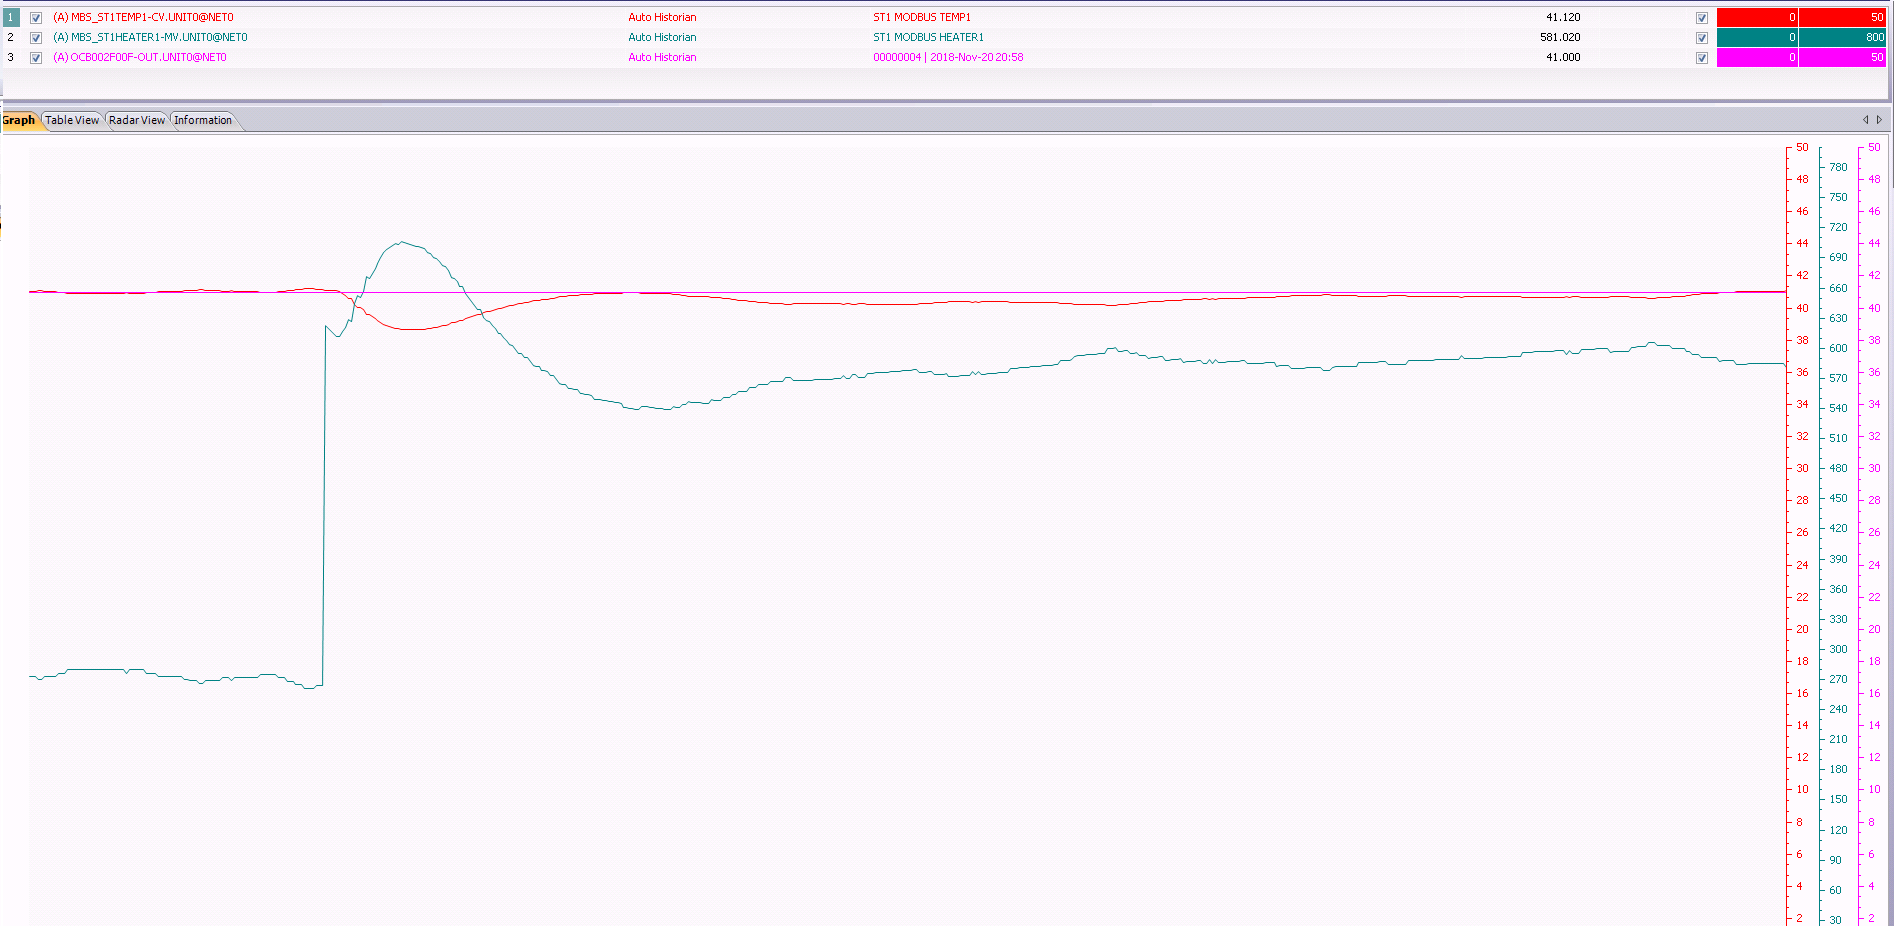
\includegraphics[width=0.9\linewidth]{zaklocenia2060}
	\caption{Wzrost wartości zakłócenia z 20 na 60; czerwony - osiągnięta temperatura, różowy - wartość zadana temperatury, morski - sterowanie  grzałki}
	\label{fig:zaklocenia2060}
\end{figure}
\begin{figure}[H]
	\centering
	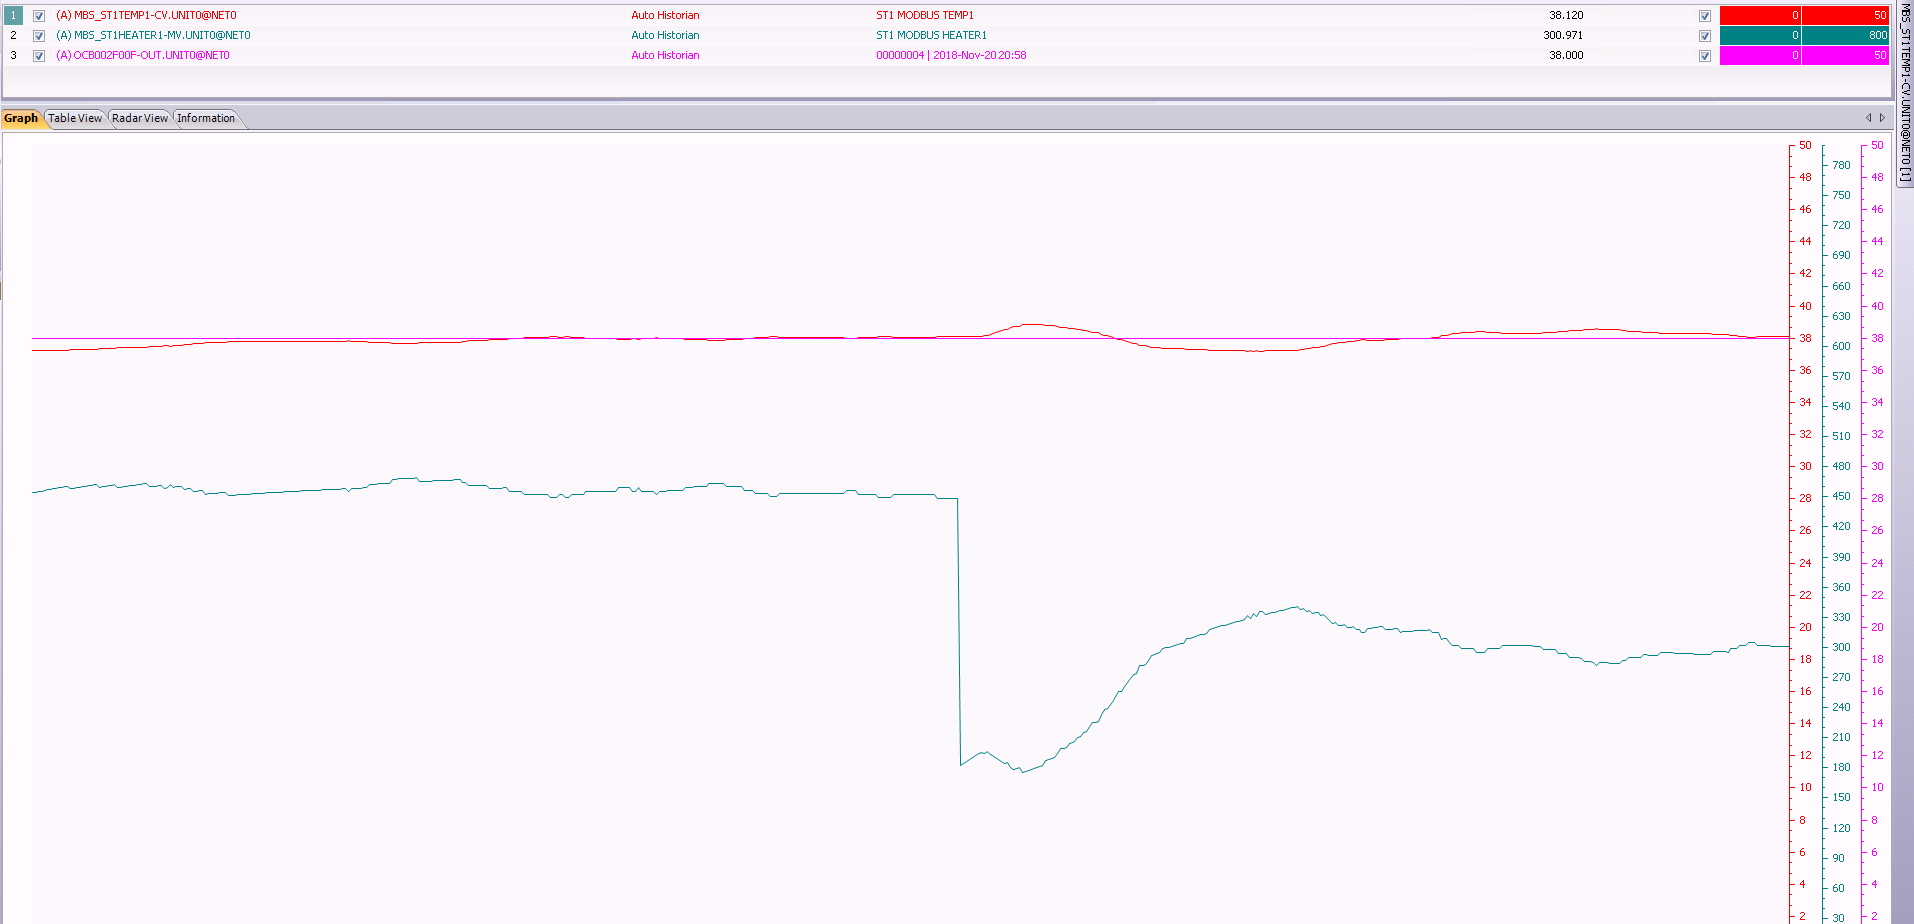
\includegraphics[width=0.9\linewidth]{zaklocenie6030}
	\caption{Spadek wartości zakłócenia z 60 na 30; czerwony - osiągnięta temperatura, różowy - wartość zadana temperatury, morski - sterowanie  grzałki}
	\label{fig:zaklocenie6030}
\end{figure}

Jako że wentylator działa szybciej niż grzałka, co widać w ich transmitancjach - wentylator ma mniejsze opóźnienie niż grzałka, nie da się całkowicie wyeliminować zakłócenia. Zanim grzałka zareaguje na zmianę zakłócenia minie wystarczajaco duża liczba próbek, aby było to widoczne na wykresie. Osiągnięta temperatura albo zwiększa się w stosunku do wartości zadanej, gdy mamy spadek na wartości sterowania wentylatora albo zmniejsza się w stosunku do wartości zadanej, gdy sterowanie wentylatora rośnie. Jest to zgodne z przewidywaniami. 

Gdy zwiękaszymy nawiew wentylatora (Rysunek \ref{fig:zaklocenia2060} - większe sterowanie), temperatura zmniejsza się. Wyliczona wartośc sterowania gwałtownie rośnie,  potem zaczyna maleć, żeby na koniec ustabilizować się na wartości większej niż początkowa (bo cały czas musi niwelować większe zakłócenie). Po czasie równym opóźnieniu grzałki, grzałka zaczyna reagować na zmianę zakłócenia i jej temperatura ponownie osiąga wartość zadaną.

Gdy zmniejszymy nawiew wentylatora (Rysunek 20 - mniejsze sterowanie), temperatura zwiększa się. Wyliczona wartośc sterowania gwałtownie maleje, potem zaczyna rosnąć, żeby na koniec ustabilizować się na wartości mniejszej niż początkowa (bo cały czas musi niwelować mniejsze zakłócenie niż na początku). Warto zwrócić uwagę, że nie da się zmniejszyć sterowania do wartości mniejszej niż 0. Po czasie równym opóźnieniu grzałki, grzałka zaczyna reagować na zmianę zakłócenia i ponownie osiągamy zadaną wartość temperatury.

Z powodu nieliniowości wentylatora (innego zachowywania się przy skoku w dół, a innego przy skoku w górę), podjęliśmy decyzję faworyzującą zmianę zakłócenia w górę. Transmitancja przy odprzęganiu jest bliższa transmitancji wentylatora wyliczonej przy wzroście zakłócenia. Z tego powodu lepiej działa odprzęganie zakłócenia, gdy wartość sterowania wentylatorem rośnie. Można to zauważyć na rysunkach, ponieważ gdy wartość sterowania wentylatorem spada, temperatura przy stabilizowaniu się na początku lekko oscyluje. Gdy wartość sterowania wentylatorem rośnie - szybciej dochodzimy do wartości zadanej i nie występują oscylacje. Dobrana transmitancja odprzęgajaca jest wystarczająca do niwelowania nie za dużych zakłóceń z wentylatora.


\subsection{Konkurs}
Ostatecznym sprawdzianem był udział w konkursie. Przebieg sygnałów uzyskanych podczas konkursu został ukazany na Rysunku \ref{fig:konkurs}. Podczas konkursu został wykonany skok wartości zadanej z $38^\circ$ na $44^\circ$. Po dojściu temperatury do zadanej wartości, zostało zmienione zakłócenie z 30 na 45. 

\begin{figure}[H]
	\centering
	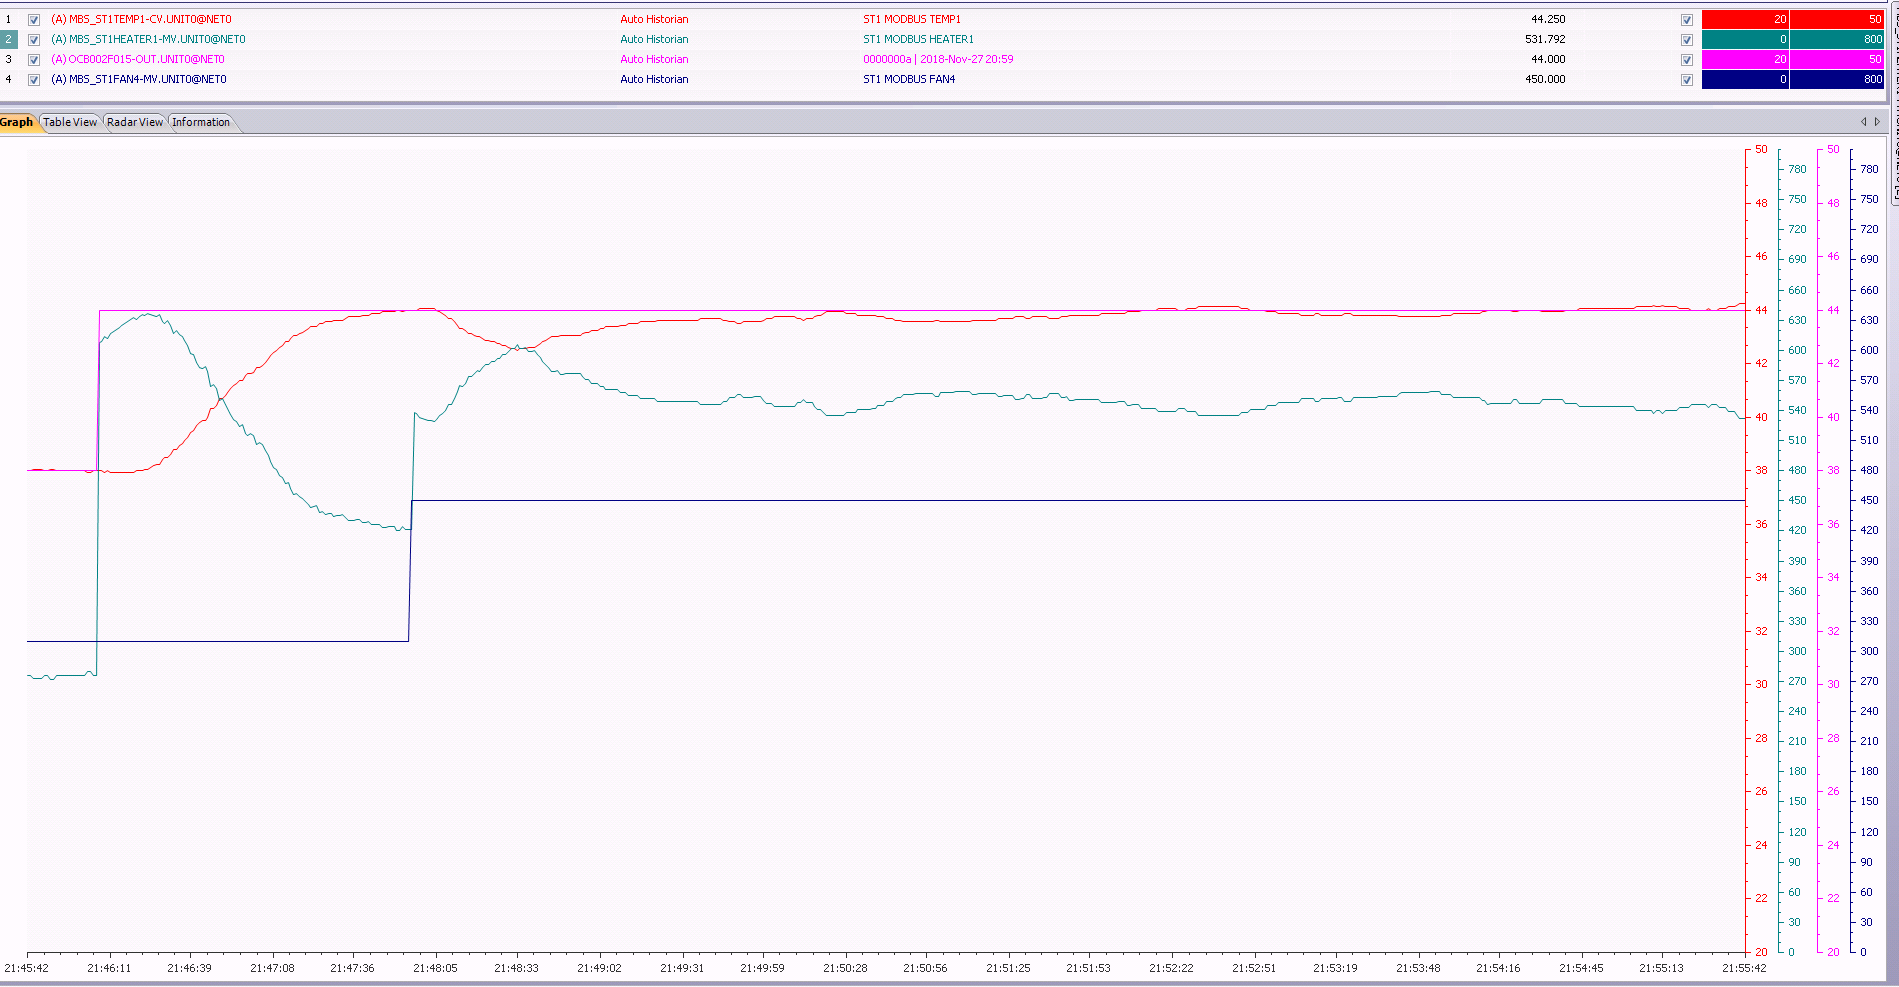
\includegraphics[width=0.9\linewidth]{konkurs}
	\caption{Wykres przebiegu sygnałów uzyskany podczas konkursu: czerwony - osiągnięta temperatura, różowy - wartość zadana temperatury, granatowy - sterowanie wentylator, morski - sterowanie  grzałki}
	\label{fig:konkurs}
\end{figure}

Przy zmianie wartości zadanej sygnał sterujący gwałtownie wzrósł, a potem zaczął maleć. Temperatura osiągnęła zadaną wartość po dwóch minutach. Zanim układ zdążył się ustabilizował zostało zmienione zakłócenie - wentylator zaczęł intensywniej pracować. Z tego powodu zmniejszyła się temperatura (nie da się całkowicie wyeliminować zakłócenia). Sygnał sterujący grzałką zwiększył swoją wartość, aby zniwelować zakłócenie. Następnie zaczął maleć, aby w końcu ustabilizować się na wartości większej niż przed skokiem zakłócenia - co jest logiczne z uwagi na to, że cały czas musi niwelować zwiększone sterowanie wentylatora. Temperatura osiagnęła spowrotem wartość zadaną

Jakość regulacji była oceniana jako suma błędów średniokwadratowych dla osiągniętej temperatury w porównaniu do wartości zadanej. Układ poradził sobie z zadanymi zmianami, czego dowodem było osiągnięcie drugiego miejsca w konkursie. 

\section{Wnioski}

Celem laboratorium było zaimplementowanie regulatora dla obiektu rzeczywistego. Wynikały z tego pewne trudności. \\
Podczas opracowywania rozwiązania dużo czasu należało poświęcić na strojenie regulatora. Obiekt terminczny charakteryzował się tym, że potrzebował dużo czasu na ustabilizowanie się. Z tego powodu wykonanie jednego eksperymentu (zarówno zebranie pojedynczej odpowiedzi skokowej, jak i eksperymenty dokonywane w celu testowania i dostrajania regulatora) zajmowało stosunkowo dużo czasu. \\
Kluczową sprawą było startowanie eksperymentów ze stanu ustalonego (szczególnie przy zbieraniu odpowiedzi skokowej) oraz odpowiednio długie oczekiwanie na ustabiliowanie się wyjścia.\\
Uzyskana odpowiedź skokowa umożliwiła nam testowanie regulatora w \textit{Matlabie}. Dzięki symulacjom w szybki sposób mogliśmy dobrać początkowe nastawy regulatora PID co znacznie usprawniło nam dostrajanie regulatora już pracując na stanowisku grzewczo-chłodzącym.\\
W zadanym obiekcie nie było możliwe całkowite odprzęganie zakłóceń. Wynika to z tego, że sygnał sterowania grzałką ma większe opóniżnienie niż, niż zakłócenia. Temperatura wolniej reagowała na zmiany sterowania grzałką, niż na zmianę  prędkości wentylatora. Oprócz tego wentylator nieliniowo wpływał na obiekt - lepsze rezultaty możnaby było uzyskać korzystając na przykład z modeli rozmytych, co z powodu ograniczonego czasu na wykonanie zadania nie zostało zaimplementowane.\\







\end{document}

